\documentclass{article}
\usepackage{geometry}
\geometry{
    top=2.5cm,
    bottom=2.5cm,
    left=2.5cm,
    right=2.5cm
}
\usepackage{float}
\usepackage{ctex}
\usepackage{longtable}
\usepackage{multirow}
\usepackage{graphicx}
\usepackage{subfigure}
\usepackage[export]{adjustbox}
\usepackage{xcolor,colortbl,xparse}
\usepackage{listings,listings-rust}
\usepackage{enumitem}
\usepackage{textcomp}
\usepackage[bottom]{footmisc}
\usepackage[T1]{fontenc}
\usepackage[hidelinks]{hyperref}
\usepackage{amssymb}
\usepackage{pifont}
\usepackage{array}
\usepackage{longtable}
\usepackage{booktabs}
\usepackage[australian]{babel}
\usepackage{datetime}
\usepackage{titlesec}

% modify list style
\renewcommand{\labelitemii}{$\circ$}

% section define
\renewcommand\thesection{\chinese{section}、} % don't modify
\renewcommand\thesubsection{\arabic{section}\thinspace.\thinspace\arabic{subsection}}
\renewcommand\thesubsubsection{\thesubsection\thinspace.\thinspace\arabic{subsubsection}}

% font & font size
\newcommand{\sihao}{\fontsize{14pt}{3.2pt}\selectfont}
\newcommand*{\AdobeHT}{\CJKfamily{AHT}}
\newcommand{\xiaosihao}{\fontsize{12.1pt}{\baselineskip}\selectfont}
\newcommand{\xiaosanhao}{\fontsize{15.1pt}{2pt}\selectfont}
\newcommand{\sanhao}{\fontsize{15.75}{\baselineskip}\selectfont}

% section and title definiation
\titleformat{\section}{\sanhao\heiti\centering}{\thesection}{0em}{}
\titleformat{\subsection}{\sihao\heiti}{\thesubsection}{1em}{}
\titleformat{\subsubsection}{\xiaosihao\heiti}{\thesubsubsection}{1em}{}

% default line space config
\newcommand{\defaultlinespread}{1.35}
\linespread{\defaultlinespread}

% english fonts
\usepackage{fontspec}
\setmainfont{Times New Roman}
% \setsansfont{Arial}
% \setmonofont{Courier New}

% title & author
\newcommand{\titlestr}{NoAxiom OS}
\newcommand{\authorstr}{陈润澎,刘文涛}

\begin{document}

% title
\begin{titlepage}
\centering

\includegraphics[width=0.5\textwidth]{assets/title/hdu.png}

\vspace{3cm}

\includegraphics[width=0.3\textwidth]{assets/title/NoAxiom.png}

\vspace{.5cm}
{\LARGE \bf{\titlestr} \par}

\vspace{.1cm}
{\Large {\it{Operating System Design Manual} } \par}

\vspace{7cm}
{\Large \authorstr \par}
\vspace{.1cm}
\today
\vfill
\end{titlepage}

% contents
\tableofcontents

% color define
\definecolor{Gray}{gray}{0.85}
\definecolor{codegreen}{rgb}{0,0.6,0}
\definecolor{codegray}{rgb}{0.5,0.5,0.5}
\definecolor{codepurple}{rgb}{0.58,0,0.82}
\definecolor{bkgray}{HTML}{f8f9fa}
\definecolor{edgegray}{HTML}{e8eaed}
\definecolor{codepurple}{rgb}{0.58,0,0.82}
\definecolor{bkgray}{rgb}{0.95,0.95,0.95}
\definecolor{edgegray}{rgb}{0.8,0.8,0.8}
\definecolor{codeblue}{rgb}{0.2,0.2,0.8}
\definecolor{keywordorange}{rgb}{0.8,0.4,0}
\definecolor{keywordred}{rgb}{0.8,0,0}
\definecolor{keywordcyan}{rgb}{0,0.6,0.6}

% rust syntax define
\newpage
\lstset{
    language=Rust,
    breaklines=true,
    numbers = left,
    numberstyle=\smallskip,
    commentstyle=\color{codegreen},
    keywordstyle=\color{blue},
    keywordstyle=[1]\color{codepurple},
    keywordstyle=[2]\color{blue},
    keywordstyle=[3]\color{blue},
    numberstyle=\tiny\color{codegray},
    stringstyle=\color{codepurple},  
    basicstyle=\ttfamily\small,
    lineskip=1pt,
    backgroundcolor = \color{bkgray},
    showstringspaces=false,
    frame=single,
    frameround=tttt,
    rulecolor=\color{edgegray},
    upquote=true,
}
\newcommand{\code}[1]{\colorbox{bkgray}{\lstinline|#1|}}

% redefine figure and table's prefix
\renewcommand{\figurename}{图}
\renewcommand{\tablename}{表}
\renewcommand{\figureautorefname}{图}
\renewcommand{\tableautorefname}{表}
\renewcommand{\arraystretch}{0.9}

\newpage
\section{概述}
\subsection{系统简介}

NoAxiom操作系统\footnote{https://github.com/NoAxiom/NoAxiom-OS}是一款由杭州电子科技大学NoAxiom团队\footnote{https://github.com/NoAxiom}开发的基于Rust语言的宏内核操作系统,可同时于RISC-V64平台和LoongArch64平台运行。本操作系统自主实现了\textbf{进程管理、内存管理、文件系统、任务调度、信号系统、时钟模块、网络模块、硬件抽象层}等子模块,并基于Rust无栈协程异步语法实现\textbf{异步调度},在IO等方面取得了优异的性能水平。

\subsection{系统整体架构}

NoAxiom操作系统可分为四个层次:\textbf{机器层、硬件抽象层、内核实现层、用户层},此外还有全局设置子模块用于在各个层级之间传递设置信息与常量定义信息。\autoref{fig:noaxiom_structure}中展示了NoAxiom的整体架构设计图。

\begin{figure}[H]
    \centering
    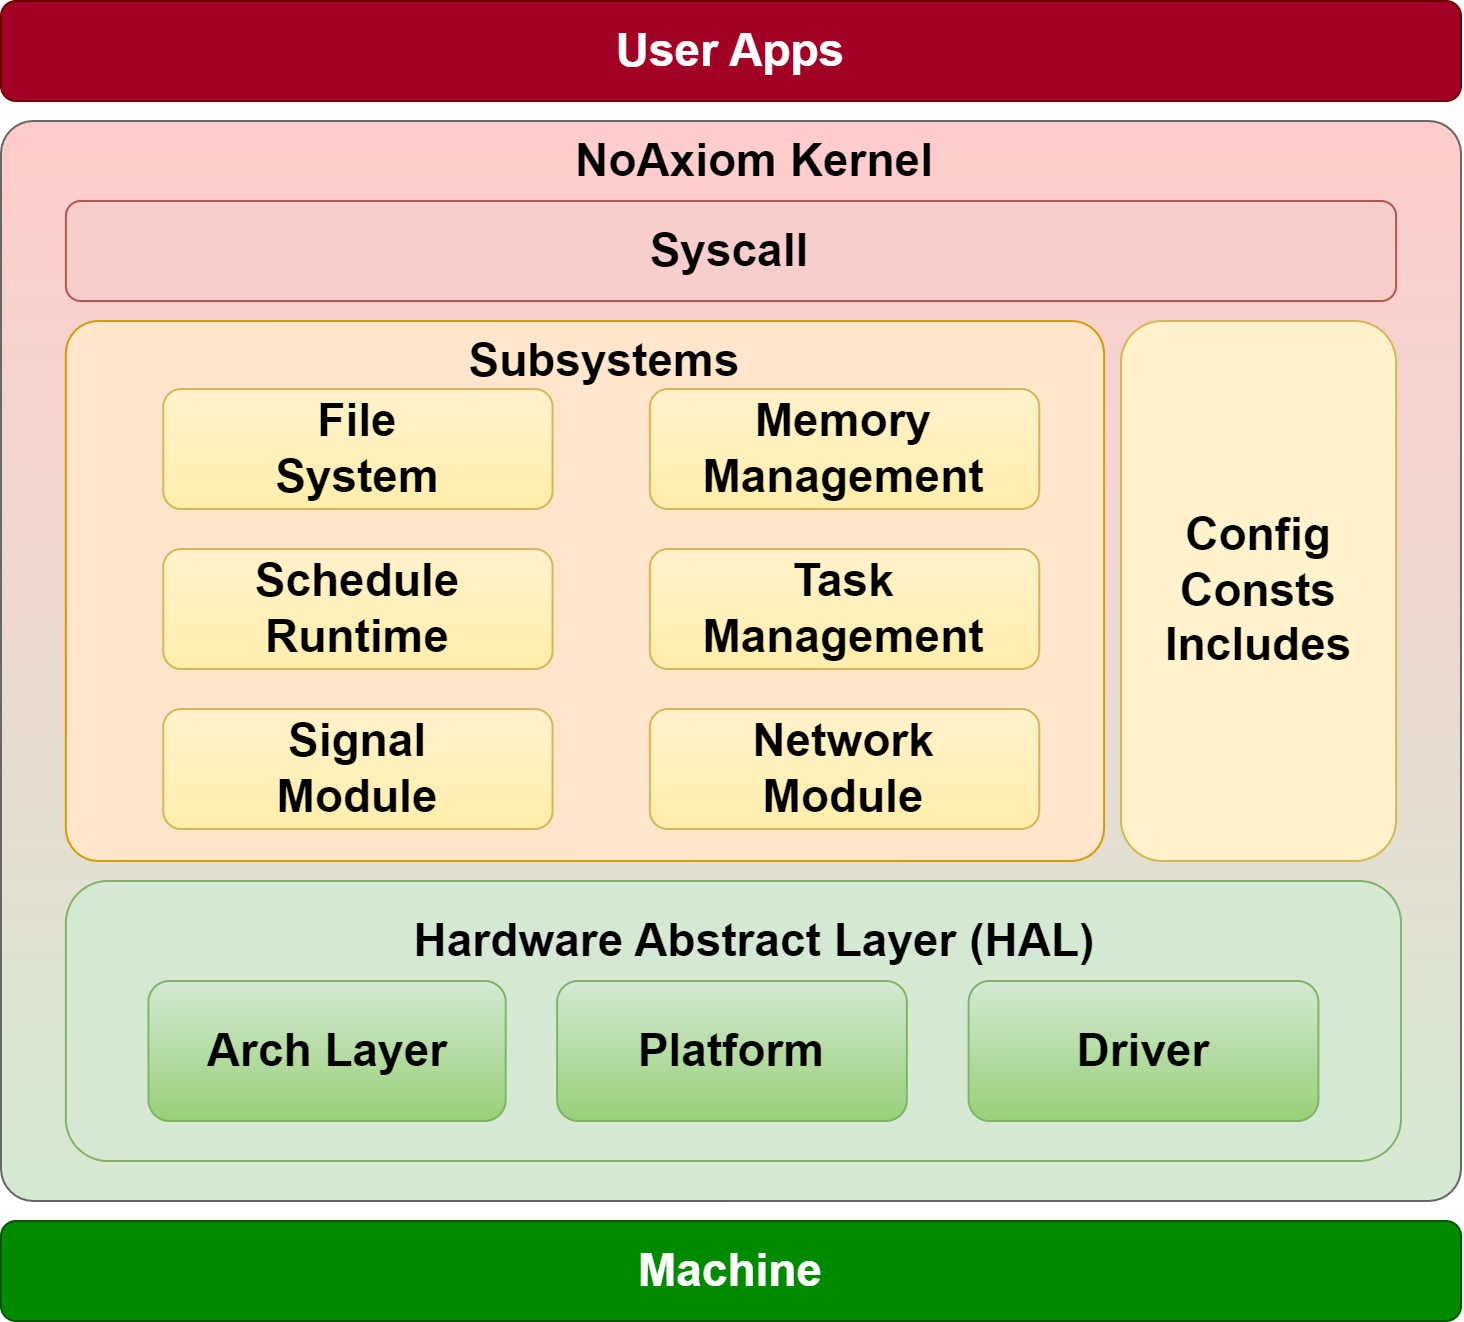
\includegraphics[width=0.85\linewidth]{assets/brief/noaxiom_structure.drawio.png}
    \caption{NoAxiom OS 整体架构}
    \label{fig:noaxiom_structure}
\end{figure}

更具体地,NoAxiom自底向上地将其架构分为如下四个层次:

\ding{226}\quad \textbf{机器层 / Machine Layer}

我们的目标是构建一个能够运行于多平台、多架构上的操作系统。我们的内核需要运行于RISC-V64架构和LoongArch64架构,且需要考虑到同时运行于QEMU虚拟机平台与物理上板平台。这些平台与架构均被归于机器层(Machine Layer),将会在上层的硬件抽象层中被实现为统一的接口提供给内核子系统。

\ding{226}\quad \textbf{硬件抽象层 / Hardware Abstraction Layer (HAL)}

硬件抽象层用于统一机器层的复杂环境,并向上层内核提供统一的功能接口。内核子系统通过调用硬件抽象层内部的多个子模块,实现与底层机器环境的完全解耦。这一设计在大赛要求双架构运行的背景下发挥了重要作用,使得我们能够完全脱离底层架构进行开发,一定程度上减少了处理内核在不同架构/平台下运行带来的额外编码工作量。具体而言,硬件抽象层又细分为指令集架构抽象层\code{arch},平台抽象层\code{platform},内存抽象层\code{memory},驱动抽象层\code{driver}等子模块,下面是详细描述。

\begin{enumerate}
    \item \textbf{指令集架构抽象层}:我们基于对LoongArch和RISC-V架构的了解,将所有受指令集架构影响的函数调用、类型定义、常量定义均视为同一对象\code{Arch}的\code{trait}子类,并将所有架构相关的实现放置于\code{lib/arch}库当中提供给所有上层子模块使用。借此内核实现了指令集架构上的解耦。
    \item \textbf{平台抽象层}:为了同时运行于虚拟机平台与物理上板环境,我们构建了平台抽象层用于进行平台与内核的解耦。具体而言,平台抽象层会根据编译时给定的平台与架构,向上提供统一的常量定义接口,从而实现内核与运行平台的完全解耦。
    \item \textbf{内存抽象层}:内存初始化布局会受到硬件平台的影响,同时驱动抽象层也需要依赖于物理页帧分配、虚实地址等功能,因此我们创建了内存抽象层向上提供统一的访存接口。本层次仅用于平台相关的内存初始化,以及架构、平台相关的内存抽象,真正的内存管理仍然由上层内核维护。
    \item \textbf{驱动抽象层}:在操作系统启动时,驱动抽象层会进行\textbf{自动的设备嗅探},读取设备树,并且自动嗅探挂载于不同总线上的设备信息,并且注册相应驱动,供上层内核使用。特别的,对于RISC-V架构,我们还会配置PLIC(Platform-Level Interrupt Controller),为需要中断的设备注册中断,并提供相应的中断处理例程。实现了内核与下层具体物理设备的解耦。
\end{enumerate}

\ding{226}\quad \textbf{内核实现层 / Kernel Implementation Layer}

内核实现层基于下层硬件抽象层的统一接口,使用统一的逻辑实现各类子模块的具体功能,并向用户提供完整的系统调用支持。除了细分的子模块外,我们与大多数操作系统一样,创建了统一的系统调用接口,用于统合操作系统内核提供的各个子模块的具体功能,并通过相关系统规范向用户提供统一的系统调用服务。

具体而言,内核实现层细分为以下若干子模块:

\begin{enumerate}
    \item \textbf{进程管理子模块}:进程管理子模块通过提供进程控制块与若干类型的任务管理器,向其他子模块提供基本的进程信息维护功能。
    \item \textbf{任务调度子模块}:任务调度子模块借助Rust的无栈协程语法,维护了分时多任务的异步调度器,实现了任务执行的全流程异步维护。
    \item \textbf{文件系统子模块}:文件系统子模块通过统一的VFS接口,向下统合多种不同的文件系统类型,向上提供统一的文件访问行为抽象;此外,文件系统结合无栈协程异步让权机制,实现了\textbf{耗时行为的异步调度},以及\textbf{异步的I/O多路复用}。
    \item \textbf{信号子模块}:信号子模块通过维护进程控制块中的信号信息,实现了不同进程之间的异步通信。
    \item \textbf{内存管理子模块}:内存管理子模块向其他模块提供统一的内存管理接口,并通过基于硬件抽象层提供的异常检查,用户提供精确的异常指针检查机制与懒分配让权机制。
    \item \textbf{时间管理子模块}:时间管理子模块通过设置若干时钟管理器,实现了可靠的时钟计时功能。
    \item \textbf{网络子模块}:网络子模块实现了TCP和UDP两种套接字API,支持IPv4和IPv6地址,在无栈协程架构下,实现了高并发下的准确高效的网络传输。
\end{enumerate}

\ding{226}\quad \textbf{用户应用层 / User Application Layer}

用户应用层基于内核提供的系统调用接口实现多种功能的用户程序。特别地,我们的内核内嵌了一个初始进程的elf文件用于进行用户程序的初始执行过程。赛事官方提供的测例均运行于这一层。

\subsection{系统完成情况}
截至目前,本系统共实现112条系统调用,涵盖了\textbf{文件系统、IO、网络、进程管理、信号处理、内存管理、调度管理、时间管理}等各类系统调用类型。能够运行赛事官方提供的除ltp部分测试点以外的全部测例。

NoAxiom在多个子模块均取得了较为明显的技术突破。截至目前,NoAxiom的具体子模块完成情况如\autoref{table:system-complete}所示。

% \linespread{1}
\begin{table}[H]
\centering
\caption{NoAxiom系统子模块完成情况}
\label{table:system-complete}
\begin{tabular}{p{3cm} p{9cm}}\toprule
    \textbf{子模块}& \textbf{实现情况}\\\toprule
    进程管理&\parbox{9cm}{
        统一的进程资源抽象\newline
        \textbf{细粒度}共享资源}
    \\\midrule
    
    内存管理&\parbox{9cm}{
        内核与用户地址空间共享\newline
        \textbf{懒分配与写时复制}检查\newline
        用户指针\textbf{合法性}的快速检查\newline
        文件映射懒分配的完整\textbf{异步让权}
    }\\\midrule
    
    文件系统&\parbox{9cm}{
        实现类Linux的\textbf{VFS虚拟文件系统}\newline
        支持管道、套接字及各类虚拟文件的挂载\newline
        支持\textbf{异步}EXT4、FAT32文件系统\newline
        为耗时读写操作实现了\textbf{异步让权}\newline
        实现了高效的\textbf{页缓存}加速文件读写\newline
        支持基于异步让权的\textbf{I/O多路复用}
    }\\\midrule
    
    任务调度&\parbox{9cm}{
        使用实现完整的\textbf{分时多任务异步}调度\newline
        使用统一的调度器特性抽象管理\textbf{多种调度器}\newline
        通过调度实体实现\textbf{任务优先级}
    }\\\midrule
    
    信号系统&\parbox{9cm}{
        实现信号系统维护\newline
        支持\textbf{可被信号中断}的系统调用
    }\\\midrule
    
    硬件抽象层&\parbox{9cm}{
        \textbf{自主}实现RISC-V64和LoongArch64\textbf{双架构支持}\newline
        \textbf{自主}实现与内核\textbf{统一解耦}的顶层硬件抽象接口\newline
        \textbf{自主}实现\textbf{访存}模块的架构解耦\newline
        \textbf{自主}实现\textbf{中断异常}处理的架构解耦
    }\\\midrule

    设备驱动&\parbox{9cm}{
        实现不同架构下\textbf{多总线的设备嗅探}\newline
        \textbf{自主}实现基于外部\textbf{中断}的\textbf{异步块设备驱动}\newline
        为块设备驱动实现\textbf{异步块缓存}
    }\\\midrule
    
    网络模块& \parbox{9cm}{
        支持TCP和UDP套接字\newline
        支持Ipv4与Ipv6协议\newline
        实现\textbf{端口复用}\newline
        支持等待时\textbf{异步让权}
    }\\\bottomrule
\end{tabular}
\end{table}
% \linespread{\defaultlinespread}

\newpage
\section{任务调度}
\subsection{无栈协程特性}

Rust语言于2019年推出了基于\code{async / await}关键字的无栈协程支持,简化了异步函数状态机的创建与维护过程,标志着Rust正式进入协程时代。而我们的内核也大量使用了这一语法特性,借助无栈协程实现了完整的异步让权机制。

\subsubsection{Rust的异步语法支持}

在Rust语言中,无栈协程底层由\code{Future}特性进行实现,其内部维护了一个无栈协程异步函数状态机,并通过调用\code{Future::poll()}方法进行异步函数的轮询操作。对应代码如下:

\begin{lstlisting}
pub trait Future {
    type Output;
    fn poll (
        self: Pin<&mut Self>, cx: &mut Context<'_>
    ) -> Poll<Self::Output>;
}
\end{lstlisting}

上述代码中涉及若干关键对象,下面是它们的具体含义及解释:

\begin{enumerate}
    \item \code{trait Future}:它是无栈协程中所有异步操作的上层抽象,当调用\code{Future::poll()}的时候,当前异步操作会尝试推动其进展,并返回其执行状态。
    \item \code{enum Poll<T>}:异步操作的返回值,用于指示当前异步操作的进展。
    \begin{itemize}
        \item \code{Poll::Pending}:表示当前异步操作仍未准备完毕,需要再次轮询。
        \item \code{Poll::Ready(val)}:表示当前异步操作已经完成,并会附带准备完毕的返回数据。
    \end{itemize}
    \item \code{Pin<Self>}:\code{poll()}方法中将当前对象包裹在\code{Pin}指针当中,该指针确保了其指向的对象位于固定的内存位置,不会被移动,这主要用于防止\code{Future}当中自引用导致的指针错误。
    \item \code{Context}:其内部支持了上下文相关信息,如唤醒器\code{Waker}等信息的保存。它允许\code{Future}在返回\code{Pending}时在运行时内保存间接指向其执行上下文的指针,从而在反应器感知到对应事件时,唤醒挂起的任务并将其重新加入到执行器中。
\end{enumerate}

而Rust中的\code{async / await}关键字是\code{Future}的语法糖,当一个函数被标记为\code{async}的时候,编译器会将其视作一个\code{Future}对象,并按照其内部的\code{.await}关键字排布,将其拆分为若干个子\code{Future}对象。

在执行异步函数时,程序会在堆空间上分配当前\code{Future}所需的数据空间,从而创建出无栈协程状态机。当执行器对于\code{async}函数生成的\code{Future}对象进行轮询的时候,其内部会按照当前状态机的执行状态,对当前执行到的子\code{Future}对象进行\code{poll}方法的调用,从而实现异步函数执行上下文的维护。

\subsubsection{异步运行时} \label{sec:async_runtime}

在Rust语言中,异步运行时(Async Runtime)由执行器(Executor),反应器(Reactor),调度器(Scheduler)等组件组成,这些组件共同构成了无栈协程运行时(Rust Stackless Coroutine Runtime)。我们的操作系统完全基于Rust无栈协程语法构建,所有任务最终均在运行时上完成执行。

下面对无栈协程运行时内部组件进行详细的描述。

\begin{itemize}
    \item \textbf{执行器}(Executor):执行器组件用于提供异步函数在同步控制流中的\textbf{执行}功能,当执行器执行一个任务时,任务将处于执行态。
    
    Rust的\code{Future}是惰性的,在调用其\code{poll()}方法前,它不会真正被驱动执行。Rust语言规定了\code{.await}只能在一个异步函数\code{async fn}内被调用,因此对于最外层的异步函数,需要一个执行器用于在同步控制流当中启动该无栈协程异步函数。在NoAxiom当中,我们选择了基于\code{async_task}\footnote{https://github.com/smol-rs/async-task}外部库构建无栈协程执行器。该外部库会通过\code{AtomicUsize}原子访存对于任务的调度状态进行内部维护,保证任务对象在重复唤醒时的唯一性。
    
    \item \textbf{反应器}(Reactor):反应器用于保存异步执行时\textbf{挂起}的任务,并在对应事件完成时重新唤醒对应任务。当任务被保存在反应器内时,它将处于挂起状态。
    
    在一个设计完备的异步系统当中,当一个\code{Future}对应的异步执行任务尚未完成时,系统应当将当前任务切出,并将任务保存在反应器当中。反应器会通过中断或轮询等方式监听对应的事件,当检测到对应的异步任务被标记为执行完成时,再重新唤醒对应的任务使其继续执行。

    在NoAxiom当中,反应器并不对应一个特定组件,而是通过中断处理例程、时间管理例程等形式分布在内核中的各个组件内部。

    \item \textbf{调度器}(Scheduler):调度器用于保存已被唤醒、\textbf{可运行}的任务。它可以向执行器提供可执行任务,也可以响应反应器唤醒的任务。当任务位于调度器内时,它将处于可执行态。
    
    在部分Rust无栈协程设计当中,对于执行器和调度器并没有进行良好区分。但为了设计解耦,NoAxiom选择将调度器与执行器严格区分以独立解耦内核调度过程,并构建了良好的调度器抽象,以实现多种任务调度功能。
    
\end{itemize}

异步运行时的内部组件构成了从调度器到执行器,执行器到反应器,反应器再唤醒回到调度器的完整执行循环。其执行循环如\autoref{fig:async_runtime}所示,其中描述了各个组件及对应的任务执行状态,可以参考 \ref{sec:task_status} 中的任务状态切换查看其具体对应关系。

\begin{figure}[H]
    \centering
    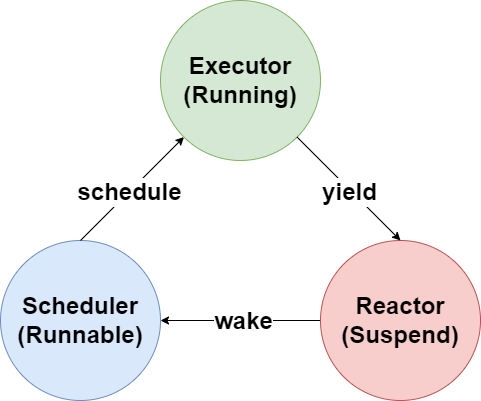
\includegraphics[width=0.4\linewidth]{assets//sched/async_runtime.drawio.png}
    \caption{异步运行时组件间关系}
    \label{fig:async_runtime}
\end{figure}

\subsection{模块化调度抽象}

我们的操作系统基于轻量级异步执行器开源库\href{https://github.com/smol-rs/async-task}{async-task}构建了独属于我们操作系统的模块化调度器,实现了良好的调度器抽象,并针对不同调度场景设计了特定的调度器进行灵活调度。

\begin{figure}[H]
    \centering
    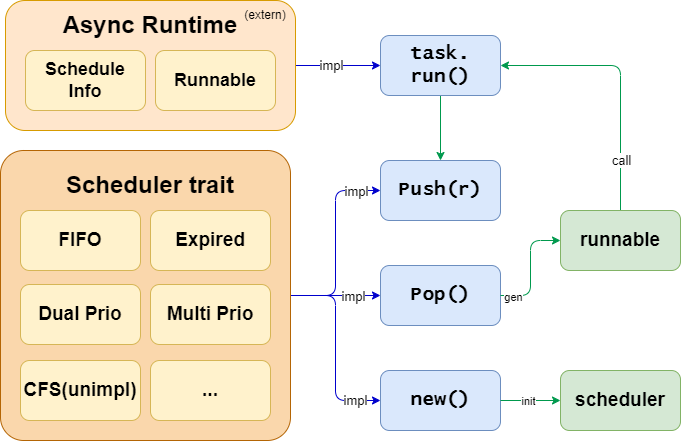
\includegraphics[width=0.8\linewidth]{assets//sched/scheduler_types.drawio.png}
    \caption{模块化调度器设计}
    \label{fig:async_runtime}
\end{figure}

\subsubsection{调度器特性抽象}

根据我们在 \ref{sec:async_runtime} 中对于异步运行时的设计,在NoAxiom中,调度器最终被抽象为独立、统一的特性对象\code{trait Scheduler<R>}。除了用于初始化的\code{Scheduler::new()}\footnote{由于实现较为简单,下文中我们将省略展示的代码中对该方法的实现}之外,\code{Scheduler}中定义了两个关键方法\code{push()}和\code{pop()},分别用于反应器中的\code{Waker}唤醒与执行器中的可执行任务获取过程。

具体函数定义如下所示。

\begin{lstlisting}
/// NoAxiom/kernel/src/sched/vsched.rs
pub trait Scheduler<R> {
    fn new() -> Self;
    fn push(&mut self, runnable: Runnable<R>, info: ScheduleInfo);
    fn pop(&mut self) -> Option<Runnable<R>>;
}
\end{lstlisting}

基于该调度器特性抽象,我们可以设计出多种适用于不同调度场景的调度器,并向外暴露统一的接口给运行时以进行调度。



\subsubsection{运行时特性抽象}

在NoAxiom的设计当中,运行时\code{Runtime}用于统合执行器、调度器、反应器三者的功能,并向内部组件提供顶层的接口支持。其中具体成员方法及其含义如下:

\begin{itemize}
    \item \code{run()}方法:用于调用执行器进行单个任务的执行。
    \item \code{schedule()}方法:用于反应器访问调度器插入可执行任务。
    \item \code{spawn()}方法:用于将异步函数与任务控制块打包为统一的\code{Runnable}对象投入调度中。
\end{itemize}

\begin{lstlisting}
pub trait Runtime<T, R>
where
    T: Scheduler<R>,
{
    fn new() -> Self;
    fn run(&self);
    fn schedule(&self, runnable: Runnable<R>, info: ScheduleInfo);
    fn spawn<F>(self: &'static Self, future: F, task: Option<&Arc<Task>>)
    where F: Future<Output: Send + 'static> + Send + 'static;
}
\end{lstlisting}

通过提供运行时特性抽象,我们可以根据实际运行的平台选定特定的运行策略,并为运行时选定具体的底层调度器,以实现灵活的调度策略选择。

\subsection{多种调度器设计}

基于\code{Scheduler<R>}特性,我们可以方便的设计出多种底层调度器实现。下面将列举NoAxiom系统中的具体调度器实现。

\subsubsection{先入先出调度}

先入先出调度(First In First Out, FIFO)是一种常见且朴素的调度策略,通过对于所有任务的轮询过程避免了因调度优先级导致的任务饥饿情况。在NoAxiom当中,我们选择使用全局自旋锁+双端队列维护FIFO调度队列。具体代码如下。

\begin{lstlisting}
/// NoAxiom/kernel/src/sched/scheduler.rs
struct FifoScheduler {
    queue: VecDeque<Runnable<Info>>,
}
impl Scheduler<Info> for FifoScheduler {
    fn push(&mut self, runnable: Runnable<Info>, _: async_task::ScheduleInfo) {
        self.queue.push_back(runnable);
    }
    fn pop(&mut self) -> Option<Runnable<Info>> {
        self.queue.pop_front()
    }
}
\end{lstlisting}

\subsubsection{双优先级调度}

在常规的调度过程中,有两类调度行为较为常见:

\begin{itemize}
    \item 让权(yield):主要用于轮询行为,程序通过调用\code{yield_now().await}主动让出当前任务执行权,此时的任务应当被重新加入到调度队列末尾,等待后续任务执行完毕后再次进行轮询。
    \item 挂起-唤醒(suspend-wake):主要发生在异步操作的执行过程当中,如块设备访问、管道I/O等。该调度行为在唤醒时应当得到尽可能早的响应,以降低系统响应延迟。
\end{itemize}

以上两类调度行为对于调度队列的维护方式要求完全相反,让权行为要求任务尽可能晚地得到下一次调度,而挂起后唤醒行为要求任务尽可能早地得到唤醒后的响应。因此我们设计了双优先级的调度队列,其中\code{idle}调度队列专门用于放置通过让权行为压入的任务,\code{normal}调度队列用于放置挂起后唤醒的任务。在调度时会优先选择\code{normal}队列中的任务进行执行。

\begin{lstlisting}
pub struct DualPrioScheduler {
    normal: FifoScheduler,
    idle: FifoScheduler,
}
impl Scheduler<Info> for DualPrioScheduler {
    fn push(&mut self, runnable: Runnable<Info>, info: async_task::ScheduleInfo) {
        match info.woken_while_running {
            true => self.idle.push(runnable, info),
            false => self.normal.push(runnable, info),
        }
    }
    fn pop(&mut self) -> Option<Runnable<Info>> {
        if let Some(runnable) = self.normal.pop() {
            return Some(runnable);
        }
        self.idle.pop()
    }
}
\end{lstlisting}

\subsubsection{分步队列调度}

上节中双优先级队列调度方式有一个明显的缺陷:当\code{normal}队列中存在频繁的唤醒行为时,\code{idle}队列会因为调度优先级原因一直无法得到执行,从而导致严重的饥饿情况。当\code{normal}队列中的任务依赖于\code{idle}队列中的任务发送的信息时,甚至会导致调度层面上的死锁。

由此,我们借鉴了Linux中的MLFQ调度算法与FSCAN调度算法,设计了较为简易的分步多级调度队列,通过维护\code{current}队列和\code{expired}队列,实现对于优先级队列的轮询式调度。具体而言,调度队列在执行\code{push()}方法的时候,并不会将任务插入到当前的\code{current}队列当中,而是将新的任务插入到\code{expired}队列当中,直到\code{current}队列中所有任务执行完毕,再交换两个队列实现轮询式调度。

该调度设计良好地避免了任务饥饿,同时兼顾了任务的调度优先级。

\begin{lstlisting}
type ExpiredSchedulerInnerImpl = DualPrioScheduler;
pub struct ExpiredScheduler {
    current: SyncUnsafeCell<ExpiredSchedulerInnerImpl>,
    expire: SyncUnsafeCell<ExpiredSchedulerInnerImpl>,
}
impl ExpiredScheduler {
    fn switch_expire(&mut self) {
        core::mem::swap(&mut self.current, &mut self.expire);
    }
}
impl Scheduler<Info> for ExpiredScheduler {
    fn push(&mut self, runnable: Runnable<Info>, info: async_task::ScheduleInfo) {
        self.expire.as_ref_mut().push(runnable, info);
    }
    fn pop(&mut self) -> Option<Runnable<Info>> {
        let current = self.current.as_ref_mut();
        let res = current.pop();
        if let None = res.as_ref() {
            self.switch_expire();
            self.current.as_ref_mut().pop()
        } else {
            res
        }
    }
}
\end{lstlisting}

\subsubsection{多级调度}

部分测例(如:cyclictest)对于操作系统调度实时性提出了要求。而上节中的双优先级+分步队列调度方式在避免饥饿的同时,也放弃了对于唤醒的高优先级任务的快速响应能力。因此其只适用于常规任务的维护,无法提供良好的实时任务支持。为了实现实时任务的快速响应,我们必须在常规任务队列的基础上再创建额外的实时调度队列。

目前NoAxiom只在多级队列中维护了单一优先级的实时调度队列,其内部维护了一个FIFO调度队列。当对多级调度队列进行插入操作时,调度器会通过共享裸指针的方式获取当前待调度任务的调度实体\code{SchedEntity}数据以获取其调度优先级\code{SchedPrio},并通过优先级决定最终插入的队列;当对多级队列进行弹出操作时,调度器会优先弹出实时队列当中的任务,从而实现尽可能早的实时任务响应行为。

% 关于具体的实时性优化效果,详见 \ref{sec:perf_realtime} 中描述。

\begin{lstlisting}
type RealTimeSchedulerImpl = FifoScheduler;
type NormalSchedulerImpl = ExpiredScheduler;
#[repr(align(64))]
pub struct MultiLevelScheduler {
    realtime: RealTimeSchedulerImpl,
    normal: NormalSchedulerImpl,
}
impl Scheduler<Info> for MultiLevelScheduler {
    fn push(&mut self, runnable: Runnable<Info>, info: async_task::ScheduleInfo) {
        let entity = runnable.metadata().sched_entity();
        if let Some(entity) = entity {
            match entity.sched_prio {
                SchedPrio::RealTime(_) => self.realtime.push(runnable, info),
                _ => self.normal.push(runnable, info),
            }
        } else {
            self.realtime.push(runnable, info);
        }
    }
    fn pop(&mut self) -> Option<Runnable<Info>> {
        if let Some(runnable) = self.realtime.pop() {
            return Some(runnable);
        }
        self.normal.pop()
    }
}
\end{lstlisting}

\subsection{调度信息维护}

\subsubsection{调度实体}

为了方便在调度器与任务控制块之间共享调度信息,我们使用调度实体\code{SchedEntity}进行调度相关信息的维护。目前,\code{SchedEntity}内维护了任务的调度优先级\code{sched_prio}、CPU掩码\code{cpu_mask}、时间统计信息\code{time_stat}等信息,其中就包含了涉及实时性调度的关键成员\code{sched_prio}。

\begin{lstlisting}
/// NoAxiom/kernel/src/sched/sched_entity.rs
pub struct SchedEntity {
    pub sched_prio: SchedPrio, // scheduling priority
    pub time_stat: TimeInfo,   // task time
    pub cpu_mask: CpuMask,     // cpu mask
}
\end{lstlisting}

在任务控制块中我们将调度实体设置为了线程独属的数据,并使用\code{SyncUnsafeCell}进行维护。但Rust并不允许\code{SyncUnsafeCell::get()}获得的裸指针在调度器与任务控制块之间直接共享,因此我们对调度实体进行了一层\code{Sync}包装,并通过\code{SchedMetadata}进行数据的传递。

\begin{lstlisting}
pub struct SchedMetadata {
    ptr: *mut SchedEntity,
    tid: usize,
}
unsafe impl Sync for SchedMetadata {}
unsafe impl Send for SchedMetadata {}
\end{lstlisting}

\subsubsection{调度优先级}

与上节中的描述一致,我们将任务的调度优先级分为三种:

\begin{itemize}
    \item 实时优先级\code{RealTime(usize)}:用于指示特殊的实时任务调度,其中预留了实时任务内部优先级,以应对未来可能的扩展。
    \item 普通优先级\code{Normal}:用于常规执行中因异步操作让权后唤醒的任务,大多数任务均处于这一调度优先级。
    \item 闲置优先级\code{IdlePrio}:我们参照BFS和MuQSS的设计,为主动让权的进程额外创立了这个调度优先级。由于主动让权的进程通常执行的是轮询行为,其执行通常对时间不敏感,因此将会在执行完普通任务后再进行该优先级任务的执行。
\end{itemize}

\begin{lstlisting}
pub enum SchedPrio {
    RealTime(usize),
    Normal,
    IdlePrio,
}
\end{lstlisting}

\subsection{异步运行时实现}

目前而言,NoAxiom的异步运行时内部仅维护了一个顶层的多级队列调度器,运行时将通过调用其内部调度器的各类方法,联合外部执行器依赖库创建任务,进一步实现各类运行时功能。

\begin{lstlisting}
/// NoAxiom/kernel/src/sched/runtime.rs
type SchedulerImpl = MultiLevelScheduler;
pub struct SimpleRuntime {
    scheduler: SpinLock<SchedulerImpl>,
}
\end{lstlisting}

\subsubsection{异步任务的生成}

我们通过\code{Runtime::spawn()}方法将一个\code{Future}异步函数对象与\nameref{sec:task_control_block}\code{Arc<Task>}打包为执行器库中的\code{Runnable}对象进行调度。具体而言,当生成一个新任务时,将通过调用\code{async_task}库中的\code{spawn()}方法以获取生成器生成的任务对象\code{(runnable, handle)},并调用\code{runnable.schedule()}方法将其投入调度队列中。

我们使用的外部执行器依赖库\code{async_task}中默认关闭了对于其调度对象\code{Runnable<T = ()>}的额外元信息维护。想要通过\code{SchedMetadata}在执行器环境中共享调度信息,应当在创建异步任务时额外调用\code{async_task::Builder::new().metadata()}中的构建方法以携带额外的元信息。此后,即可在调度器中通过调用\code{Runnable::metadata()}方法获取到构建的元信息了。

\begin{lstlisting}
/// NoAxiom/kernel/src/sched/runtime.rs
impl Runtime<SchedulerImpl, Info> for SimpleRuntime {
    fn spawn<F>(self: &'static Self, future: F, task: Option<&Arc<Task>>)
    where
        F: core::future::Future<Output: Send + 'static> + Send + 'static,
    {
        let metadata = task
            .map(|task| SchedMetadata::from_task(task))
            .unwrap_or_else(SchedMetadata::default);
        let (runnable, handle) = Builder::new().metadata(metadata).spawn(
            move |_| future,
            WithInfo(move |runnable, info| self.schedule(runnable, info)),
        );
        runnable.schedule();
        handle.detach();
    }
}
\end{lstlisting}

\subsubsection{异步任务的调度与运行}

我们通过\code{Runtime::schedule()}进行单个任务的调度申请,该方法通过调用\code{Scheduler::push()}方法实现向调度器中添加一个新的可执行任务的功能。

我们通过\code{Runtime::run()}进行单个任务的单次执行,该函数会通过调用\code{Scheduler::pop()}函数获取一个待执行的任务,并通过调用异步执行器的\code{Runnable::run()}方法在同步控制流中实现单次异步函数的轮询行为。

\begin{lstlisting}
impl Runtime<SchedulerImpl, Info> for SimpleRuntime {
    fn run(&self) {
        let runnable = self.scheduler.lock().pop();
        if let Some(runnable) = runnable {
            runnable.run();
        }
    }
    fn schedule(&self, runnable: Runnable<Info>, info: async_task::ScheduleInfo) {
        self.scheduler.lock().push(runnable, info);
    }
}
\end{lstlisting}

我们的内核一旦初始化完成,就将持续访问运行时执行任务。该行为被包装为\code{run_task()}函数,作为最顶层的执行循环,实现运行时的不间断执行行为。

\begin{lstlisting}
#[no_mangle]
pub fn run_tasks() -> ! {
    loop {
        timer_handler();
        RUNTIME.run();
    }
}
\end{lstlisting}

\newpage
\section{进程管理}
\subsection{任务控制块} \label{sec:task_control_block}

在操作系统中,进程是资源分配的单位,其拥有独立的资源空间。而线程是共享进程资源的执行单元,作为属于某一进程下的活动对象参与执行。在Linux系统中,进程和线程被统一表示为轻量级进程(Lightweight Process, LWP),并通过统一的任务控制块进行进程与线程资源的管理。在NoAxiom当中,我们延续了这一设计,将任务抽象为\code{Task}对象,从而实现了对于进程和线程的统一管理。

\subsubsection{资源访问属性}

在任务控制块中,资源的访问属性尤为重要,错误的访问级别会导致锁和裸指针的错误使用,进而导致频繁的资源竞争或多核间数据一致性问题。为了清晰表示任务资源的访问属性,在设计任务控制块的过程当中,我们将任务内部资源按照\textbf{是否共享}、\textbf{是否可访问}、\textbf{是否可变}大致分为下面四种类型。

\begin{lstlisting}
/// shared between threads
type SharedMut<T> = Arc<SpinLock<T>>;

/// mutable resources mostly used in current thread
/// it could be accessed by other threads through process manager
/// so protect it with spinlock
type Mutable<T> = SpinLock<T>;

/// only used in current thread, mutable resources without lock
/// SAFETY: these resources won't be shared with other threads
type ThreadOnly<T> = SyncUnsafeCell<T>;

/// read-only resources, could be shared safely through threads
type Immutable<T> = T;
\end{lstlisting}

上述定义的具体解释如\autoref{table:task-access-disign}所示。

\begin{table}[h!]
\centering
\caption{进程内部成员访问属性定义}
\label{table:task-access-disign}
\begin{tabular}{l l l l}\toprule
    \textbf{字段名称}& \textbf{访问属性}& \textbf{具体含义}& \textbf{具体维护策略}\\\midrule
    \code{SharedMut<T>}& 共享、可变& 线程间共享资源& 使用引用计数和自旋锁维护\\
    \code{Mutable<T>}& 可访问、可变& 可被管理器访问的独占资源& 使用自旋锁维护\\
    \code{ThreadOnly<T>}& 独享、可变& 仅当前线程可访问的独占资源& 使用裸指针维护\\
    \code{Immutable<T>}& 不可变& 只读数据,可被任意读取& 直接保存在控制块中\\\bottomrule
\end{tabular}
\end{table}

\subsubsection{任务控制块}

基于以上访问权限设计,我们可以给出任务控制块的具体内部成员定义,用于记录任务相关的所有信息,如下所示。其具体字段的含义在 \autoref{table:task-control-block-members} 中给出。

\begin{lstlisting}
/// NoAxiom/kernel/src/task/task.rs
#[repr(C, align(64))]
pub struct Task {
    // mutable
    pcb: Mutable<PCB>, // task control block inner, protected by lock

    // thread only / once initialization
    tcb: ThreadOnly<TCB>,                  // thread control block
    cx: ThreadOnly<TaskContext>,           // trap context
    sched_entity: ThreadOnly<SchedEntity>, // sched entity for the task
    waker: Once<Waker>,                    // waker for the task
    ucx: ThreadOnly<UserPtr<UContext>>,    // ucontext for the task

    // immutable
    tid: Immutable<TidTracer>,              // task id, with lifetime holded
    tgid: Immutable<TGID>,                  // task group id, aka pid
    tg_leader: Immutable<Once<Weak<Task>>>, // thread group leader

    // shared
    fd_table: SharedMut<FdTable>,         // file descriptor table
    cwd: SharedMut<Path>,                 // current work directory
    sa_list: SharedMut<SigActionList>,    // signal action list, saves signal handler
    memory_set: SharedMut<MemorySet>,     // memory set for the task
    thread_group: SharedMut<ThreadGroup>, // thread group
    pgid: Arc<AtomicUsize>,               // process group id
    futex: SharedMut<FutexQueue>,         // futex wait queue
    itimer: SharedMut<ITimerManager>,     // interval timer
}
\end{lstlisting}

有关任务控制块内部关键成员的说明如下。

\begin{enumerate}[leftmargin=2\parindent]
    \item 任务ID:我们使用全局的TID分配器进行任务ID的原子性分配,并基于RAII的思想,通过\code{TidTracer}将其生命周期与任务绑定。TID将作为任务的唯一标识参与各类管理器的访问中。
    
    \item 进程控制块:为了保证原子性地维护进程间关系以及信号信息,我们选择将所有进程间父子关系和信号控制信息全部放置在进程控制块\code{PCB}当中进行维护,并使用自旋锁对其访问原子性进行保护。下面是\code{PCB}的成员,其具体字段含义在 \autoref{table:process-control-block-members} 中给出。
    
    \item 共享资源:以\code{clone(2)}\footnote{https://www.man7.org/linux/man-pages/man2/clone.2.html}为代表的若干系统调用会通过设置\code{CloneFlags}的方式,规定进程在复制时的资源共享情况。这些资源包括:\code{fd_table}, \code{cwd}, \code{sa_list}, \code{memory_set}, \code{thread_group}, \code{pgid}, \code{futex}, \code{itimer}等。通过这些共享资源,当前线程可以与其他兄弟进程或线程共享资源,从而实现更高效的资源利用。为了维护共享资源,我们使用引用计数指针\code{Arc<T>}对其进行生命周期维护,并使用自旋锁\code{SpinLock}维护修改的原子性。\code{SpinLock}\footnote{https://github.com/os-module/kernel-sync}是一种自旋锁,通过我们自定义的\code{NoIrqLockAction}机制,实现持有锁期间的中断使能关闭机制,因而它适用于实现短时锁定时的原子性保证,尤其是内核中对延迟敏感的部分。而共享引用计数\code{Arc}允许线程之间所有权的共享,在引用计数变为0时数据才会被释放,实现了共享资源生命周期的维护。
    
    \item 独占资源:我们保证当前任务独占资源不会被其他任务以任何形式单独访问,因此这些资源不需要额外的锁开销进行一致性维护,可以使用裸指针直接进行访问。由于裸指针包装器\code{UnsafeCell}未实现\code{Sync}属性,无法安全地在进程间传递,因此我们使用实现了\code{Sync}属性的\code{SyncUnsafeCell}绕过编译器检查,允许其在多线程环境下安全地传递。
    
    \item 资源访问:通过\code{Arc<SpinLock>}和\code{SyncUnsafeCell}的严格定义,任务控制块保护了共享数据访问原子性以实现线程安全,同时也保证了独占资源高效访问的高并发性,二者结合实现了并发情况下的高效性与正确性。
\end{enumerate}

\begin{table}[h!]
\centering
\caption{任务控制块成员定义}
\label{table:task-control-block-members}
\begin{tabular}{l l l}\toprule
    \textbf{字段名称}& \textbf{访问属性}& \textbf{具体含义}\\\midrule
    \code{pcb}& 可变& 进程控制块,用于维护进程信息原子性修改\\
    \code{tcb}& 独占& 线程控制块,用于维护其他线程独占信息\\
    \code{cx}& 独占& 任务上下文,保存任务的上下文信息\\
    \code{sched\_entity}& 独占& 调度实体,包含任务的调度信息\\
    \code{waker}& 独占& 唤醒器,用于异步任务唤醒\\
    \code{ucx}& 独占& 信号处理时保存的用户态上下文信息\\
    \code{tid}& 不可变& 任务ID,同时绑定了tid的生命周期\\
    \code{tgid}& 不可变& 线程组ID,也用作表示进程ID号\\
    \code{tg\_leader}& 不可变& 保存对线程组先导任务的弱引用\\
    \code{fd\_table}& 共享可变& 文件描述符表\\
    \code{cwd}& 共享可变& 当前工作目录\\
    \code{sa\_list}& 共享可变& 信号处理器列表\\
    \code{memory\_set}& 共享可变& 内存空间,保存任务的全部内存映射信息\\
    \code{thread\_group}& 共享可变& 线程组,维护当前线程组中的任务引用\\
    \code{pgid}& 共享可变& 进程组ID,使用原子操作维护可变性\\
    \code{futex}& 共享可变& Futex等待队列\\
    \code{itimer}& 共享可变& 间隔定时器管理器\\\bottomrule
\end{tabular}
\end{table}

\begin{table}[h!]
\centering
\caption{进程控制块成员定义}
\label{table:process-control-block-members}
\begin{tabular}{l l}\toprule
    \textbf{字段名称}& \textbf{具体含义}\\\midrule
    \code{status}& 任务状态,表示任务的当前状态\\
    \code{exit\_code}& 任务退出码,表示任务的退出状态\\
    \code{children}& 子任务列表,保存当前任务的子进程的强引用\\
    \code{parent}& 父任务引用,保存当前任务的父进程的弱引用\\
    \code{pending\_sigs}& 待处理信号,保存当前任务的待处理信号信息\\
    \code{sig\_stack}& 信号备用栈,保存信号处理时的备用栈信息\\
    \code{robust\_list}& 保存robust列表信息\\\bottomrule
\end{tabular}
\end{table}

\subsection{任务状态} \label{sec:task_status}

\subsubsection{任务状态转化关系}

我们在设计任务状态时,参考Linux的任务状态设计了以下若干任务状态,并将任务状态保存在\code{PCB::TaskStatus}当中,以自旋锁进行互斥访问。

任务状态转换如\autoref{fig:task_status}所示。

\begin{enumerate}
    \item \code{Running}:当前任务正在处于运行状态,正在被执行器执行中。
    \item \code{Runnable}:当前任务可运行但未被执行,存在于调度器中。
    \item \code{Suspend}:当前任务挂起,保存在反应器中等待外部事件唤醒。
    \item \code{Stopped}:当前任务被信号标记为暂停,检测到该状态后将挂起(Suspend)当前任务。
    \item \code{Terminated}:当前任务被exit等系统调用标记为退出。当任务检测到处于该状态后会执行任务退出处理例程并进入僵尸态(Zombie)。
    \item \code{Zombie}:当前任务执行完毕并进入僵尸态,等待父进程对其资源进行回收。
\end{enumerate}

\begin{figure}[H]
    \centering
    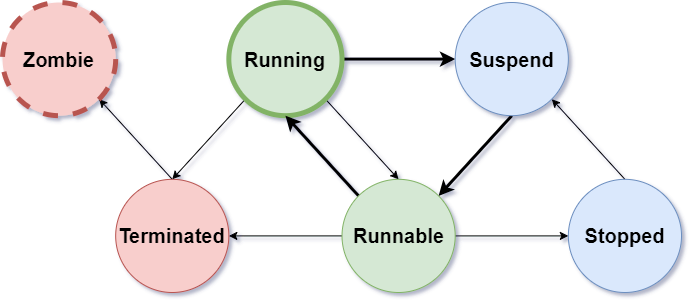
\includegraphics[width=0.7\linewidth]{assets/task/task_status.drawio.png}
    \caption{任务状态转换状态机}
    \label{fig:task_status}
\end{figure}

\subsubsection{调度相关状态简化设计}

在查看外部库async-task的过程当中,我们注意到:该外部库已经通过原子标志位维护了任务的运行(Running)、等待(Runnable)、挂起(Suspend)三个状态了。具体而言,该外部库会通过\code{Header}中的\code{state}成员进行原子访存,以此维护当前任务在调度方面的状态更新原子性。

\begin{lstlisting}
/// async-task/src/header.rs
pub(crate) struct Header<M> {
    /// Current state of the task.
    /// Contains flags representing the current state and the reference count.
    pub(crate) state: AtomicUsize,
}
\end{lstlisting}

例如,在执行\code{runnable.run()}将某个任务从等待态变为运行态的时候,该外部库会通过原子访存将\code{SCHEDULED}位重置,以通知运行时该任务可再次通过\code{runnable.schedule()}加入调度队列中。

\begin{lstlisting}
let state = (*raw.header).state.fetch_and(!SCHEDULED, Ordering::AcqRel);
\end{lstlisting}

因此在NoAxiom中,我们将常规的三种执行状态\code{Running}、\code{Runnable}、\code{Suspend}实际统一为\textbf{固定的\code{Normal}状态},而实际的执行状态则通过任务在运行时中保存的调度模块决定。有关具体保存的调度模块,详见\ref{sec:async_runtime}章节中的描述,其中\autoref{fig:async_runtime}详细描述了本章节中的对应状态转化图。

\subsection{任务间关系}

\subsubsection{进程间关系}

在操作系统中,进程通过\code{clone(2)}等系统调用创建子进程,以此构成进程之间的父子关系。当子进程退出时,为了保证进程资源的一致性,其占用的资源需要父进程帮助回收。具体而言,任务控制块的\code{pcb}中维护了进程的父子关系信息,通过持有子进程的强引用\code{children: Vec<Arc<Task>>}防止其提早析构,并持有父进程的弱引用\code{parent: Option<Weak<Task>>}便于临时获取父进程的任务控制块。

\subsubsection{线程间关系}

我们参照Linux中的设计,使用线程组(Thread Group)维护同一进程下的线程。进程组中将维护一个主线程,作为当前线程组的进程级任务,负责管理共享资源以及所有同一线程组下的线程级任务;而其余的所有任务均被视作线程,线程之间不存在父子关系,也不需要对进程资源的维护直接负责。当进程退出时,其他所有的线程都需要退出,并等待父进程回收其资源;当非主线程退出时,将会主动进行资源释放。线程组结构如\autoref{fig:thread_group_structure}所示。

\begin{figure}[H]
    \centering
    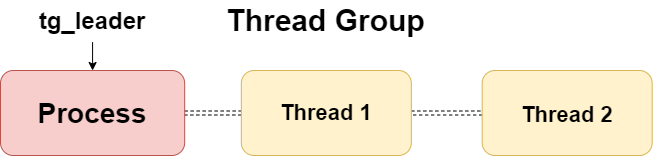
\includegraphics[width=0.5\linewidth]{assets//task/thread_group.drawio.png}
    \caption{线程组结构}
    \label{fig:thread_group_structure}
\end{figure}

具体而言,每个进程下的所有线程都会通过\code{Task::thread_group}共享同一个线程组。线程组内部维护了从任务号\code{tid}到任务控制块\code{Weak<Task>}的映射,用于线程组信息的快速访问与维护。此外,任务控制块内会额外维护一个主线程\code{tg_leader}用于代表整个进程,该主线程的任务号\code{tid}也将作为线程组号/进程号\code{tgid}保存在任务控制块中。通过访问线程组,可以较为便利地对同一进程下的所有线程信息进行读取和维护。

\begin{lstlisting}
pub struct ThreadGroup(pub BTreeMap<TID, Weak<Task>>);
impl ThreadGroup {
    pub const fn new() -> Self {
        Self(BTreeMap::new())
    }
    pub fn insert(&mut self, task: &Arc<Task>) {
        self.0.insert(task.tid(), Arc::downgrade(&task));
    }
    pub fn remove(&mut self, taskid: usize) {
        self.0.remove(&taskid);
    }
}
\end{lstlisting}

\subsubsection{任务管理器}

仅仅通过进程父子关系、线程组关系的维护并不足以实现完整的任务管理。我们参照Linux的设计,创建了任务管理器\code{TaskManager}用于实现全局的任务关系维护。与线程组类似,任务管理器将保存任务标识\code{tid}到任务控制块\code{Weak<Task>}的映射关系,以用于所有任务信息的快速访问与维护。

\begin{lstlisting}
/// NoAxiom/kernel/src/task/manager.rs
pub struct TaskManager(pub SpinLock<BTreeMap<TID, Weak<Task>>>);
pub static TASK_MANAGER: Lazy<TaskManager> = Lazy::new(|| TaskManager::new());
\end{lstlisting}

\subsubsection{进程组管理器}

在兼容于POSIX标准的操作系统中,进程组(Process group)是指一个或多个进程的集合。进程组被使用于控制信号的分配。对于一个进程组发出的的信号,会被个别递送到这个组群下的每个进程成员中。\footnote{https://en.wikipedia.org/wiki/Process\_group}NoAxiom严格遵循POSIX相关标准,对于进程组使用进程组管理器\code{ProcessGroupManager}进行维护。其内部通过维护同一进程组号\code{PGID}下的所有进程,实现某一进程组信息的快速访问与修改。

\begin{lstlisting}
pub struct ProcessTracer {
    pid: PID,
    proc: Weak<Task>,
}
pub struct ProcessGroupManager(BTreeMap<PGID, Vec<ProcessTracer>>);
pub static PROCESS_GROUP_MANAGER: Lazy<SpinLock<ProcessGroupManager>> =
    Lazy::new(|| SpinLock::new(ProcessGroupManager::new()));
\end{lstlisting}

\subsection{任务生命周期}

任务的生命周期由三个主要步骤组成:任务的创建,任务的执行,以及任务的退出。我们在\autoref{fig:task_lifetime}当中给出了详细的任务生命周期及其运行流程的图示。

\begin{figure}[H]
    \centering
    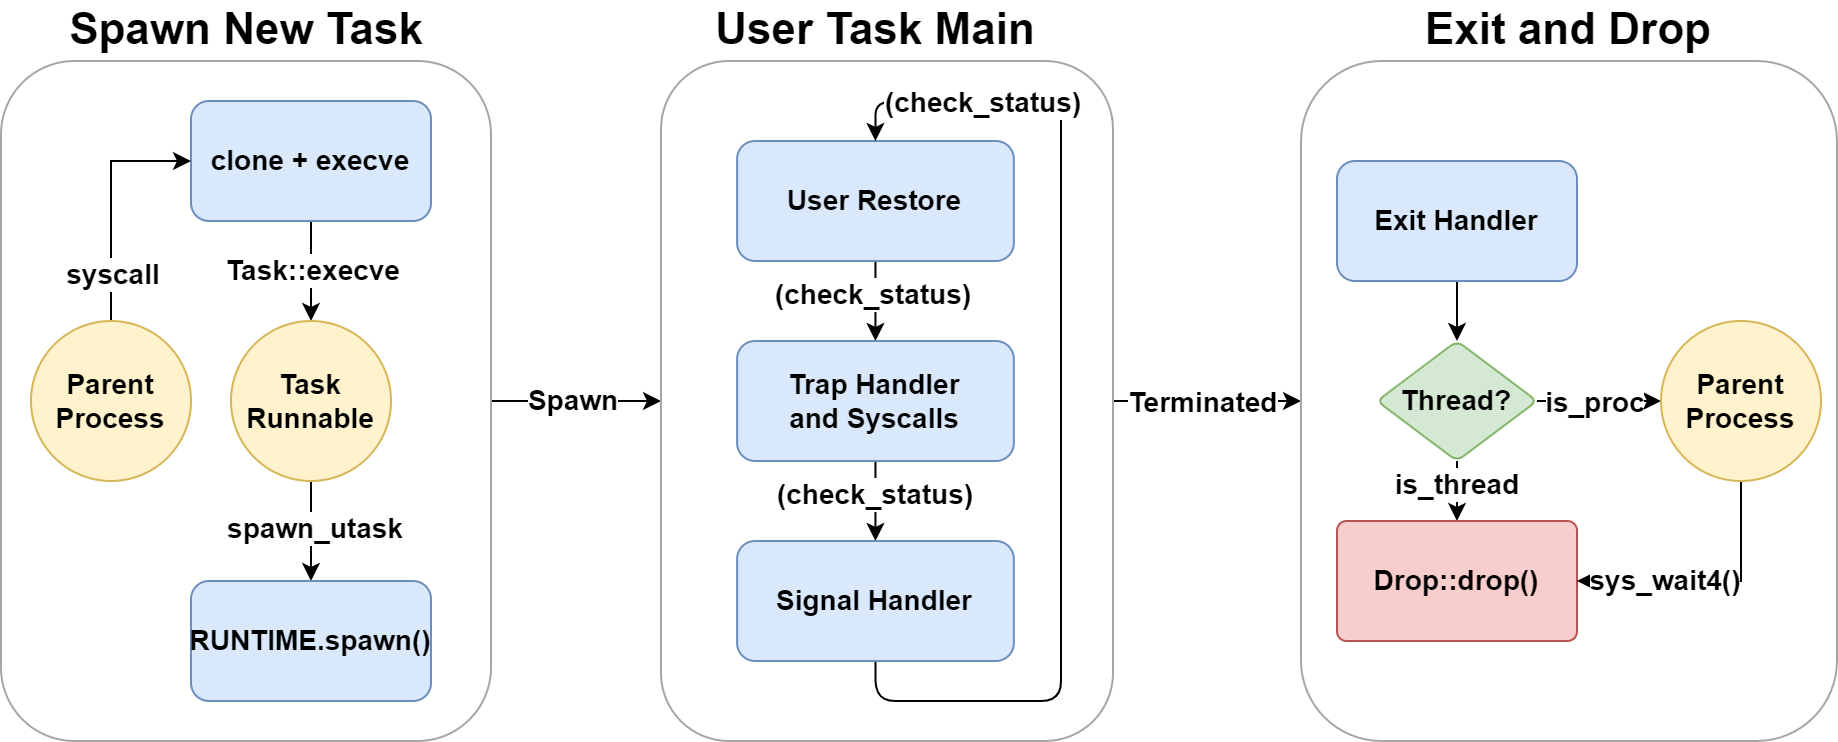
\includegraphics[width=1\linewidth]{assets//task/task_lifetime.drawio.png}
    \caption{任务生命周期}
    \label{fig:task_lifetime}
\end{figure}

\subsection{任务的创建}

\subsubsection{初始进程的加载}

在NoAxiom当中,初始进程以内嵌的二进制形式\code{.incbin}随内核一同加载到内存当中。在编译内核时,我们会提前编译好初始进程所需的elf文件,并通过\code{build.rs}构建到内核代码的\code{link_apps.S}。

例如,当选择的初始进程名为\code{run_busybox}时,我们生成的部分汇编代码如下:

\begin{lstlisting}
    .section .data
    .global run_busybox_start
    .global run_busybox_end
    .align 3
run_busybox_start:
    .incbin "../NoAxiom-OS-User/bin/run_busybox"
run_busybox_end:
\end{lstlisting}

在内核当中,我们通过自定义宏\code{use_apps!}通过编译选项自动选择初始进程名,并将对应的程序段链接到内核的可执行文件内。通过这种方式,NoAxiom可以快速修改用户程序的功能实现,并快速切换到所需的初始进程。

\begin{lstlisting}
macro_rules! use_app {
    ($name:literal) => {
        extern "C" {
            #[link_name = concat!($name, "_start")]
            fn app_start();
            #[link_name = concat!($name, "_end")]
            fn app_end();
        }
        pub const INIT_PROC_NAME: &str = $name;
    };
}
#[cfg(feature = "busybox")]
use_app!("run_busybox");
#[cfg(feature = "runtests")]
use_app!("run_tests");
\end{lstlisting}

由于初始进程的数据一开始位于内核数据段而不是文件系统当中,为了方便文件系统对于块设备的统一管理,复用从文件加载elf的代码,我们选择先通过\code{File::write_at}方法将内嵌的数据写入文件系统中,再通过创建的初始进程路径进行数据加载。

\begin{lstlisting}
pub fn schedule_spawn_with_path() {
    spawn_ktask(async move {
        let path_str = format!("/{}", INIT_PROC_NAME);
        let path = Path::from_or_create(path_str, InodeMode::FILE).await;
        let file = path.dentry().open().unwrap();
        file.write_at(0, get_file()).await.unwrap();
        let elf_file = path.dentry().open().unwrap();
        let elf = MemorySet::load_elf(&elf_file).await.unwrap();
        let task = Task::new_process(elf).await;
        spawn_utask(task);
    });
}
\end{lstlisting}

\subsubsection{普通任务的加载}

除了初始进程外的所有其他进程均依赖于\code{clone(2)}、\code{execve(2)}等系统调用来创建新任务。当执行\code{execve(2)}时,任务应当将当前执行的可执行文件镜像替换为另一文件镜像,初始化用户栈信息,更新用户上下文,关闭相应的任务资源,并终止其他线程运行。

\begin{lstlisting}
pub async fn execve(
    self: &Arc<Self>,
    path: Path,
    args: Vec<String>,
    envs: Vec<String>,
) -> SysResult<()> {
    let elf_file = path.dentry().open()?;
    let ElfMemoryInfo {
        memory_set,
        entry_point,
        user_sp,
        mut auxs,
    } = MemorySet::load_elf(&elf_file).await?;
    memory_set.memory_activate();
    self.terminate_threads();
    self.change_memory_set(memory_set);
    let (user_sp, _argc, _argv_base, _envp_base) =
        self.init_user_stack(user_sp, args, envs, &mut auxs);
    *self.trap_context_mut() = TrapContext::app_init_cx(entry_point, user_sp);
    self.sa_list().reset();
    self.fd_table().close_on_exec();
    Ok(())
}
\end{lstlisting}

\subsection{任务运行流程}

任务的运行是任务生命周期中占比最大的部分,任务将在用户态和内核态之间持续切换,并根据用户态异常的种类,提供系统调用服务或其他异常处理功能。任务的主要执行流程如\autoref{fig:task_main}所示。我们通过调用\code{UserTaskFuture}内部包装的异步函数来实现用户程序的执行。

\begin{figure}[H]
    \centering
    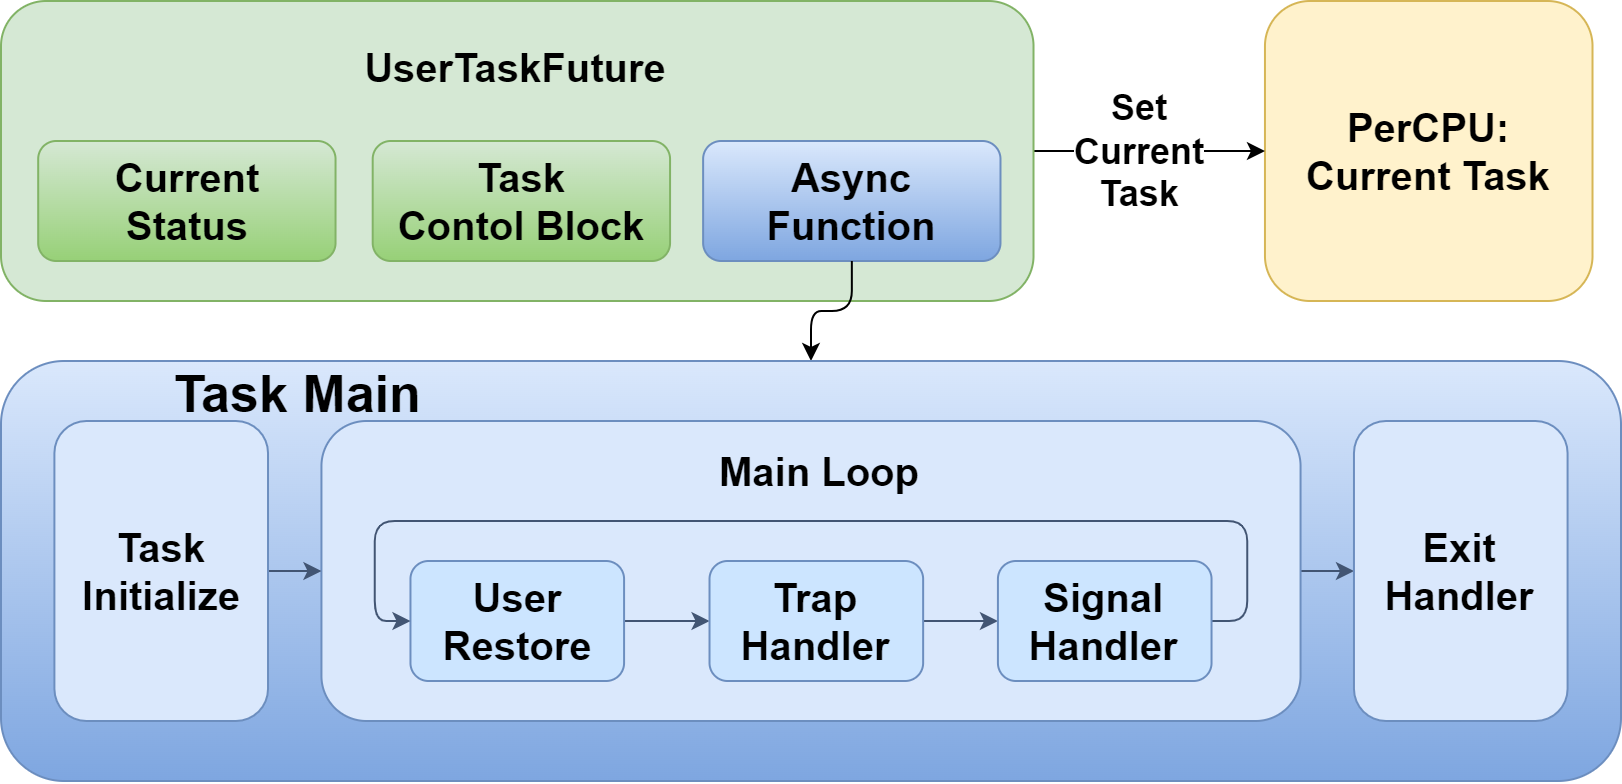
\includegraphics[width=0.75\linewidth]{assets//task/task_main.drawio.png}
    \caption{任务执行流程}
    \label{fig:task_main}
\end{figure}

\subsubsection{任务切换}

NoAxiom的所有任务均运行在异步运行时下,所有用户任务均被包装在异步的\code{UserTaskFuture}当中,等待执行器执行。在用户进程的生命周期内,其所有执行功能均在\code{UserTaskFuture}内部完成。

\code{UserTaskFuture}负责任务切换流程,当切入任务时,\code{UserTaskFuture}将会执行以下步骤:

\begin{enumerate}
    \item 关闭中断,保证任务切入的原子性。
    \item 记录当前任务的切入时间,便于进行时间统计和时间片维护。
    \item 访问当前核心的\code{per_cpu}字段,设置当前运行的任务控制块。
    \item 激活任务的地址空间,刷新TLB内缓存的地址翻译信息。
    \item 恢复任务在切出前记录的中断使能信息。
\end{enumerate}

而在切出任务时,\code{UserTaskFuture}也将镜像地执行上述行为,从而实现了任务信息切入切出的原子性与完整性。

\begin{lstlisting}
pub struct UserTaskFuture<F: Future + Send + 'static> {
    pub task: Arc<Task>,
    pub future: F,
}
impl<F: Future + Send + 'static> Future for UserTaskFuture<F> {
    type Output = F::Output;
    fn poll(self: Pin<&mut Self>, cx: &mut Context<'_>) -> Poll<Self::Output> {
        Arch::disable_interrupt();
        let this = unsafe { self.get_unchecked_mut() };
        let task = &this.task;
        let future = &mut this.future;
        task.time_stat_mut().record_switch_in();
        current_cpu().set_task(task);
        fence(Ordering::AcqRel);
        task.restore_cx_int_en();
        // ===== before executing task future =====
        let ret = unsafe { Pin::new_unchecked(future).poll(cx) };
        // ===== after executing task future =====
        task.record_cx_int_en();
        Arch::disable_interrupt();
        task.time_stat_mut().record_switch_out();
        current_cpu().clear_task();
        fence(Ordering::AcqRel);
        Arch::enable_interrupt();
        ret
    }
}
\end{lstlisting}

\subsubsection{任务主函数}

上节中的\code{UserTaskFuture}只负责任务信息的切入与切出,而实际的用户程序执行则在其内部包装的异步函数\code{task_main}中发生。异步函数\code{task_main()}负责任务主函数运行、用户上下文切换、任务退出等关键流程的执行,是真正意义上用于用户程序运行的主函数。

为了便于通过控制块进行任务唤醒,在进入用户程序的执行循环前,\code{task_main}将通过\code{take_waker}获取当前异步函数唤醒器并注册在任务控制块中。

在初始化完任务控制信息后,\code{task_main}将进入用户程序主循环,用于持续的内核/用户态切换,并向用户提供系统调用等服务功能。具体而言,用户程序主循环的执行流程如下:

\begin{enumerate}
    \item 恢复用户态执行:通过调用硬件抽象层的\code{trap_restore()}函数,恢复用户的执行上下文。此外,在进入用户态和返回内核态的过程中,将统计用户态的执行时间信息。
    \item 处理用户态例外:通过调用硬件抽象层的\code{read_trap_type},获取用户态发生的例外类型,并进入例外处理例程进行处理。该处理例程将提供系统调用、懒分配、写时复制、外部中断处理、时间片让权等关键内核功能的服务。
    \item 信号处理:检查是否存在挂起的未处理信号,若存在,则执行信号处理例程。
\end{enumerate}

此外,在每个执行流程之间,内核都将对当前任务状态进行检查,如果检测到当前任务已经被标记为退出(\code{TaskStatus::Terminated}),则将立即退出用户程序的循环执行,并执行退出处理例程\code{exit_handler()}。如果检测到当前任务被信号标记为暂停(\code{TaskStatus::Stopped}),则将立即挂起当前进程。

\begin{lstlisting}
pub async fn task_main(task: Arc<Task>) {
    task.set_waker(take_waker().await);
    loop {
        // kernel -> user, restore context and return to user mode
        task.time_stat_mut().record_trap_in();
        let cx = task.trap_context_mut();
        Arch::trap_restore(cx);
        let trap_type = Arch::read_trap_type(Some(cx));
        task.time_stat_mut().record_trap_out();
        match task.pcb().status() {
            TaskStatus::Terminated => break,
            TaskStatus::Stopped => suspend_now().await,
            _ => {}
        }
        // user -> kernel, enter the handler
        user_trap_handler(&task, trap_type).await;
        match task.pcb().status() {
            TaskStatus::Terminated => break,
            TaskStatus::Stopped => suspend_now().await,
            _ => {}
        }
        // check signal before return to user
        task.check_signal(None).await;
        match task.pcb().status() {
            TaskStatus::Terminated => break,
            TaskStatus::Stopped => suspend_now().await,
            _ => {}
        }
    }
    task.exit_handler().await;
}
\end{lstlisting}

\subsection{任务资源释放}

当任务在\code{task_main}函数中检测到当前状态为\code{Terminated}之后,将跳出用户程序的执行过程并执行退出处理例程\code{exit_handler}。这一过程标志着任务生命周期进入尾声。

Rust语言对于对象的生命周期做出了严格的规定,当对象生命周期结束时,将自动调用其析构方法。我们使用RAII的思想,使用Rust原生的\code{Arc<T>}原子引用计数指针包装任务控制块对象\code{Task},这是一个线程安全的共享指针,其内部将使用原子计数器\code{AtomicUsize}维护当前指针被引用的次数。当\code{Arc}指针的引用计数归零时,表明其生命周期结束,将会自动调用\code{Task}的\code{Drop::drop()}函数以释放内部资源。

对于线程而言,其资源应当由自身释放。当执行完毕线程的退出处理例程之后,线程的任务控制块\code{Arc<Task>}的引用计数归零,自动执行其\code{Drop}方法释放内部所有的线程独占资源。

对于进程而言,为了防止资源提前释放导致的资源错误复用问题,其内部资源应当延迟回收,由父进程负责通过\code{wait4()}等系统调用进行子进程资源的回收。我们已经在程序控制块\code{pcb}内部保存了每个进程的子进程的强引用\code{children: Vec<Arc<Task>>},可以避免子进程因为引用计数归零导致的提前释放。在检测到子进程退出后,父进程会将子进程的强引用从\code{children}字段中删除,使其引用计数清零而自动触发任务控制块的\code{Drop}方法。

\begin{figure}[H]
    \centering
    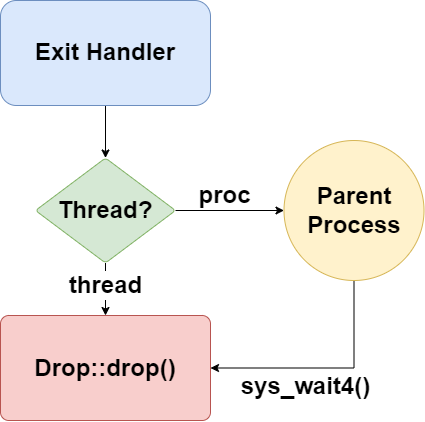
\includegraphics[width=0.5\linewidth]{assets//task/task_exit_handler.drawio.png}
    \caption{任务资源释放流程}
    \label{fig:task_exit_handler}
\end{figure}

\newpage
\section{内存管理}
\subsection{地址空间结构}
\subsubsection{内核地址空间初始化}

目前主流的地址空间设计大致分为共享地址空间和隔离地址空间两类。隔离的地址空间设计拥有更高的安全性,能够一定程度上防止侧信道攻击等针对缓存的攻击方式,但这种设计方式在切换用户/内核上下文时,需要频繁切换根页表并冲刷TLB,导致上下文切换的性能下降。

考虑到系统性能需求,NoAxiom选择将用户与内核共享地址空间,这种维护方式无需频繁切换根页表,有效避免了TLB冲刷开销。同时,为了在同一地址空间下隔离用户与内核空间,我们参照了Linux中的设计,选择将用户地址设置在低半地址空间,内核地址设置在高半地址空间。

具体而言,我们在硬件抽象层中根据具体架构定义了\code{KERNEL_ADDR_OFFSET}用于指示具体的高半地址空间前缀。这一前缀在RISC-V64架构中为\code{0xffff_ffc0_0000_0000},而这一前缀在LoongArch64架构中为\code{0x9000_0000_0000_0000}。

对于RISC-V64架构而言,RV64硬件级页表翻译使得我们能够便利地创建大页,因此NoAxiom将在系统启动时使用大页维护的临时页表进行启动维护,其内部将整个内核区域不区分读写权限地映射到了高半地址空间。在随后的初始化过程中,再创建内核对应的地址空间\code{KERNEL_SPACE: MemorySet},将具体的内核程序段映射到\code{0xffff_ffc0}开头的高半地址空间后,再激活真正的内核地址空间。

RV64中,在系统一开始启动时将会把页表设置给定的临时页表,并启动页表翻译功能。

\begin{lstlisting}
la      t0, {page_table}
srli    t0, t0, 12
li      t1, 8 << 60
or      t0, t0, t1
csrw    satp, t0
sfence.vma
\end{lstlisting}

对于LoongArch64架构而言,由于LA64架构支持了地址映射窗口,NoAxiom选择直接配置CSR寄存器中\code{DMWIN1}寄存器,将其地址映射窗口置为\code{0x9000}。由于在LoongArch架构中,在TLB进行地址翻译时,将会优先使用命中地址映射窗口的物理地址,因此也无需额外进行内核空间的页表初始化。

\begin{lstlisting}
ori         $t0, $zero, 0x11    # CSR_DMW1_MAT | CSR_DMW1_PLV0
lu52i.d     $t0, $t0, -1792     # CA, PLV0, 0x9000 xxxx xxxx xxxx
csrwr       $t0, 0x181          # LOONGARCH_CSR_DMWIN1
\end{lstlisting}

关于高半地址空间在系统启动时的具体维护事项,详见\ref{sec:hardware_bootstrap}中的描述。

\subsubsection{内核地址空间排布}

内核地址空间的排布较为简单,其地址空间按照内核可执行文件给定的程序段,从起始地址开始依次排布。而剩余的地址空间则用于进行物理页帧的分配。

\begin{itemize}
    \item 在LA64中,我们给定\code{ekernel}用于表示内核elf的结束地址。从起始地址到\code{ekernel}的数据均位于内核elf中,我们将通过内核elf给定的读写属性进行数据映射。
    \item 内核的\code{bss}段中将有部分空间用于维护内核堆空间,目前QEMU中的内核堆空间大小为48MB。
    \item 从\code{ekernel}开始一直到物理地址结束的空间将全部用于物理页帧分配,在现在的NoAxiom中,大约能够支持分配19000到20000个物理页帧。
    \item 为了避免用户更改内核内容,内核空间完全不支持用户态访问,我们选择将内核中的跳板页映射在用户空间中。
\end{itemize}

\subsubsection{用户地址空间排布}

由于启用了页表翻译功能,我们的用户地址空间可以较为宽松地进行配置,为不同类型的用户空间分配充足的虚地址空间。具体而言,以RISC-V64架构为例,我们的用户空间映射策略如 \autoref{table:user_address_space_ranges} 所示,其中按照地址从低到高以此给出了所有地址映射基址,映射长度及其对应的功能。

\begin{table}[h!]
\centering
\caption{用户空间映射区域表}
\label{table:user_address_space_ranges}
\begin{tabular}{l l l l}\toprule
    \textbf{功能}& \textbf{映射基址}& \textbf{(最大)映射长度}& 默认映射属性\\\midrule
    用户程序elf& 由用户程序决定& 由用户程序决定& 由用户程序决定\\
    用户栈stack& \code{ELF_END + 0x1000}& \code{0x80_0000}& R, W\\
    用户堆brk& \code{STACK_END + 0x1000}& \code{0x753_0000}& R, W\\
    共享内存shm& \code{0x5_0000_0000}& 由系统调用决定& 由系统调用给定\\
    内存映射mmap& \code{0x6_0000_0000}& \code{0x1000_0000}& 由系统调用给定\\
    信号跳板页& \code{0x1F_FFFF_F000}& \code{0x1000}& R, X\\\bottomrule
\end{tabular}
\end{table}

这里需要特别注意,与部分往届基于RISC-V架构的操作系统不同,NoAxiom选择将mmap区域的基址设置为更高的\code{0x6_0000_0000},以防止在LoongArch架构下与用户elf程序段起始地址\code{0x1_2000_0000}发生重叠而导致地址映射错误。

此外,我们专门在位于\code{USER_MEMORY_END - PAGE_SIZE},即用户映射区域尾段的位置映射了信号跳板页,专门用于执行内核提供的信号处理相关系统调用及其相关上下文切换操作,如\code{sigreturn}系统调用等,该页面由内核固定映射,每次加载内存区域时都会进行映射和相关指令的加载。

\subsection{内存管理器}
\subsubsection{堆分配管理器}

\code{no_std}环境下的Rust要求应当给定一个全局堆分配器用于进行堆空间申请。我们使用开源外部依赖库\code{buddy_system_allocator}作为NoAxiom的全局堆分配器,该依赖库使用伙伴算法对堆内数据进行维护。同时为了保证堆分配的原子性,我们使用关中断的\code{SpinLock}保护堆分配的过程。

此外,在NoAxiom当中,我们在\code{.bss}程序段预留了大小为48MB的堆空间用于堆分配器的初始化。当系统初始化的时候,将会对于堆空间调用\code{init}方法进行初始化。

\begin{lstlisting}
#[global_allocator]
static HEAP_ALLOCATOR: HeapAllocator = HeapAllocator::empty();
struct HeapAllocator(SpinLock<Heap<32>>);
unsafe impl GlobalAlloc for HeapAllocator {
    unsafe fn alloc(&self, layout: Layout) -> *mut u8 {
        self.0.lock().alloc(layout)
            .ok().map_or(0 as *mut u8, |allocation| allocation.as_ptr())
    }
    unsafe fn dealloc(&self, ptr: *mut u8, layout: Layout) {
        self.0.lock().dealloc(NonNull::new_unchecked(ptr), layout)
    }
}
\end{lstlisting}

\subsubsection{物理页帧管理器}

$\blacktriangleright$\textbf{接口抽象}

在NoAxiom中,我们将除了内核elf映射区域以外的所有区域均作为物理页帧空间进行管理。物理页帧(Physical Frame)固定分配大小为4KB,分配时将附带对应物理地址区域的初始化,并支持对于统一物理页帧进行引用计数。物理页帧参与了程序加载、页表分配、IO缓冲区等多种功能实现,是NoAxiom内核中最重要的内存分配方式之一。

\begin{lstlisting}
trait FrameAllocator {
    fn new() -> Self;
    fn alloc(&mut self) -> Option<PhysPageNum>;
    fn dealloc(&mut self, ppn: PhysPageNum);
}
\end{lstlisting}

$\blacktriangleright$\textbf{具体定义}

页帧分配器中维护了一个可变的页帧范围,其中\code{current}代表当前分配到的页帧号,\code{start}和\code{end}分别表示页帧区间的起始页号与终止页号。此外还有\code{recycled}数组维护空闲页帧,\code{frame_map}用于维护页帧计数映射。对于其具体的\code{alloc}和\code{dealloc},我们使用简易的栈式分配策略,将空闲的物理页帧插入到\code{Vec}当中进行维护。

\begin{lstlisting}
pub struct StackFrameAllocator {
    start: usize,
    current: usize,
    end: usize,
    recycled: Vec<usize>,
    frame_map: BTreeMap<usize, Weak<FrameTrackerInner>>,
}
impl FrameAllocator for StackFrameAllocator {
    fn alloc(&mut self) -> Option<PhysPageNum> {
        if let Some(ppn) = self.recycled.pop() {
            Some(ppn.into())
        } else if self.current == self.end {
            None
        } else {
            self.current += 1;
            Some((self.current - 1).into())
        }
    }
    fn dealloc(&mut self, ppn: PhysPageNum) {
        self.recycled.push(ppn.0);
    }
}
\end{lstlisting}

$\blacktriangleright$\textbf{引用计数}

为了便于进行写时复制的维护,我们对物理页帧使用\code{frame_map: BTreeMap}进行引用计数维护,其内部保存了物理页帧号到具体的物理页帧追踪器的映射,使用\code{Arc}相关的\code{strong_count()}进行引用计数查询,能够便利地查询当前物理页的引用情况。

\begin{lstlisting}
pub fn frame_refcount(ppn: PhysPageNum) -> usize {
    FRAME_ALLOCATOR
        .lock()
        .frame_map
        .get(&ppn.0)
        .map_or(0, |x| x.strong_count())
}
\end{lstlisting}

\subsubsection{资源占用维护}

$\blacktriangleright$\textbf{物理页帧分配限制}

在进行Unixbench的SHELL16测试点时,我们注意到即使是在qemu下运行系统,也容易因为大量申请进程空间而导致物理页帧不足,引发系统崩溃。为了防止这一情况发生,我们尝试在进行大批量的资源分配前进行内存空间的预先检查。例如,我们在进行elf文件映射前,会预先查看映射所需空间大小,如果发现映射后系统资源紧张则不予执行。

\begin{lstlisting}
pub fn can_alloc(&self, req_num: usize) -> bool {
    self.stat_remain() >= req_num
}
pub fn can_alloc_loosely(&self, req_num: usize) -> bool {
    // reserve 20% more frames for later use
    self.can_alloc(req_num + req_num / 5 + self.stat_total() / 20)
}
pub async fn map_elf(...) {
    if !can_frame_alloc_loosely(frame_req_num) {
        return_errno!(Errno::ENOMEM, "no enough frames to load elf");
    }
}
\end{lstlisting}

\subsection{地址空间维护}

在NoAxiom中,地址空间被定义为\code{MemorySet}对象保存在任务控制块中,并受到共享自旋锁保护。\code{MemorySet}的原始定义如下所示:

\begin{lstlisting}
pub struct MemorySet {
    pub page_table: SyncUnsafeCell<PageTable>,
    pub areas: Vec<MapArea>,
    pub stack: MapArea,
    pub brk: BrkAreaInfo,
    pub mmap_manager: MmapManager,
    pub shm: ShmInfo,
}
\end{lstlisting}

通过对于\code{MemorySet}进行访问,我们可以进行内存映射mmap维护、程序间断点brk维护、共享内存shm维护。在NoAxiom中,我们使用自旋锁\code{Arc<SpinLock<MemorySet>>}来保证地址空间信息维护的一致性。

% TODO!!!

\subsection{延迟分配技术}

\subsubsection{写时复制}

在以\code{clone(2)}为代表的进程复制操作过程当中,假如调用时未设置\code{VM_CLONE}标志位,则进程在创建新的子进程时需要将原有的内存信息完整地拷贝一份。通常这一行为将耗费大量的内存空间,为我们的内核带来极大的内存开销负担。

为了尽量避免进程复制时的内存复制开销,我们在内核中引入了写时复制(copy-on-write,COW)技术。具体而言,我们在物理页的页表项标志位(Page Table Entry Flags,PTEFlags)中,额外维护了一个特殊的扩展标记位COW用于标记某一页面正处于写时复制状态,并取消了对应页面的写标记位(Write Flag)用于捕获对应的用户态写入操作。当一个页面被标记为COW时,表示其应当复制,但当前仍由多个进程的地址空间共享。当该页面上发生用户写操作的时候,由于未设置W位,该写入操作将被操作系统捕获,并进行实际的页面复制行为。

$\blacktriangleright$\textbf{标记位定义}

我们在RV64和LA64的\code{PTEFlags}中均根据实际情况定义了该标记位\code{COW},并在上层的\code{MappingFlags}中创建了对应的虚拟标记位\code{COW},用于上层内核进行访问。

\begin{lstlisting}
pub struct MappingFlags: u64 {
    const COW = bit!(8);
}
/// RV64 PTE
pub struct PTEFlags: u64 {
    const COW = bit!(8);
}
/// LA64 PTE
pub struct PTEFlags: usize {
    const COW = bit!(9);
}
\end{lstlisting}

而在内核当中,我们会通过调用\code{flags_switch_to_cow}等函数,实现COW页面与普通页面的互转。

此外,值得一提的是,在LA64中W位的判断方式与其他常规架构存在较大差别。LA64中,TLB内部并不存储对应的W位,也不会进行相应的合法性检查。因此,假如直接置空W位并标记位COW,硬件仍然会正常地访问该页面而不会触发任何异常。因此在维护LA64架构下的COW行为时,我们选择了使用置空V位的方式来实现页表访问的异常捕获。

\begin{lstlisting}
#[inline(always)]
pub fn flags_switch_to_cow(flags: &MappingFlags) -> MappingFlags {
    *flags | MappingFlags::NV | MappingFlags::COW
}
#[inline(always)]
pub fn flags_switch_to_rw(flags: &MappingFlags) -> MappingFlags {
    *flags & !MappingFlags::NV | MappingFlags::V | MappingFlags::W
}
\end{lstlisting}

$\blacktriangleright$\textbf{延迟分配}

当用户或内核态访问某一携带\code{COW}标记的页面时,我们将通过各种方式检测到该标记,并通过\code{validate}函数调用\code{realloc_cow(vpn, pte)},最终实现某一页面的写时复制分配行为。

在实际分配的时候,我们还会对于页面的引用计数进行检查。当发现某一页面的引用计数为1时,说明该页面仅由当前线程独享,那么也就没有必要进行写时复制的再次分配了。我们只会将当前页面重置为正常页面,而不会进行额外页面的申请。

\begin{lstlisting}
pub fn realloc_cow(&mut self, vpn: VirtPageNum, pte: &PageTableEntry) -> SysResult<()> {
    let old_ppn = PhysPageNum::from(pte.ppn());
    let old_flags = pte.flags();
    let new_flags = flags_switch_to_rw(&old_flags);
    if frame_refcount(old_ppn) == 1 {
        self.page_table().set_flags(vpn, new_flags);
    } else {
        let frame = frame_alloc().unwrap();
        let new_ppn = frame.ppn();
        let mut target = None;
        // ... iterate memory_set and find the target
        self.page_table()
            .remap_cow(vpn, new_ppn, old_ppn, new_flags);
    }
    Arch::tlb_flush();
    Ok(())
}
\end{lstlisting}

\subsubsection{懒分配}

我们在内存映射(mmap)、程序间断点(brk)、 用户栈(stack)的分配过程中使用了懒分配技术。具体而言,在用户程序申请对应资源的时候,我们并不会在实际页表上进行页面信息的映射,而是将对应页面保存到当前\code{MemorySet}中。当用户读取对应页面的数据,会因为页面未映射而触发缺页异常,从而使得访存行为被内存捕获。此时再进行真正的分配过程。

\subsubsection{合法性检查与分配}

我们使用\code{validate()}函数对于某个具体的访存相关异常进行验证,假如检测到位于写时复制或者懒分配区域,则访问地址空间并对于具体的区域进行分配操作。

\begin{itemize}
    \item 写时复制:我们会首先检查当前发生缺页异常的页面是否真实存在,如果检测到页面存在,则说明该页面可能是一个被标记为COW的页面。紧接着检查当前页面的COW标志位,假如的确存在,则进行写时复制处理,否则报出地址错误,由对应系统调用或者例外处理例程进行响应。
    \item 懒分配:假如检测到页面不存在,则说明该页面可能是一个懒分配页面。我们将依次访问内存空间当中维护的stack、brk、mmap区域,检查是否的确存在一个对应的页面尚未分配。若未分配,则进行懒分配操作,否则报出地址错误,由对应系统调用或者例外处理例程进行响应。
\end{itemize}

\begin{lstlisting}
pub async fn validate(
    memory_set: &Arc<SpinLock<MemorySet>>,
    vpn: VirtPageNum,
    trap_type: Option<TrapType>,
    pte: Option<&mut PageTableEntry>,
) -> SysResult<()> {
    if let Some(pte) = pte {
        let flags = pte.flags();
        if flags.contains(MappingFlags::COW) {
            memory_set.lock().realloc_cow(vpn, pte)?; // copy-on-write allocation
            Ok(())
        } else {
            Err(Errno::EFAULT)
        }
    } else {
        let mut ms = memory_set.lock();
        if ms.stack.vpn_range.is_in_range(vpn) {
            let task = current_task().unwrap();
            ms.lazy_alloc_stack(vpn); // stack lazy allocation
            Ok(())
        } else if ms.brk.area.vpn_range.is_in_range(vpn) {
            ms.lazy_alloc_brk(vpn); // brk(heap) lazy allocation
            Ok(())
        } else if ms.mmap_manager.is_in_space(vpn) {
            drop(ms);
            lazy_alloc_mmap(memory_set, vpn).await?; // mmap lazy allocation
            Ok(())
        } else {
            Err(Errno::EFAULT)
        }
    }
}
\end{lstlisting}

\subsection{用户指针}

在大量系统调用中都涉及用户态传入指针及其合法性检查的步骤。为了规范化用户态指针验证步骤,我们设计了用户指针\code{UserPtr}专门用于进行用户地址空间指针的访问。其本体只包装了一个裸指针地址,其安全性由访问时的合法性检查保证。

\begin{lstlisting}
pub struct UserPtr<T = u8> {
    _phantom: PhantomData<T>,
    addr: usize,
}
\end{lstlisting}

\subsubsection{基于异常的指针预检查}\label{sec:user-ptr-check}

在验证用户指针合法性时,我们参考了优秀开源项目Phoenix\footnote{https://gitlab.eduxiji.net/educg-group-22026-2376550/T202418123993075-1053}的实现思路,设计了适用于NoAxiom的指针验证方式。在进行用户指针检查时,arch层将通过临时替换异常入口并尝试进行一个字节的读写操作来验证页面的合法性。该设计有效利用了当前TLB内缓存的页表映射信息,避免了直接访存导致的cache miss,有效提升了验证时性能。

由于这一实现与具体架构中异常替换以及异常种类转化相关,我们将具体的指针验证过程放置在了arch层,而内核当中则通过\code{Arch::check_read(addr)}和\code{Arch::check_write(addr)}进行指针合法性检查,这两个函数会对于对应地址的读写属性进行检查,若检测出页面异常则会通过\code{Err(TrapType)}返回异常类型。

\begin{lstlisting}
pub type UserPtrResult = Result<(), TrapType>;
pub trait ArchTrap {
    fn check_read(addr: usize) -> UserPtrResult;
    fn check_write(addr: usize) -> UserPtrResult;
}
\end{lstlisting}

就架构而言,以RV64架构为例,其具体处理\code{check_read}的过程如下,对于读取操作,内核尝试读取一字节的数据,并有可能在这个过程中触发异常。这里需要注意,应当提前关闭RV64的压缩指令优化,以防止后续通过\code{epc}自增跳过指令时出现错误的指令对齐地址情况。

\begin{lstlisting}
unsafe fn bare_read(ptr: usize) {
    asm!(
        ".option push
        .option norvc
        lb a0, 0(a0) # exception happens here
        .option pop",
        in("a0") ptr,
    );
}
\end{lstlisting}

为了方便实现,我们在全局设置了per-cpu的\code{USER_PTR_TRAP_TYPE},在访问用户指针之前将其设置为\code{None},假如访问后检测到其数值发生了变化,则说明访问过程中发生了异常。

\begin{lstlisting}
/// NoAxiom/lib/arch/src/rv64/trap.rs
#[repr(align(64))]
#[derive(Copy, Clone, Debug, PartialEq, Eq)]
struct Wrapper(TrapType);
static mut USER_PTR_TRAP_TYPE: [Wrapper; CPU_NUM] = [Wrapper(TrapType::None); CPU_NUM];
unsafe fn before_user_ptr() {
    RV64::disable_interrupt();
    set_ptr_entry();
    // clear trap_type for trap handler
    USER_PTR_TRAP_TYPE[RV64::get_hartid()] = Wrapper(TrapType::None);
}
unsafe fn after_user_ptr() -> UserPtrResult {
    // reload trap_type to check the validality
    let trap_type = volatile_load(&USER_PTR_TRAP_TYPE[RV64::get_hartid()]).0;
    let res = match trap_type {
        TrapType::None => Ok(()),
        _ => Err(trap_type),
    };
    set_kernel_trap_entry();
    RV64::enable_interrupt();
    res
}
\end{lstlisting}

当发生异常时,内核会首先跳转到预先设置的异常处理入口\code{__kernel_user_ptr_vec}处理函数中,紧接着将对应的\code{USER_PTR_TRAP_TYPE}设置为从\code{scause}中读取的内容,最后返回主控制流,由主控制流再进行访存,并检测异常类型。

\begin{lstlisting}
pub unsafe extern "C" fn kernel_user_ptr_handler() {
    let hartid = RV64::get_hartid();
    let scause = scause::read();
    let stval = stval::read();
    let sepc = sepc::read();
    sepc::write(sepc + 4); // skip read
    USER_PTR_TRAP_TYPE[hartid] = Wrapper(get_trap_type(scause, stval));
}
unsafe fn check_read(ptr: usize) -> UserPtrResult {
    before_user_ptr();
    bare_read(ptr);
    after_user_ptr()
}
/// NoAxiom/lib/arch/src/rv64/trap.S
__kernel_user_ptr_vec:
KERNEL_SAVE_REG
call      kernel_user_ptr_handler
KERNEL_LOAD_REG
sret
\end{lstlisting}

\subsubsection{用户指针的延迟分配与异步读取}

我们认为检测出用户态指针异常是一件小概率事件,因此在异常发生后的延迟分配过程中,我们无需过度关注性能表现。根据异常的类型不同,我们会访问内存空间并依次对于写时复制、堆栈空间、mmap空间等进行合法性验证。一旦检测到存在延迟分配行为,则真正进行资源分配。这一逻辑在\code{validate()}函数当中实现。

NoAxiom系统最大的特点是尽可能追求一切操作的完全异步,在无栈协程架构内尽可能避免让权行为的发生。对于用户指针的懒分配过程,我们也做到了这一点。

由于懒分配中可能存在文件读取行为,该分配过程是有概率进行让权的。我们观察到往年的作品在文件懒分配里的处理都是直接使用阻塞逻辑进行读取,这造成了性能的大量损失。而我们通过将用户指针验证包装为异步函数的方式,实现了用户指针的\textbf{异步读取让权}行为。

具体而言,我们以对单个地址的读取为例,详细解释某个指针的合法性验证过程。

当尝试对某一地址进行读取时,首先我们会对于指针的合法性进行检查。这主要包含了两方面:指针是否为空,以及指针对应的物理页是否合法。

对于指针对应页面合法性的检查,我们使用了上一节\ref{sec:user-ptr-check}中的检查方式,使用\code{check_read(addr)}进行某一单一指针的合法性检查。

此外,当我们检测到当前验证函数执行于某一自旋锁内部的时候,为了防止进程切出导致的死锁,我们选择进行阻塞式的内存验证行为。

\begin{lstlisting}
pub async fn read(&self) -> SysResult<T>
where
    T: Copy,
{
    if self.is_null() {
        return Err(Errno::EFAULT);
    }
    match Arch::check_read(self.addr()) {
        Ok(()) => Ok(unsafe { self.read_unchecked() }),
        Err(trap_type) => match trap_type {
            TrapType::LoadPageFault(addr) | TrapType::StorePageFault(addr) => {
                let task = current_task().unwrap();
                if check_no_lock() {
                    task.memory_validate(addr, Some(trap_type), false).await?;
                } else {
                    block_on(task.memory_validate(addr, Some(trap_type), true))?;
                }
                Ok(unsafe { self.read_unchecked() })
            }
            _ => return Err(Errno::EFAULT),
        },
    }
}
\end{lstlisting}

例如,当内核试图从用户空间中读取时,将会调用\code{ptr.read().await?},保证用户空间的正确性。其中使用了Rust的\code{?}关键字用于简便返回\code{Result}类型返回值中\code{Err(_)}的情况。

\begin{lstlisting}
// sys_setitimer
let new_value = UserPtr::<ITimerVal>::new(new_value);
let new_value = new_value.read().await?;
\end{lstlisting}

\newpage
\section{硬件抽象层}
\subsection{双架构支持概览}

由于NoAxiom的内核架构是从零自主研发的,为了适配赛事的双架构环境,我们设计了独属于NoAxiom操作系统内核的硬件抽象层NoAxiom-Arch,通过\code{Arch}对象抽象实现了内核与硬件的完全解耦。

目前,NoAxiom的硬件抽象层支持从RISCV64、LoongArch64双架构,支持双架构下从qemu启动,支持双架构统一内存管理、TLB管理,支持双架构统一中断异常处理过程,此外还支持时钟维护等其他架构相关的解耦维护。

NoAxiom-Arch向上仅暴露了\code{Arch}对象及其相关实现的若干\code{trait}属性。我们应用面向对象多态的设计思想,通过\code{trait}重载虚函数的方式,将硬件抽象接口统一为一致的接口,供给内核调用。

\subsection{硬件架构解耦设计}

NoAxiom中,所有涉及指令集架构的操作均被统一为\code{Arch}对象中的不同方法供kernel调用。编译时,我们将根据选择的架构不同,为\code{Arch}选定对应的底层实现。

\begin{lstlisting}
#[cfg(target_arch = "loongarch64")]
pub type Arch = la64::LA64;
#[cfg(target_arch = "riscv64")]
pub type Arch = rv64::RV64;
\end{lstlisting}

在NoAxiom-Arch中,硬件相关的不同功能被具体分类为中断使能控制、内嵌汇编、中断异常陷入处理、时间管理、系统启动、架构信息等子模块,这些子模块被包含在对应的特性\code{trait}当中,并由顶层特性\code{FullArch}统一管理。我们规定\code{Arch}应当实现\code{FullArch},并通过该特性向内核传递具体的方法调用。

\begin{lstlisting}
pub trait ArchFull:
    ArchInt + ArchAsm + ArchSbi + ArchTrap + ArchTime + ArchBoot + ArchInfo {}
pub struct LA64;
impl crate::ArchFull for LA64 {}
pub struct RV64;
impl crate::ArchFull for RV64 {}
\end{lstlisting}

\subsection{硬件初始化}\label{sec:hardware_bootstrap}

在NoAxiom中,硬件相关的初始化分为两部分:

\begin{enumerate}
    \item 系统从bootloader启动后刚进入内核代码时,HAL层通过\code{entry}汇编代码块,进行初始的内核相关控制寄存器配置。我们称之为\code{early_init}。
    \item 系统从HAL层进入到kernel层进行初始化后,在初始化过程中需要额外进行与硬件相关的初始化过程。我们称之为\code{kernel_arch_init}。
\end{enumerate}

\subsubsection{启动时初始化}

由于汇编代码要求程序给定\code{_entry},我们并没有为entry相关的函数配置对应的\code{trait}内函数,而是直接嵌入到代码中。

当程序从bootloader跳转到\code{_entry}进行初始化的时候,我们会进行启动时临时页表配置,这主要是为了适配我们内核的高低半地址空间的设计。除此之外,还会进行内核栈空间的配置,我们通过预留的内核栈空间指针,将不同核心绑定到对应的内核栈上。

对于两个架构而言,我们都会预先为每个核心预留一个内核栈,并在初始化的时候进行内核栈的设置。下文中的汇编代码片段展示了rv64中的内核栈初始化过程,该过程在la中基本一致。具体而言,在启动时,我们会获取当前核心的cpuid号,并通过该id号与单一内核栈大小相乘,以此获取对应的内核栈顶地址。

\begin{lstlisting}
#[link_section = ".bss.kstack"]
pub(crate) static BOOT_STACK: [u8; KERNEL_STACK_SIZE * CPU_NUM] = [0; KERNEL_STACK_SIZE * CPU_NUM];

asm!("
    add     t0, a0, 1
    slli    t0, t0, {kernel_stack_shift}
    la      sp, {boot_stack}
    add     sp, sp, t0
    li      s0, {kernel_addr_offset}
    or      sp, sp, s0
    li      t1, {kernel_addr_offset}
    or      gp, gp, t1
");
\end{lstlisting}

$\blacktriangleright$\textbf{RISC-V64临时页表初始化}

rv64中,由于分配了内核位于高半地址空间但内核空间并未分配,我们需要使用预先定义的初始化时页表来充当临时页表进行翻译。该页表会将\code{0xffff_fc00_8000_0000}开头的地址映射到低半空间的物理地址上,实现内核空间的正常访问。

\begin{lstlisting}
#[link_section = ".data.prepage"]
static PAGE_TABLE: [usize; PTE_PER_PAGE] = {
    let mut arr: [usize; PTE_PER_PAGE] = [0; PTE_PER_PAGE];
    macro_rules! page_table_config {
        ($($id:expr, $addr:expr)*) => {
            $(arr[$id] = ($addr << 10) | 0xcf;)*
        };
    }
    page_table_config! {
        2, 0x80000
        0x102, 0x80000
    };
    arr
};

// activate page table
asm!("
    la      t0, {page_table}
    srli    t0, t0, 12
    li      t1, 8 << 60
    or      t0, t0, t1
    csrw    satp, t0
    sfence.vma
");
\end{lstlisting}

$\blacktriangleright$\textbf{LoongArch64内存映射窗口配置}

在LA64中,我们为了便于维护,选择直接配置LA64下的内存映射窗口,将\code{0x8000}与\code{0x9000}开头的地址段标记为内核可访问,以此实现高地址空间的内存映射。

\begin{lstlisting}
asm!("
    ori         $t0, $zero, 0x1     # CSR_DMW1_PLV0
    lu52i.d     $t0, $t0, -2048     # UC, PLV0, 0x8000 xxxx xxxx xxxx
    csrwr       $t0, 0x180          # LOONGARCH_CSR_DMWIN0
    ori         $t0, $zero, 0x11    # CSR_DMW1_MAT | CSR_DMW1_PLV0
    lu52i.d     $t0, $t0, -1792     # CA, PLV0, 0x9000 xxxx xxxx xxxx
    csrwr       $t0, 0x181          # LOONGARCH_CSR_DMWIN1
")
\end{lstlisting}

$\blacktriangleright$\textbf{内核入口跳转}

在全部初始化完成之后,我们将会跳转到内核当中预留的真正入口\code{_boot_hart_init}中,退出汇编进行进一步的初始化过程。下面展示了rv64中相关的跳转操作。

\begin{lstlisting}
asm!("
    mv      a1, gp
    la      t0, {entry}
    or      t0, t0, t1
    mv      a0, tp
    jalr    t0
"),
entry = sym _boot_hart_init
\end{lstlisting}

\subsubsection{内核功能初始化}

在NoAxiom中,我们设计了\code{trait ArchBoot}用于进行系统初始化相关的内核调用接口,其内部搭载了\code{arch_init}函数用于进行初始化。

\begin{lstlisting}
pub trait ArchBoot {
    fn arch_init();
}
\end{lstlisting}

$\blacktriangleright$\textbf{LoongArch64}

对于la64而言,其初始化过程包含了浮点寄存器、异常中断向量入口、时钟模块、页表翻译(tlb)相关的初始化。其具体初始化过程不再赘述。

\begin{lstlisting}
impl ArchBoot for LA64 {
    fn arch_init() {
        freg_init();
        trap_init();
        time_init();
        tlb_init();
    }
}
\end{lstlisting}

$\blacktriangleright$\textbf{RISC-V64}

而对于rv64而言,由于页表翻译过程由硬件接管,我们在一开始启动的时候并不需要对于tlb相关寄存器进行特殊配置。此外,由于RISCV特有的SBI接口的存在,我们不需要特地配置时钟相关的初始化。只需要进行例外入口和浮点寄存器初始化即可。

\begin{lstlisting}
impl ArchBoot for RV64 {
    fn arch_init() {
        trap_init();
        freg_init();
    }
}
\end{lstlisting}

\subsection{页表管理}

\subsubsection{页表抽象}

在我们的\code{ArchMemory}中,对于页表抽象进行了给定。

\begin{lstlisting}
/// memory management arch trait
pub trait ArchMemory {
    const PHYS_MEMORY_START: usize;
    const PHYS_MEMORY_END: usize;
    const KERNEL_ADDR_OFFSET: usize;
    type PageTable: ArchPageTable;
    fn tlb_init();
    fn tlb_flush();
    fn current_root_ppn() -> usize;
    fn activate(ppn: usize, is_kernel: bool);
}
\end{lstlisting}

可以看到,我们设计了\code{ArchPageTable}特性,并定义了\code{type PageTable: ArchPageTable}用于向内核提供统一的页表定义接口,借此限定底层的具体实现。

而对于\code{ArchPageTable}的具体实现,我们进一步提供了\code{PageTableEntry}接口,用于限定单个页表项的访问行为。并提供了获取当前根页表页帧号、创建新页表、激活某一页表等一系列功能,向内核提供统一的访问接口。

\begin{lstlisting}
pub trait ArchPageTable {
    type PageTableEntry: ArchPageTableEntry;

    /// virtual address width
    const VA_WIDTH: usize;
    /// index level number
    const INDEX_LEVELS: usize;

    fn root_ppn(&self) -> usize;
    fn new(root_ppn: usize) -> Self;
    fn activate(&self);
}
\end{lstlisting}

\subsubsection{页表项抽象}

在RV64和LA64中,页表项的维护策略并不完全相同,根据我们对于硬件架构的了解,我们将页表项异同总结如下:

\begin{itemize}
    \item 相同点:均保持了物理页帧号+标记位的结构,且均具备RWV等基本的标记位。
    \item 不同点:物理页帧号保存的偏移不同,标记位的具体位置不同。
\end{itemize}

我们将相同点统合为\code{ArchPageTableEntry}这一类型,该类型通过\code{MappingFlags}向内核提供一个软件模拟的页表控制位,并在与硬件层交互时,将其转化为具体的对应PTE中的控制位。同时,由于PTE中的物理页帧号的维护需求基本相同,我们选择使用统一传入的物理页帧号,与\code{MappingFlags}拼接,最终形成对应硬件架构下的PTE值。

\begin{lstlisting}
pub trait ArchPageTableEntry: Into<usize> + From<usize> + Clone {
    /// create a new page table entry from ppn and flags
    fn new(ppn: usize, flags: MappingFlags) -> Self;
    /// get the physical page number
    fn ppn(&self) -> usize;
    /// get the pte permission flags
    fn flags(&self) -> MappingFlags;
    /// set flags
    fn set_flags(&mut self, flags: MappingFlags);
    /// clear all data
    fn reset(&mut self);
    /// is valid dir
    fn is_allocated(&self) -> bool;
}
\end{lstlisting}

这里需要强调,\code{ArchPageTableEntry}向内核暴露的接口中,传入的控制参数均为\code{MappingFlags}类型,但我们会在底层设置时,将该flag进一步转化为硬件定义的\code{PTEFlags}再进行设置。

我们对于虚拟页表项控制位\code{MappingFlags}的定义如下所示。可以看到,除了常规的\code{V, R, W, X}等标记位以外,我们定义了三个特殊的标记位\code{COW, NV, PT}。其中,\code{COW}位用于写时复制标记,\code{NV}用于强制标识当前页面不合法,\code{PT}用于强制标识当前页面为页表中的非叶节点,主要用于简化LA下的页表遍历过程。

\begin{lstlisting}
bitflags! {
    /// Mapping flags for page table.
    #[derive(Debug, Clone, Copy, PartialEq, Eq, PartialOrd, Ord, Hash)]
    pub struct MappingFlags: u64 {
        const V = bit!(0);
        const R = bit!(1);
        const W = bit!(2);
        const X = bit!(3);
        const U = bit!(4);
        const G = bit!(5);
        const A = bit!(6);
        const D = bit!(7);
        const COW = bit!(8);
        /// OS-specific: virt bit to specify the invalid page
        const NV = bit!(62);
        /// OS-specific: virt bit for page table
        const PT = bit!(63);
    }
}
\end{lstlisting}

$\blacktriangleright$\textbf{RV64页表项转化}

在RV64架构下,PTE中保存的控制位的真实定义如下,可以看到,与\code{MappingFlags}并不完全相同,我们还需要进一步的映射来实现真实控制位的设置。

\begin{lstlisting}
bitflags! {
    #[derive(Debug, Clone, Copy, PartialEq, Eq, PartialOrd, Ord, Hash)]
    pub struct PTEFlags: u64 {
        const V = bit!(0);
        const R = bit!(1);
        const W = bit!(2);
        const X = bit!(3);
        const U = bit!(4);
        const G = bit!(5);
        const A = bit!(6);
        const D = bit!(7);
        const COW = bit!(8);
    }
}
\end{lstlisting}

而在进行\code{MappingFlags}到\code{PTEFlags}的转化中,我们将实现对应控制位的一一映射行为。在下面的代码中,我们通过宏定义实现了RWXUGAD等控制位的转换。

\begin{lstlisting}
impl From<MappingFlags> for PTEFlags {
    fn from(flags: MappingFlags) -> Self {
        if flags.is_empty() {
            Self::empty()
        } else if flags.contains(MappingFlags::PT) {
            Self::V
        } else {
            let mut res = Self::empty();
            macro_rules! set {
                ($($flag:ident),*) => {
                    $(
                        if flags.contains(MappingFlags::$flag) {
                            res |= PTEFlags::$flag;
                        }
                    )*
                };
            }
            if flags.contains(MappingFlags::V) && !flags.contains(MappingFlags::NV) {
                res |= PTEFlags::V;
            }
            set!(R, W, X, U, G, A, D, COW);
            res
        }
    }
}
\end{lstlisting}

$\blacktriangleright$\textbf{LA64页表项转化}

LA64下的页表项与RV64类似,不过由于出现了更多未在\code{MappingFlags}中描述的控制位,我们对于未定义位使用了统一的映射方式进行控制。

这里值得一提的,为了优化LA下的TLB访问行为,我们选择将所有页表内非叶节点的项的flag置空,这样就可以避免TLB查询时对于控制位的额外计算了;但在RV中,中间项也必须设置V标记位,用于指示当前页表项的合法性。下面列出了RV和LA下对于\code{MappingFlags::PT}的不同处理。

\begin{lstlisting}
// RV64: set V flag
if flags.contains(MappingFlags::PT) {
    Self::V
}
// LA64: set empty, for TLB iteration pref
if flags.contains(MappingFlags::PT) {
    return PTEFlags::empty();
}
\end{lstlisting}

\subsubsection{TLB维护}

LA64与RV64下的TLB重填维护存在很大不同,其主要原因是LA64下的TLB重填过程由软件负责,而RV64下该行为则几乎完全依赖硬件实现。这导致LA64下需要额外地进行TLB重填相关操作的维护。

$\blacktriangleright$\textbf{TLB初始化}

具体而言,LA64下在系统初始化时,我们就会进行TLB重填的相关寄存器初始化。我们的内核的页面大小固定位4KB,因此会在初始化时向对应csr寄存器固定设置页面大小为\code{PS_4K}。除此之外,还会进行\code{pwcl}和\code{pwch}寄存器的配置,用于控制页表翻译过程中每级在虚地址中对应的数位范围。

最终当所有寄存器初始化完成后,我们会调用\code{set_tlb_refill_entry}设置TLB重填异常的入口,并冲刷TLB使能该设置。

\begin{lstlisting}
pub fn tlb_init_inner() {
    // Page Size 4KB
    const PS_4K: usize = 0x0c;
    tlbidx::set_ps(PS_4K);
    stlbps::set_ps(PS_4K);
    tlbrehi::set_ps(PS_4K);
    // Set Page table entry width
    pwcl::set_pte_width(8);
    // Set Page table width and offset
    pwcl::set_ptbase(12);
    pwcl::set_ptwidth(9);
    pwcl::set_dir1_base(21);
    pwcl::set_dir1_width(9);
    pwcl::set_dir2_base(30);
    pwcl::set_dir2_width(9);
    pwch::set_dir3_base(39);
    pwch::set_dir3_width(9);
    set_tlb_refill_entry(__tlb_refill as usize);
}
\end{lstlisting}

$\blacktriangleright$\textbf{TLB重填异常}

我们在\code{__tlb_refill}当中使用汇编嵌入了一段TLB重填的处理例程,在陷入TLB重填异常时,将会通过\code{tlbrentry}寄存器的值跳转到该函数对应的PC值,并进行TLB重填处理。重填过程将会遍历四级页表并将获取到的PTE填入TLB中。

\begin{lstlisting}
.globl    __tlb_refill
.balign   4096
__tlb_refill:
    csrwr     $t0, LA_CSR_TLBRSAVE
    csrrd     $t0, LA_CSR_PGD
    lddir     $t0, $t0, 3
    lddir     $t0, $t0, 2
    lddir     $t0, $t0, 1
    ldpte     $t0, 0
    ldpte     $t0, 1
    tlbfill
    csrrd     $t0, LA_CSR_TLBRSAVE
    ertn
\end{lstlisting}

\subsection{异常处理}

\subsubsection{异常处理抽象}

异常处理过程由于涉及到特定CSR寄存器的读写操作,因此也与硬件架构强耦合。我们选择使用\code{ArchTrap}特性实现异常处理的抽象接口。该接口包含了异常初始化\code{trap_init}、上下文切换\code{trap_restore}、异常状态读取\code{read_trap_type}等操作,同时对于用户指针合法性验证,使用\code{check_read}和\code{check_write}函数进行维护。

\begin{lstlisting}
pub trait ArchTrap {
    type TrapContext: ArchTrapContext;
    fn trap_init();
    fn trap_restore(_cx: &mut <Self as ArchTrap>::TrapContext);
    fn read_epc() -> usize;
    fn read_trap_type(cx: Option<&mut <Self as ArchTrap>::TrapContext>) -> TrapType;
    fn check_read(addr: usize) -> UserPtrResult;
    fn check_write(addr: usize) -> UserPtrResult;
}
\end{lstlisting}

\subsubsection{异常类型抽象}

由于不同架构下对于异常类型的定义不相同,我们设计了统一的抽象异常类型\code{TrapType}用于向内核提供统一的异常访问接口。定义如下所示,其中与访存相关的错误会额外包含一个\code{usize}表示的地址,用于指示导致异常的地址,用于内核验证内存时使用。

\begin{lstlisting}
pub enum TrapType {
    Breakpoint,
    SysCall,
    Timer,
    Unknown,
    SupervisorExternal,
    SupervisorSoft,
    StorePageFault(usize),
    LoadPageFault(usize),
    InstructionPageFault(usize),
    IllegalInstruction(usize),
    None,
}
\end{lstlisting}

\subsubsection{异常类型转化}

$\blacktriangleright$\textbf{RV64下的异常类型转化}

我们的异常类型主要基于RV64进行设计,因此RV64架构下的异常类型转化接近于直接映射的行为。具体而言,我们会预先读取RV64下用于指示异常的\code{scause}与\code{stval}的值,并将其传入\code{get_trap_type}中,由该函数进行进一步的映射。

\begin{lstlisting}
pub fn get_trap_type(scause: Scause, stval: usize) -> TrapType {
    match scause.cause() {
        Trap::Exception(Exception::LoadFault) => TrapType::Unknown,
        Trap::Exception(Exception::UserEnvCall) => TrapType::SysCall,
        Trap::Interrupt(Interrupt::SupervisorTimer) => TrapType::Timer,
        Trap::Exception(Exception::StorePageFault) => TrapType::StorePageFault(stval),
        Trap::Exception(Exception::StoreFault) => TrapType::StorePageFault(stval),
        Trap::Exception(Exception::InstructionPageFault) => TrapType::InstructionPageFault(stval),
        Trap::Exception(Exception::IllegalInstruction) => TrapType::IllegalInstruction(stval),
        Trap::Exception(Exception::LoadPageFault) => TrapType::LoadPageFault(stval),
        Trap::Interrupt(Interrupt::SupervisorExternal) => TrapType::SupervisorExternal,
        Trap::Interrupt(Interrupt::SupervisorSoft) => TrapType::SupervisorSoft,
        _ => panic!("unknown trap type: {:?}", scause.cause()),
    }
}
\end{lstlisting}

$\blacktriangleright$\textbf{LA64下的异常类型转化}

LA64下的异常类型转化相对较为复杂,由于LA64下定义了\code{AddressNotAligned}等需要特殊处理的异常类型,我们无法建立其与\code{TrapType}的直接映射,而是需要先进行合法性检查与处理再进行返回。例如,我们对于\code{AddressNotAligned}的处理依赖于LA本身的架构相关指令,该异常的处理发生在\code{get_trap_type}函数内部,而返回给内核的将是\code{TrapType::None},用于指示已经预先完成了异常处理。

\begin{lstlisting}
fn get_trap_type(tf: Option<&mut TrapContext>) -> TrapType {
    let estat = estat::read();
    let badv = badv::read().vaddr();
    match estat.cause() {
        Trap::Exception(e) => {
            match e {
                Exception::Breakpoint => TrapType::Breakpoint,
                Exception::AddressNotAligned => {
                    unsafe { emulate_load_store_insn(tf.unwrap()) }
                    TrapType::None
                }
                Exception::Syscall => TrapType::SysCall,
                Exception::StorePageFault | Exception::PageModifyFault => TrapType::StorePageFault(badv),
                // ... 下略
            }
        }
    }
}
\end{lstlisting}

\subsection{上下文维护}

\subsubsection{寄存器抽象}

我们的内核在系统调用、设置栈帧等操作的时候,需要对于已经保存的上下文中的特定寄存器进行操作。但不同架构下,寄存器的编号并不一致,因此我们设计了\code{TrapArgs}用于提供统一的上下文中寄存器访问接口。

具体而言,我们提供了如下的寄存器接口供内核访问。

\begin{table}[h!]
\centering
\caption{寄存器访问接口定义}
\label{table:register-access-interface}
\begin{tabular}{l l l}\toprule
    \textbf{名称}& \textbf{含义}& \textbf{对应内核功能}\\\midrule
    \code{EPC}& 异常PC值& 异常处理\\
    \code{RA}& 返回地址& 信号处理等\\
    \code{SP}& 栈帧地址& 信号处理、线程创建等\\
    \code{RES}& 系统调用返回值& 系统调用\\
    \code{A0~A5}& 系统调用参数& 系统调用\\
    \code{SYSCALL}& 系统调用号& 系统调用\\
    \code{TLS}& 线程指针& 线程创建\\\bottomrule
\end{tabular}
\end{table}

\subsubsection{上下文抽象}

我们在\code{ArchTrap}特性中给定了类型\code{TrapContext},该类型用于向内核提供上下文接口。而其内部实现了\code{ArchTrapContext}特性,用于衔接底层具体实现,其定义如下:

\begin{lstlisting}
pub trait ArchTrapContext:
    Index<TrapArgs, Output = usize> + IndexMut<TrapArgs, Output = usize>
{
    type FloatContext: ArchUserFloatContext;
    fn app_init_cx(entry: usize, sp: usize) -> Self;
    fn freg_mut(&mut self) -> &mut Self::FloatContext;
    fn gprs(&self) -> &[usize; 32];
    fn gprs_mut(&mut self) -> &mut [usize; 32];
    fn get_syscall_id(&self) -> usize;
    fn get_syscall_args(&self) -> [usize; 6];
}
\end{lstlisting}

可以看到,我们为\code{ArchTrapContext}实现了按照\code{TrapArgs}进行索引的特性,借此内核就可以通过如\code{cx[TrapArgs::SP]}的方式访问到某一上下文的具体寄存器了。我们以RV64为例,其实现如下所示。而在LA64中也有对应的寄存器映射方式,具体不再赘述。

\begin{lstlisting}
impl Index<TrapArgs> for TrapContext {
    type Output = usize;
    fn index(&self, index: TrapArgs) -> &Self::Output {
        match index {
            TrapArgs::EPC => &self.sepc,
            TrapArgs::RA => &self.x[reg_id::RA],
            TrapArgs::SP => &self.x[reg_id::SP],
            TrapArgs::RES => &self.x[reg_id::A0],
            TrapArgs::A0 => &self.x[reg_id::A0],
            TrapArgs::A1 => &self.x[reg_id::A1],
            TrapArgs::A2 => &self.x[reg_id::A2],
            TrapArgs::A3 => &self.x[reg_id::A3],
            TrapArgs::A4 => &self.x[reg_id::A4],
            TrapArgs::A5 => &self.x[reg_id::A5],
            TrapArgs::TLS => &self.x[reg_id::TP],
            TrapArgs::SYSCALL => &self.x[reg_id::A7],
        }
    }
}
\end{lstlisting}

而在内核中想要修改上下文寄存器值时,我们将通过\code{cx[TrapArgs]}具体寄存器值的访问。以系统调用为例,我们在处理系统调用时大量访问了上下文中的寄存器,包括\code{EPC}、\code{RES},并通过调用\code{get_syscall_id()} 和\code{get_syscall_args()}实现了系统调用参数的获取。

\begin{lstlisting}
impl Task {
    pub async fn syscall(self: &Arc<Self>, cx: &mut TrapContext) -> isize {
        cx[TrapArgs::EPC] += 4;
        let res = get_syscall_result(
            Syscall::new(self)
                .syscall(cx.get_syscall_id(), cx.get_syscall_args())
                .await,
        );
        cx[TrapArgs::RES] = res as usize;
        clear_current_syscall();
        res
    }
}
\end{lstlisting}

\newpage
\section{驱动支持}
\subsection{设备树}
NoAxiom内核在启动后,经过一段基本的初始化,就会执行设备驱动的初始化,其中设备树(Device Tree Blob)的基地址会被传递到驱动层进行解析。我们会解析出当前运行环境下的\code{MMIO}总线基地址、\code{PCI}总线基地址,以及\code{PLIC},其中因为Loongarch64架构本身不支持平台级中断控制器,所以在\code{DtbInfo}中采用了预编译进行控制。

因为对于内核运行而言,设备树信息是静态不变的,所以我们定义了全局的设备树信息结构\code{DTB_INFO},采用了\code{Once<DtbInfo>}结构对设备树信息进行包装,解析完成后调用\code{DTB_INFO.call_once}完成设备树信息的解析与保存,供驱动层使用。

\begin{lstlisting}
pub struct DtbInfo {
    #[cfg(target_arch = "riscv64")]
    pub plic: usize,
    pub virtio_mmio_regions: Vec<(usize, usize)>,
    pub pci_ecam_base: usize,
}
\end{lstlisting}

\subsection{驱动层}
\subsubsection{设备嗅探概述}
因为在比赛背景下,由于不同架构下QEMU参数的不同(RISC-V64架构下是MMIO总线上挂载的块设备,而Loongarch64架构下是在PCI总线上挂载的块设备),所以我们区别于以往队伍设备探测时采用固定MMIO基址的方式,借鉴了ArceOS\footnote{https://github.com/arceos-org/arceos/tree/main/modules/axdriver/src/bus}的嗅探方法,实现了\textbf{多总线下的设备自动探测},成功的将设备驱动的注册与底层运行平台实现了\textbf{解耦}。具体实现上,因为设备驱动也是对于内核运行而言静态不变的,所以使用了全局结构\code{ALL_DEVICES}用来保存所有内核所需的设备驱动。除此之外,我们还为网络模块实现了\code{LoopBack}回环设备驱动。

\begin{lstlisting}
pub fn probe_bus() {
    ALL_DEVICES.as_ref_mut().probe_mmiobus_devices().ok();
    ALL_DEVICES.as_ref_mut().probe_pcibus_devices().ok();
    ALL_DEVICES.as_ref_mut().add_net_device(LoopBackDev::new());
    debug!("[driver] probe succeed");
}
\end{lstlisting}

\subsubsection{PCI总线下的设备嗅探}
首先,利用\code{DTB}里保存的PCI总线基址,获得\textbf{根节点}(Root Complex),这是PCI总线的根节点,为我们后续提供与PCI总线的管理和通信。

\begin{lstlisting}
pub(crate) fn probe_pcibus_devices(&mut self) -> DevResult<()> {
    let base_vaddr = dtb_info().pci_ecam_base | arch::Arch::KERNEL_ADDR_OFFSET;
    let mut root = unsafe { PciRoot::new(base_vaddr as *mut u8, Cam::Ecam) };
    ...
}
\end{lstlisting}

在这之后,我们会遍历\code{PCI_BUS_END}个总线,并且遍历每个总线上所有的设备信息,得到挂载在上面的设备BDF(Bus, Device, Fuction)信息。

\begin{lstlisting}
/// An identifier for a PCI bus, device and function.
#[derive(Copy, Clone, Debug, Eq, PartialEq)]
pub struct DeviceFunction {
    /// The PCI bus number, between 0 and 255.
    pub bus: u8,
    /// The device number on the bus, between 0 and 31.
    pub device: u8,
    /// The function number of the device, between 0 and 7.
    pub function: u8,
}
\end{lstlisting}

然后,我们便对PCI设备尝试进行配置,如果BAR(Base Address Register)寄存器配置无误的话,就可以注册相应的驱动了。
\begin{lstlisting}
pub(crate) fn probe_pcibus_devices(&mut self) -> DevResult<()> {
    ...
    for bus in 0..=PCI_BUS_END as u8 {
        for (bdf, dev_info) in root.enumerate_bus(bus) {
            if dev_info.header_type != HeaderType::Standard {
                continue;
            }
            match config_pci_device(&mut root, bdf, &mut allocator) {
                Ok(_) => {
                    // Register driver
                    ...
                }
                Err(e) => log::warn!(
                    "failed to enable PCI device at {}({}): {:?}",
                    bdf,
                    dev_info,
                    e
                ),
            }
        }
    }
    Ok(())
}
\end{lstlisting}

\begin{lstlisting}
fn config_pci_device(
    root: &mut PciRoot,
    bdf: DeviceFunction,
    allocator: &mut Option<PciRangeAllocator>,
) -> DevResult<()> {
    // Check bar info
    ...

    // Enable the device.
    let (_status, cmd) = root.get_status_command(bdf);
    root.set_command(
        bdf,
        cmd | Command::IO_SPACE | Command::MEMORY_SPACE | Command::BUS_MASTER,
    );
    Ok(())
}

\end{lstlisting}

\subsubsection{MMIO总线下的设备嗅探}
相较于PCI总线,MMIO(Memory-Mapped I/O)总线下的嗅探就相对简明很多,它将外围设备直接映射到内存空间,可以通过普通访存指令直接交互。在设备树读取了MMIO信息后,利用virtio-driver-async(我们自主fork修改的异步驱动库,后面会有详细介绍)库直接进行注册。目前我们注册了块设备(Block Device),未来会加入更多的字符设备注册。

\begin{lstlisting}
pub fn probe_mmiobus_devices(&mut self) -> DevResult<()> {
    ...
    for (addr, _size) in &dtb_info().virtio_mmio_regions {
        // Register driver
    }
    Ok(())
}
\end{lstlisting}

\subsubsection{驱动层结构}

我们参考VFS虚拟文件系统的思想,使用了\code{trait}抽象出多种不同具体物理设备的一致功能,向内核提供了清晰简明的接口。

\begin{figure}[H]
    \centering
    \includegraphics[width=0.7\linewidth]{assets/driver/struct.png}
    \caption{驱动层结构}
    \label{驱动层结构}
\end{figure}

对于块设备而言,需要实现\code{BlockDevice trait}:

\begin{lstlisting}
pub trait BlockDevice: Send + Sync {
    fn device_name(&self) -> &'static str;
    fn handle_interrupt(&self) -> DevResult<()> {
        unimplemented!("{} not implement handle_interrupt!", self.device_name())
    }
    async fn read(&self, id: usize, buf: &mut [u8]) -> DevResult<usize> {
        // the buf'len is multiple of BLOCK_SIZE
        unimplemented!("{} not implement read!", self.device_name())
    }
    async fn write(&self, id: usize, buf: &[u8]) -> DevResult<usize> {
        // the buf'len is multiple of BLOCK_SIZE
        unimplemented!("{} not implement read!", self.device_name())
    }
    async fn sync_all(&self) -> DevResult<()> {
        unimplemented!("{} not implement sync_all!", self.device_name())
    }
}
\end{lstlisting}

特别的,我们为块设备驱动\code{trait}中添加了\code{handle_interrupt}方法,用来处理外部中断。在我们的异步块设备驱动中注册并使用。

对于网卡设备,需要实现\code{NetWorkDev trait}:
\begin{lstlisting}
pub trait NetWorkDev: Send + Sync {
    /// get the MAC address of the network card
    fn mac(&self) -> EthernetAddress;
    fn iface_name(&self) -> String;
    /// get the network card ID
    fn nic_id(&self) -> usize;
    fn poll(&self, sockets: &mut SocketSet) -> DevResult<()>;
    /// get the smoltcp interface type
    fn inner_iface(&self) -> &SpinLock<Interface>;
}
\end{lstlisting}

未来如果需要添加更多的设备驱动(如GPU),只需要完成对应设备的\code{trait}约束即可。这些驱动在经过了设备嗅探之后,会保存在全局结构\code{ALL_DEVICES}里,供上层使用。

\begin{lstlisting}
// ALL_DEVICES struct

pub struct Devices {
    net: Option<NetDevice>,
    blk: Option<BlkDevice>,
    display: Option<DisplayDevice>,
    // .. more devices
}
\end{lstlisting}

\subsection{异步块设备驱动}

为充分利用NoAxiom的无栈协程架构,我们创新性地设计了\textbf{异步块设备驱动}\footnote{https://github.com/YuXuaann/virtio-drivers-async}。我们将底层块设备忙等的时间利用内核提供的\code{yield_now}方法进行让权,进而减少了CPU忙等的时间,提高了I/O操作的吞吐率。

具体而言,我们修改了\code{add_notify_wait_pop}函数,库原本函数的逻辑是忙等可用环:
\begin{lstlisting}
pub fn add_notify_wait_pop<'a>(...) -> Result<u32> {
    ...
    // Wait until there is at least one element in the used ring.
    while !self.can_pop() {
        spin_loop();
    }
    ...
}
\end{lstlisting}
经过修改后,我们把\code{spin_loop}改为了\code{yield}。
\begin{lstlisting}
pub async fn add_notify_wait_pop<'a>(...) -> Result<u32> {
    ...
    // Wait until there is at least one element in the used ring.
    loop {
        if self.can_pop() {
            break;
        }
        yield_now().await;
    }
    ...
}
\end{lstlisting}
最终使得\code{virtio-driver-async}库对外暴露的\code{read_blocks}函数成为了异步函数,而且采用的是轮询的异步逻辑,最终完美适配于驱动层定义的\code{BlockDevice trait}。而且此种方案因为是基于对virtio-driver库的fork更改,它可以适用于MMIO总线和PCI总线下的块设备,所以不管是对于RISC-V64还是Loongarch64架构,我们都可以使用异步驱动。

特别的,对于RISC-V64架构而言,因其有对外部中断良好支持的中断控制器(PLIC),于是我们也采用了往届优秀队伍设计的\textbf{基于中断的异步块设备驱动}\footnote{https://github.com/HUST-OS/tornado-os},并将其运用到我们的内核里。

对于原本的virtio-driver驱动,它完成一次I/O操作的过程是这样的:
    \begin{enumerate}
        \item 从描述符表中申请三个空闲描述符,填写\code{req、resp、buf}字段,其中\code{buf}字段是写操作需要的
        \item 通过写特定MMIO寄存器的方式通知设备进行I/O读写
        \item 设备完成读写操作后,会把已完成的I/O的描述符放到已用环中
        \item 驱动通过\textbf{轮询}去查看已用环中是否有需要的描述符,如果有就返回结果
    \end{enumerate}

以下是原virtio驱动的读扇区方法:
\begin{lstlisting}
impl<const N: usize> VirtIOBlock<N> {
    pub fn read_sector(&self, block_id: usize, buf: &mut [u8]) -> Result<()> {
        ...
        q.add_buf(&[req.as_buf()], &[buf, resp.as_buf_mut()])
            .expect("[virtio] virtual queue add buf error");
        h.notify(0);
        while !q.can_pop() {} // busy loop here
        q.pop_used()?; 
        match resp.status {
            BlockRespStatus::Ok => Ok(()),
            _ => Err(VirtIOError::IOError),
        }
    }
}
\end{lstlisting}

但是因为这样轮询的效率比较差,所以我们利用设备的\textbf{中断}功能,结合无栈协程机制,实现了唤醒机制。具体实现上是在\code{VirtIOBlock}结构加上一个\code{Event}成员,用来监听I/O操作完成的事件。
\begin{lstlisting}
impl<const N: usize> VirtIOBlock<N> {
    pub async fn read_sector_event(&self, sector_id: usize, buf: &mut [u8]) -> Result<()> {
        ...
        q.add_buf(&[req.as_buf()], &[buf, resp.as_buf_mut()])
            .expect("[virtio] virtual queue add buf error");
        h.notify(0);
        listener.await; // wait for wake
        q.pop_used()?;
        match resp.status {
            BlockRespStatus::Ok => Ok(()),
            _ => Err(VirtIOError::IOError),
        }
    }
}
\end{lstlisting}

其中\code{wake}当且仅当接收到外部中断时发生,利用前述\code{BlockDevice trait},完美实现中断处理函数:
\begin{lstlisting}
#[async_trait]
impl BlockDevice for VirtIOAsyncBlock {
    fn handle_interrupt(&self) -> DevResult<()> {
        unsafe {
            self.handle_interrupt()
                .expect("virtio handle interrupt error!");
            self.0.wake_ops.notify(1); // wake the listener
        };
        Ok(())
    }
}
\end{lstlisting}

以下是异步驱动相较于传统virtio-driver库I/O性能的对比:
\begin{itemize}
    \item riscv
\end{itemize}

TODO:性能分析图

\subsection{PLIC中断控制器}

\subsubsection{初始化}

为适配于需要中断的设备驱动,我们会在RISC-V64架构利用PLIC库\footnote{https://github.com/os-module/plic}配置\code{PLIC}。在设备树初始化完成后,会将\code{PLIC}基址存在\code{DTB_INFO}结构体中,供\code{PLIC}初始化使用。类似于\code{DTB_INFO},\code{PLIC}的结构同样采用\code{Once<>}包裹,在初始化时调用\code{PLIC.call_once},供未来中断处理使用。

\begin{lstlisting}
pub static PLIC: Once<PLIC<CPU_NUM>> = Once::new();

pub fn init() {
    let plic_addr = dtb_info().plic | arch::Arch::KERNEL_ADDR_OFFSET;
    debug!("PLIC addr: {:#x}", plic_addr);
    let privileges = [2; CPU_NUM];
    let plic = PLIC::new(plic_addr, privileges);
    PLIC.call_once(|| plic);

    ...
}
\end{lstlisting}

初始化过程中还会设置各种设备中断的优先级,目前仅设置了块设备中断(中断号为1)的优先级:

\begin{lstlisting}
pub fn init() {
    ...
    let priority = match () {
        #[cfg(feature = "interruptable_async")]
        () => 1,
        #[cfg(feature = "async")]
        () => 0,
    };
    let irq = 1;
    let plic = PLIC.get().unwrap();
    plic.set_priority(irq, priority);
    ...
}
\end{lstlisting}

除此之外,PLIC会为所有CPU逻辑核心配置每个核心在内核态(Supervisor)的接受中断的阈值(该核仅接受优先级大于等于该阈值的中断)。因为\textbf{中断委托}机制的存在,所以在内核态发生的中断我们也可以在内核态进行处理,这样内核就基本接管了一切外部中断。

\begin{lstlisting}
pub fn register_to_hart(hart: u32) {
    let plic = PLIC.get().unwrap();
    let irq = 1;
    plic.enable(hart, Mode::Supervisor, irq);
    plic.set_threshold(hart, Mode::Supervisor, 0);
    log::info!("Register irq {} to hart {}", irq, hart);
}

pub fn init() {
    ...
    for i in 0..CPU_NUM {
        register_to_hart(i as u32);
    }
}
\end{lstlisting}

\subsubsection{外部中断处理}

因为我们内核中断均在内核态处理,所以对外部库提供的\code{claim}和\code{complete}方法做了简易封装:
\begin{lstlisting}
pub fn claim() -> u32 {
    let plic = PLIC.get().unwrap();
    let hart = Arch::get_hartid();
    plic.claim(hart as u32, Mode::Supervisor)
}
pub fn complete(irq: u32) {
    let plic = PLIC.get().unwrap();
    let hart = Arch::get_hartid();
    plic.complete(hart as u32, Mode::Supervisor, irq);
}
\end{lstlisting}

在内核接收到中断后,就会调用\code{handle_irq()}方法,然后就可以根据中断号选择合适的设备进行中断处理,只需要执行\code{trait}中定义的\code{handle_interrupt}方法。目前仅有块设备注册了中断处理。
\begin{lstlisting}
pub fn handle_irq() {
    #[cfg(feature = "interruptable_async")]
    {
        let irq = plic::claim();
        if irq == 1 {
            get_blk_dev()
                .handle_interrupt()
                .expect("handle interrupt error");
        } else {
            log::error!("[driver] unhandled irq: {}", irq);
        }
        plic::complete(irq);
    }
    #[cfg(feature = "async")]
    {
        unreachable!("shouldn't accept interrupt!");
    }
}

\end{lstlisting}

\subsection{LoopBack回环设备}
利用smoltcp库提供的\code{Loopback}结构,实现了内核的回环设备驱动。

\begin{lstlisting}
pub struct LoopBackDev {
    pub interface: SpinLock<Interface>,
    pub dev: SpinLock<Loopback>,
}

impl LoopBackDev {
    pub fn new() -> Self {
        let mut device = Loopback::new(Medium::Ethernet);
        let iface = {
            ...
        };
        Self {
            interface: SpinLock::new(iface),
            dev: SpinLock::new(device),
        }
    }
}
\end{lstlisting}

并为其实现\code{NetWorkDev trait},其中比较关键的是\code{poll}和\code{inner_iface}方法。前者是更新网卡状态的重要方法,后者在\code{smoltcp}中\code{TcpSocket}中的\code{connect}函数中需要使用,

\begin{lstlisting}
impl NetWorkDev for LoopBackDev {
    fn mac(&self) -> EthernetAddress {
        EthernetAddress([0x00, 0x00, 0x00, 0x00, 0x00, 0x00])
    }

    fn iface_name(&self) -> String {
        String::from("lo")
    }

    fn nic_id(&self) -> usize {
        // loopback's netcard id is 0
        0
    }

    fn poll(&self, sockets: &mut iface::SocketSet) -> DevResult<()> {
        let mut iface = self.interface.lock();
        let mut device_guard = self.dev.lock();
        let device = device_guard.deref_mut();
        let res = iface.poll(Instant::from_millis(get_time_ms() as i64), device, sockets);
        if res {
            Ok(())
        } else {
            Err(Errno::EAGAIN)
        }
    }

    fn inner_iface(&self) -> &SpinLock<Interface> {
        &self.interface
    }
}
\end{lstlisting}



\newpage
\section{文件系统}

\subsection{VFS}
VFS是操作系统内核中用于抽象和统一各种文件系统的一个软件层。它提供了一个通用的接口,使得上层应用程序能够以统一的方式访问不同类型的物理文件系统和设备,而无需关心底层的具体实现细节。

\subsubsection{总体结构设计}
\begin{figure}[H]
    \centering
    \includegraphics[width=0.8\linewidth]{assets//fs/vfs.png}
    \caption{VFS}
    \label{VFS}
\end{figure}

\subsubsection{目录项 Dentry}
目录项是构成VFS树型结构的结点结构。它维护了文件系统中所有文件的树形结构联系,是文件名和\code{inode}之间的桥梁。它在内存中构成了文件系统的目录树结构,它提供了基于路径的文件的增删查的方法。

\begin{lstlisting}
pub struct DentryMeta {
    /// The name of the dentry
    name: String,
    /// The super block of the dentry
    pub super_block: Arc<dyn SuperBlock>,
    /// The parent of the dentry, None if it is root
    parent: Option<Weak<dyn Dentry>>,
    /// The children of the dentry
    children: SpinLock<BTreeMap<String, Arc<dyn Dentry>>>,
    /// The inode of the dentry, None if it is negative
    inode: SpinLock<Option<Arc<dyn Inode>>>,
}

#[async_trait]
pub trait Dentry: Send + Sync + DowncastSync {
    /// Get the meta of the dentry
    fn meta(&self) -> &DentryMeta;
    /// Open the file associated with the dentry
    fn open(self: Arc<Self>) -> SysResult<Arc<dyn File>>;
    /// Get new dentry from name
    fn from_name(self: Arc<Self>, name: &str) -> Arc<dyn Dentry>;
    /// Create a new dentry with `name` and `mode`
    async fn create(self: Arc<Self>, name: &str, mode: InodeMode) -> SysResult<Arc<dyn Dentry>>;
    /// Create a sym link to `tar_name` in the dentry
    async fn symlink(self: Arc<Self>, name: &str, tar_name: &str) -> SysResult<()>;
    /// Get the name of the dentry
    fn name(&self) -> String {
        self.meta().name.clone()
    }
}

impl dyn Dentry {
    pub fn find_path(self: Arc<Self>, path: &Vec<&str>) -> SysResult<Arc<dyn Dentry>> 
}
\end{lstlisting}

目录项在路径解析时产生,并且永远存在于VFS树上,而当路径对应的文件删除时,只需要把指向\code{inode}的指针置为空即可,此时这个目录项为\code{Negative Dentry}。

这样的设计还便于实现链接文件,我们创新性的提供了非持久性的\textbf{基于VFS的链接文件支持},在用户执行硬链接系统调用时,我们只需要申请一个空\code{Dentry},并且复制一个指向旧文件\code{Inode}的\code{Arc}指针即可,这样利用rust原子引用计数指针可以自动实现析构功能(当所有指向\code{Inode}的指针消失时自动析构)。

\begin{lstlisting}
pub async fn link_to(self: Arc<Self>, target: Arc<dyn Dentry>) -> SysResult<()> {
    if !self.is_negative() {
        return Err(Errno::EEXIST);
    }
    let inode = target.inode()?;
    self.set_inode(inode.clone());
    inode.meta().inner.lock().nlink += 1;
    Ok(())
}
\end{lstlisting}


\subsubsection{元信息 Inode}
元信息记录了文件的一些基本信息,例如文件大小\code{size}以及系统调用所需的\code{stat}和Loongarch架构系统调用所需的\code{statx}结构体。它主要提供关于查询文件元信息的一系列方法。

\begin{lstlisting}
pub struct InodeMeta {
    /// The inode id, unique in the file system
    pub id: usize,
    /// The inner data of the inode, maybe modified by multiple tasks
    pub inner: SpinLock<InodeMetaInner>,
    /// The mode of file
    pub inode_mode: InodeMode,
    /// The super block of the inode
    pub super_block: Arc<dyn SuperBlock>,
    /// The page cache of the file, managed by the `Inode`
    pub page_cache: Option<AsyncMutex<PageCache>>,
}

pub struct InodeMetaInner {
    /// The number of links to the inode
    pub nlink: usize,
    /// The size of the file
    pub size: usize,
    /// The state of the file
    state: InodeState,
    /// Last access time.
    pub atime_sec: usize,
    pub atime_nsec: usize,
    /// Last modification time.
    pub mtime_sec: usize,
    pub mtime_nsec: usize,
    /// Last status change time.
    pub ctime_sec: usize,
    pub ctime_nsec: usize,
}

#[async_trait]
pub trait Inode: Send + Sync + DowncastSync {
    fn meta(&self) -> &InodeMeta;
    fn stat(&self) -> SysResult<Stat>;
    async fn truncate(&self, _new: usize) -> SysResult<()> {
        panic!("this inode not implemented truncate");
    }
}

impl dyn Inode {
    pub async fn page_cache(&self) -> Option<AsyncMutexGuard<'_, PageCache>> {
        if let Some(page_cache) = &self.meta().page_cache {
            Some(page_cache.lock().await)
        } else {
            None
        }
    }
    pub fn statx(&self, mask: u32) -> SysResult<Statx> 
}
\end{lstlisting}

除此之外,\code{Inode}还为那些支持缓存功能的文件提供了页缓存\code{PageCache}。\code{Inode}和文件是一一对应的关系,但当文件被用户\code{close}掉后,考虑到局部性原理,用户很可能再次打开该文件,因此我们仍会保留其\code{Inode},进而避免因反复开关文件导致\code{Inode}析构而导致的\code{PageCache}写回开销,我们仅当用户显式调用删除文件的系统调用时,析构\code{Inode}。

在\code{Inode}中,我们使用了自己设计的\textbf{异步锁}包裹住页缓存。进而保证页缓存在异步环境下的互斥访问,这么做不仅保证了正确性,更在高并发场景下可以\textbf{充分让权},提高CPU利用率。

\subsubsection{文件 File}
文件是进程打开文件在内存中的实例,它提供了一系列关于I/O操作(包括\code{read/write, load, poll})的方法,也实现了通过其\code{Inode}去使用页缓存加速读写的方法。

\begin{lstlisting}
pub struct FileMeta {
    /// File flags, may be modified by multiple tasks
    flags: SpinLock<FileFlags>,
    /// The position of the file, may be modified by multiple tasks
    pub pos: AtomicUsize,
    /// Pointer to the Dentry
    dentry: Arc<dyn Dentry>,
    /// Pointer to the Inode
    pub inode: Arc<dyn Inode>,
}

#[async_trait]
pub trait File: Send + Sync + DowncastSync {
    /// Get the size of file
    fn size(&self) -> usize {
        self.meta().inode.size()
    }
    async fn page_cache(&self) -> Option<AsyncMutexGuard<'_, PageCache>> {
        self.meta().inode.page_cache().await
    }
    /// Get the dentry of the file
    fn dentry(&self) -> Arc<dyn Dentry> {
        self.meta().dentry.clone()
    }
    /// Get the meta of the file
    fn meta(&self) -> &FileMeta;
    /// Read data from file at `offset` to `buf`, not for kernel other modules
    async fn base_read(&self, offset: usize, buf: &mut [u8]) -> SyscallResult;
    /// Readlink data from file at `offset` to `buf`
    async fn base_readlink(&self, buf: &mut [u8]) -> SyscallResult;
    /// Write data to file at `offset` from `buf`, not for kernel other modules
    async fn base_write(&self, offset: usize, buf: &[u8]) -> SyscallResult;
    /// Load directory into memory, must be called before read/write explicitly,
    /// only for directories
    async fn load_dir(&self) -> Result<(), Errno>;
    /// Delete dentry, only for directories
    async fn delete_child(&self, name: &str) -> Result<(), Errno>;
    /// IOCTL command
    fn ioctl(&self, cmd: usize, arg: usize) -> SyscallResult;
    fn poll(&self, req: &PollEvent, waker: Waker) -> PollEvent;
}

impl_downcast!(sync File);

impl dyn File {
    pub async fn read_at(&self, offset: usize, buf: &mut [u8]) -> SyscallResult
    pub async fn write_at(&self, offset: usize, buf: &[u8]) -> SyscallResult
}
\end{lstlisting}

每一个\code{File}结构体都会持有一个指向具体文件系统文件的强引用计数指针,这么做可以保证多个进程打开同一个文件时不需要消耗过多的内存资源,并且借由rust的强引用计数指针管理文件的生命周期,优雅地自动实现文件的析构功能,在所有持有文件指针的进程退出(或这些进程的用户程序调用\code{sys_close}主动丢弃文件指针)后,自动\code{Drop}。

我们还利用了原子变量\code{AtomicUsize pos},去标记文件读写指针的位置,\textbf{避免了使用锁的开销}。通过\code{store-release}和\code{load-acquire}的内存顺序进行读写操作,既保证了正确性,又维持了高性能。

\subsubsection{超级块 SuperBlock}
超级块主要提供了文件系统相关的信息。前面所述的结构中,也会存在一个指针指向超级块,以指示当前文件所属的文件系统。

\begin{lstlisting}
pub struct SuperBlockMeta {
    /// The device of the file system, None if it is a virtual file system
    device: Option<Arc<&'static dyn BlockDevice>>,
    /// The file system
    file_system: Arc<dyn FileSystem>,
    /// The root of the file system, use weak to avoid reference cycle
    root: Once<Weak<dyn Dentry>>,
}
\end{lstlisting}

\subsection{缓存设计}

\begin{figure}[H]
    \centering
    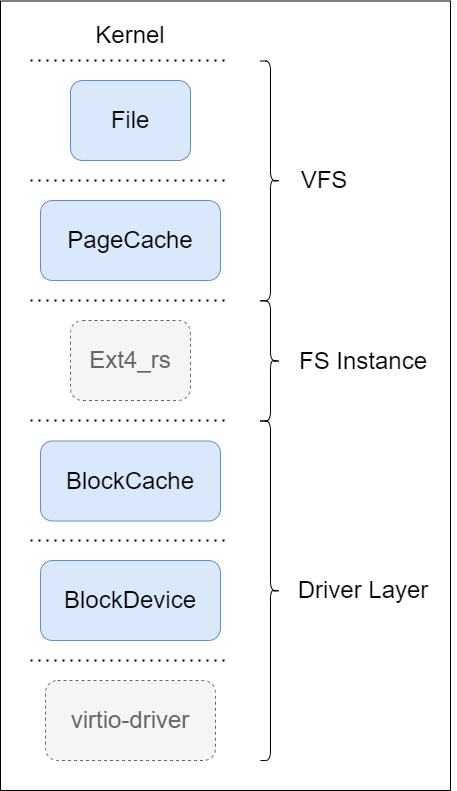
\includegraphics[width=0.5\linewidth]{assets//fs/structure.drawio.png}
    \caption{缓存结构图}
    \label{fig:enter-label}
\end{figure}

\subsubsection{块缓存}
在NoAxiom中,我们使用\code{LruCache}实现了\textbf{异步块缓存}\code{BlockCache},块缓存是驱动的缓存,用于加速驱动设备的读写。
\begin{lstlisting}
pub struct AsyncBlockCache {
    cache: SyncUnsafeCell<LruCache<usize, Arc<[u8; BLOCK_SIZE]>>>,
    block_device: Arc<&'static dyn BlockDevice>,
}

#[async_trait]
impl BlockDevice for AsyncBlockCache {
    fn device_name(&self) -> &'static str {
        "AsyncBlockCache"
    }
    async fn read(&self, id: usize, buf: &mut [u8]) -> DevResult<usize> {
        assert_eq!(buf.len(), BLOCK_SIZE);
        let data = self.read_sector(id).await;
        buf.copy_from_slice(&*data);
        Ok(buf.len())
    }
    async fn write(&self, id: usize, buf: &[u8]) -> DevResult<usize> {
        assert_eq!(buf.len(), BLOCK_SIZE);
        let mut data: [u8; BLOCK_SIZE] = [0; BLOCK_SIZE];
        data.copy_from_slice(buf);
        self.write_sector(id, &data).await;
        Ok(buf.len())
    }
    async fn sync_all(&self) -> DevResult<()> {
        self.sync_all().await;
        Ok(())
    }
}
\end{lstlisting}

其原理便是驱动设备每读取一个块号,都先检查块缓存是否已经存有副本,若有就可以直接从内存中读写,无需经过下层设备I/O操作,写操作需要标记块为\code{Dirty};若发现没有,就可以从内存中读取填充到块缓存中,再进行读写操作。因为块缓存容量有限,若填充时发现需要踢走已有的缓存,就需要考虑写回,我们仅当脏数据时写回。以上高效的设计,为我们的局部性反复读写文件功能提供了良好的性能。

\subsubsection{页缓存}

页缓存和块缓存本质原理是一模一样的,只不过层次不一致,\code{PageCache}缓存的对象是\textbf{文件在内存中打开后读写的信息},它可以加速更上层的请求,比如各类读写类系统调用,如果命中页缓存,就会连具体文件系统都\textbf{不需要访问},\textbf{极大的提高了读写性能}。

\begin{lstlisting}
pub struct Page {
    data: FrameTracker,
    state: PageState,
}

impl Page {
    pub fn new() -> Self {
        unsafe { FRAME_ALLOCS.fetch_add(1, core::sync::atomic::Ordering::SeqCst) };
        Self {
            data: frame_alloc().unwrap(),
            state: PageState::Invalid,
        }
    }
    pub fn as_mut_bytes_array(&self) -> &'static mut [u8] {
        self.data.ppn().get_bytes_array()
    }
    pub fn mark_dirty(&mut self) {
        self.state = PageState::Modified;
    }
}
pub struct PageCache {
    inner: HashMap<usize, Page>,
}
\end{lstlisting}

特别的,我们采用了\textbf{物理页帧}存储海量的页缓存内容,很大程度上缓解了堆栈内存的占用率问题,并且提高了整体的内存利用率。

以下以读操作为例,展示了\code{PageCache}工作的原理:我们会将读请求按照页大小划分,每一页的读,都通过rust中\code{copy_nonoverlapping}的\code{unsafe}方法进行高效的复制;若出现页缺失现象,就会先调用\code{base_read}方法去文件系统中读出,再从页缓存中读出。

\begin{lstlisting}
pub async fn read_at(&self, offset: usize, buf: &mut [u8]) -> SyscallResult {
    ...
    loop {
        let (offset_align, offset_in) = align_offset(current_offset, PAGE_SIZE);
        if let Some(page) = page_cache.get_page(offset_align) {
            ...

            unsafe {
                core::ptr::copy_nonoverlapping(
                    page.as_mut_bytes_array().as_ptr().add(offset_in),
                    buf.as_mut_ptr(),
                    len,
                );
            }

            buf = &mut buf[len..];
            current_offset += len;
            if buf.is_empty() || current_offset == size {
                break;
            }
        } else {
            let new_page = Page::new();
            self.base_read(offset_align, new_page.as_mut_bytes_array())
                .await?;
            page_cache.fill_page(offset_align, new_page);
        }
    }

    Ok((current_offset - offset) as isize)
}
\end{lstlisting}

\subsubsection{路径缓存}
我们在全局上添加了一个由自旋锁保护的路径缓存结构。其内部实现就是一个\code{HashMap},记录了路径字符串到\code{Dentry}结构的映射,主要用于路径解析时的快速查找。

\begin{lstlisting}
lazy_static::lazy_static! {
    pub static ref PATH_CACHE: SpinLock<HashMap<String, Path>> = SpinLock::new(HashMap::new());
}
\end{lstlisting}

如果某文件被\code{close},其路径缓存也不会删掉,这么做的好处在于下次再次碰到该路径可以直接返回一个Negative的\code{Dentry},直到用户显式调用删除文件的系统调用,才会从路径缓存中删去。

\subsubsection{性能对比}

\begin{figure}[H]
    \centering
    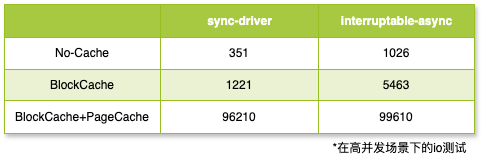
\includegraphics[width=1.0\linewidth]{assets//fs/perf.png}
    \caption{不同条件下高并发场景的性能对比}
    % \label{fig:enter-label}
\end{figure}

\begin{figure}[H]
    \centering
    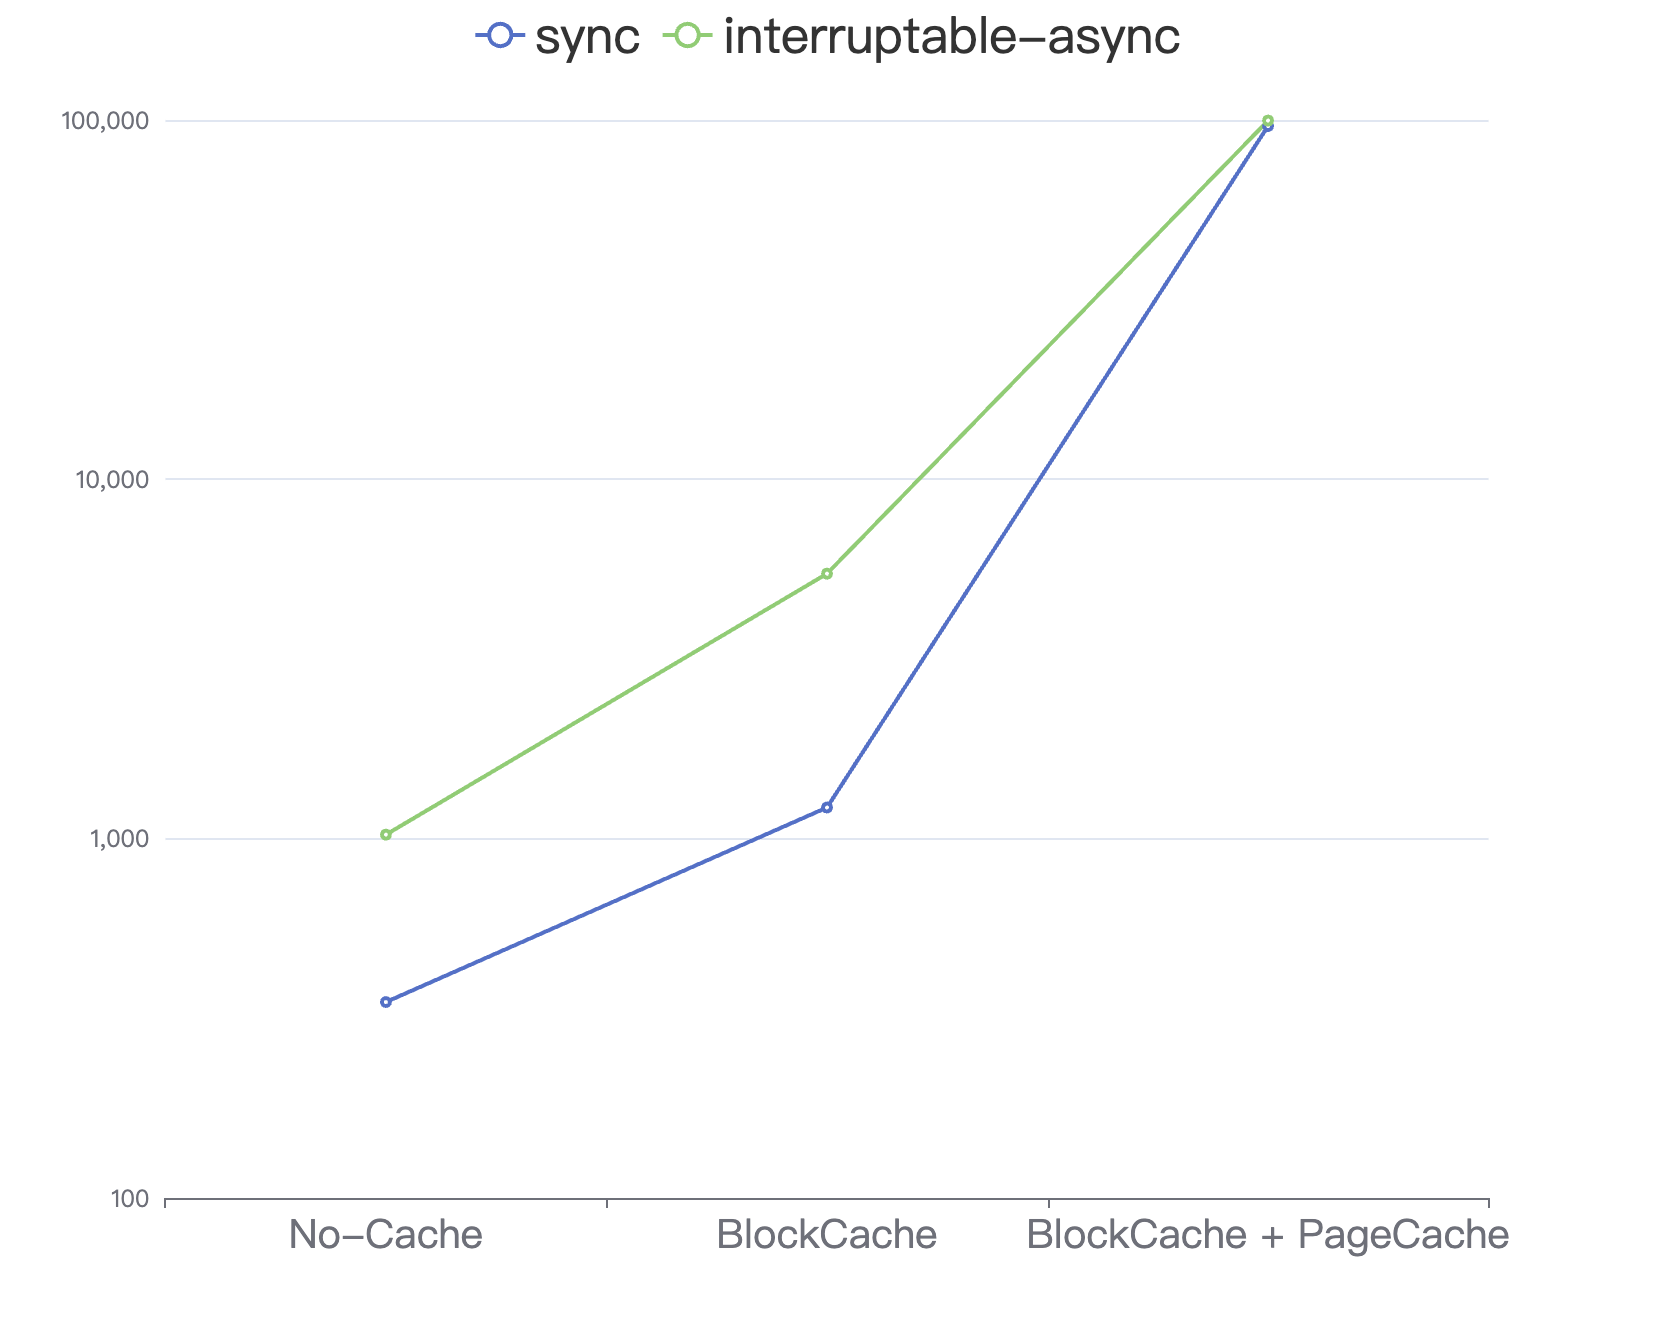
\includegraphics[width=0.7\linewidth]{assets//fs/perf-line.png}
    \caption{不同条件下高并发场景的性能对比-折线图}
    % \label{fig:enter-label}
\end{figure}

以上数字均代表在高并发测试场景下的相对性能,\textbf{越大越好}。我们会发现在没有页缓存的高并发场景下,由异步驱动带来的\textbf{高并发性}使得整体性能优于传统驱动。但在添加了页缓存之后,因为大部分文件已经在内存中得到缓存,操作系统会通过页缓存直接读取,而不需要经过具体文件系统,所有下层的驱动带来的影响就不大了,但整体性能比没有页缓存的实现了\textbf{质的飞跃}。

\begin{figure}[H]
    \centering
    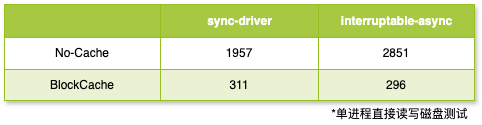
\includegraphics[width=0.7\linewidth]{assets//fs/perf-directly-on-disk.png}
    \caption{单进程磁盘读写性能}
    % \label{fig:enter-label}
\end{figure}\begin{figure}[H]
    \centering
    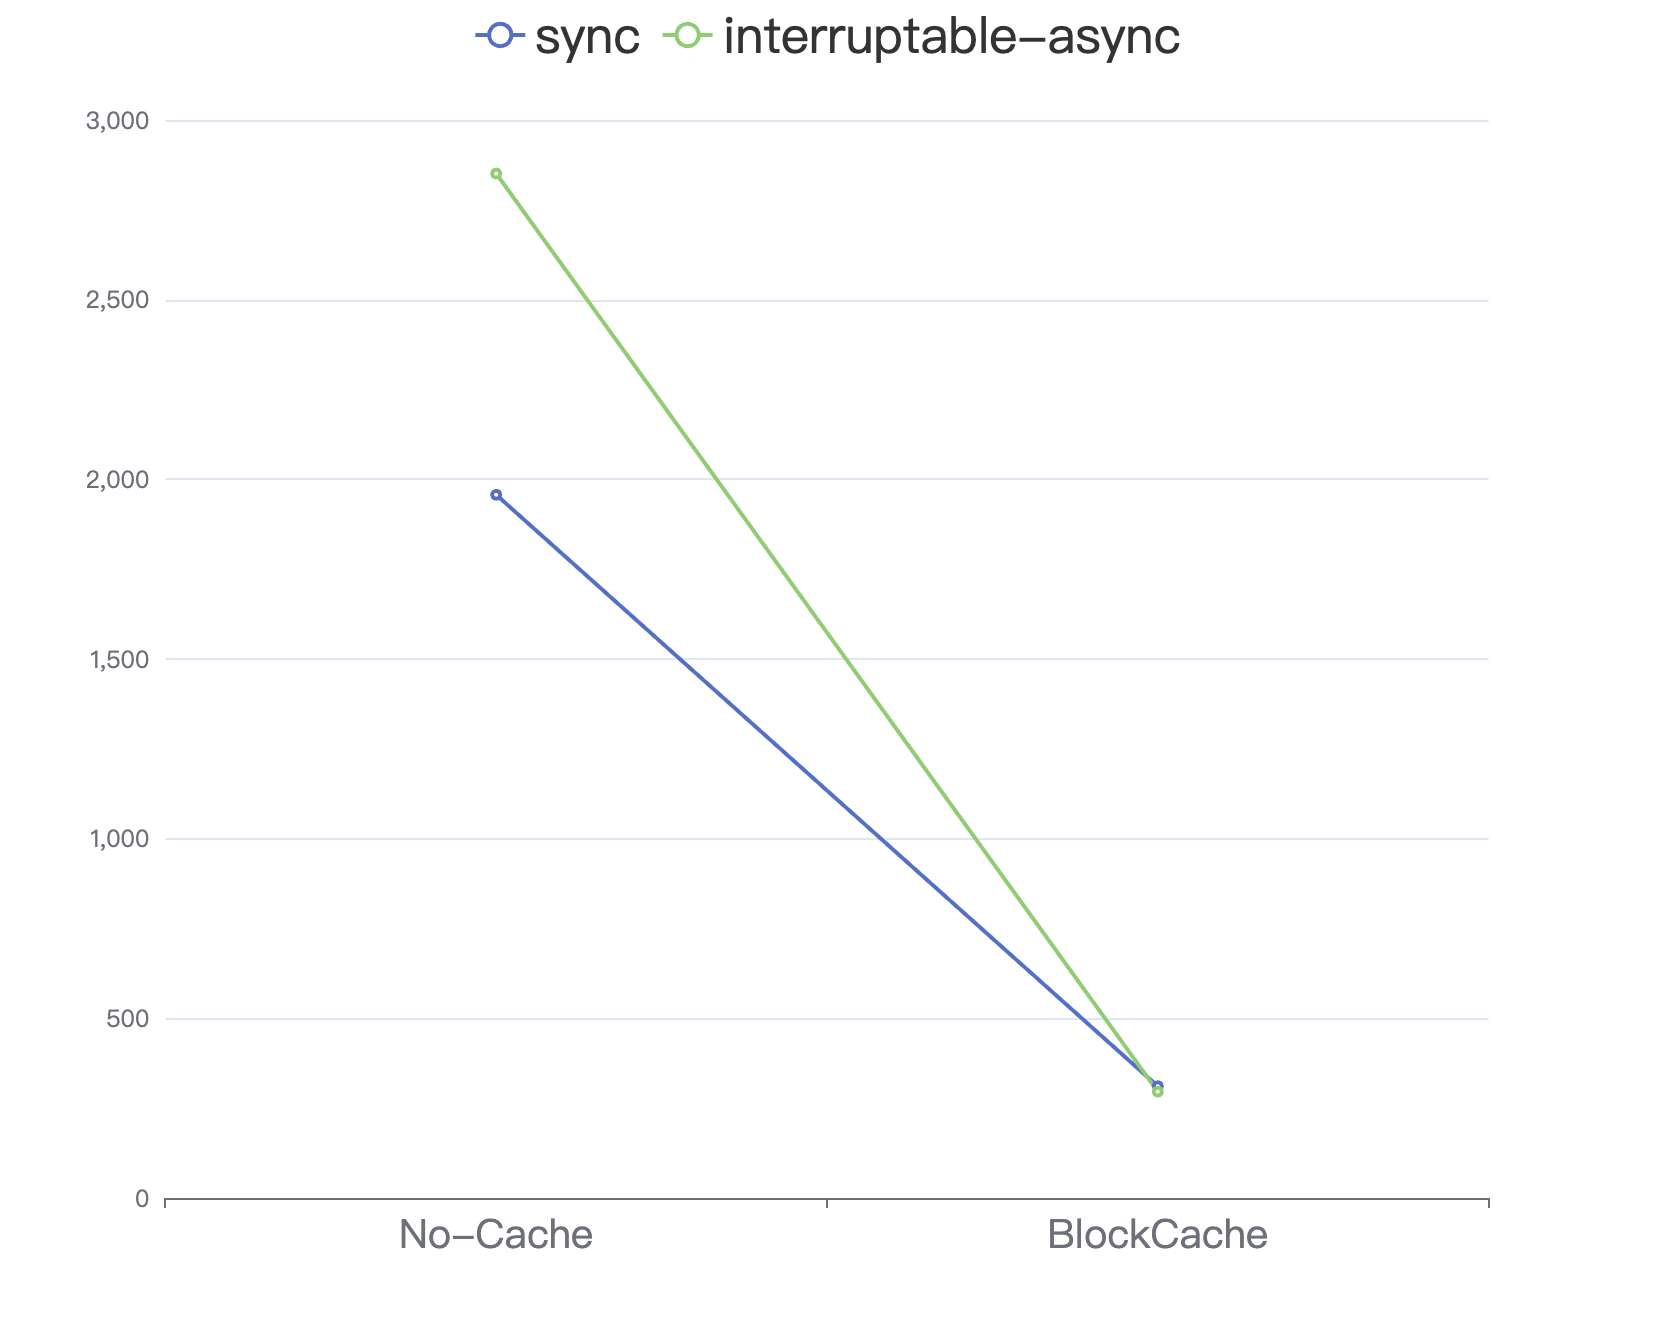
\includegraphics[width=0.7\linewidth]{assets//fs/perf-directly-on-disk-line.png}
    \caption{单进程磁盘读写性能-折线图}
    % \label{fig:enter-label}
\end{figure}

我们还测试了一般场景下的读写性能,上面两个图描述了反复读写一片连续扇区时的时间消耗,\textbf{越小越好}。我们会发现在这种普通的单进程场景下,传统驱动表现反而比NoAxiom的异步驱动更好,原因就在于我们的异步驱动在单进程场景下仍然会让权,但此时调度器没有别的任务可以调度,只能继续调度本进程,这样反而造成了\textbf{时间粒度更大}的忙等,这里的时间粒度指的就是异步调度器执行一次完整调度过程的开销,在这期间是无法立即响应的。而传统驱动通过平凡的\code{loop}反而可以实现更快的响应。

但在加上块缓存优化后,因为是对于连续磁盘块的性能测试,此时块缓存就会缓存这些盘块,不管底层驱动是何种实现,大部分情况下都可以直接从块缓存中得到数据,也就导致了两种驱动的性能差距不大。

\begin{figure}[H]
    \centering
    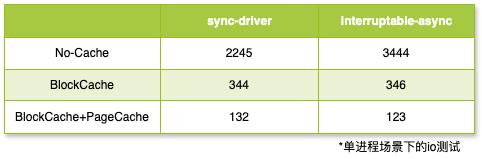
\includegraphics[width=0.7\linewidth]{assets//fs/perf-single-file.png}
    \caption{单进程反复读写场景}
    % \label{fig:enter-label}
\end{figure}\begin{figure}[H]
    \centering
    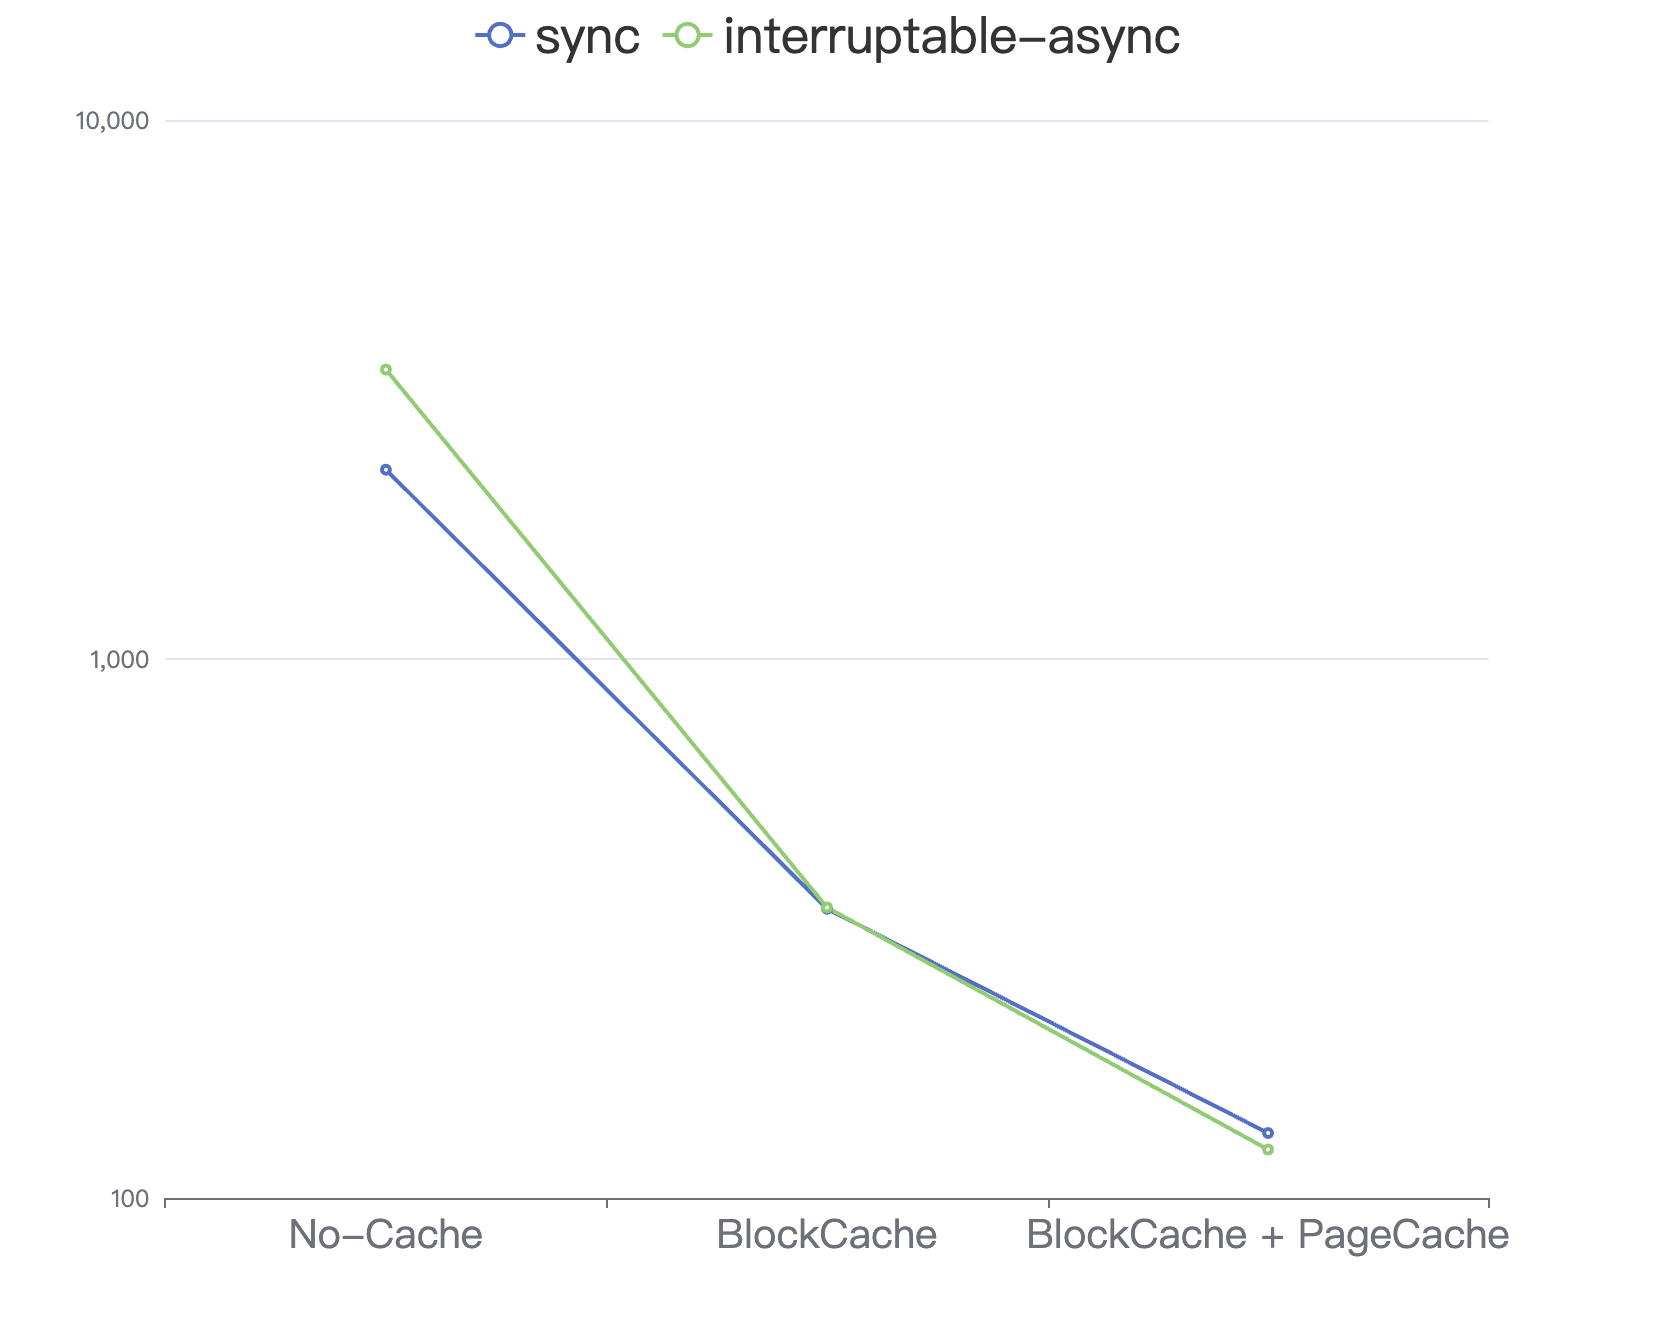
\includegraphics[width=0.7\linewidth]{assets//fs/perf-single-file-line.png}
    \caption{单进程反复读写场景-折线图}
    % \label{fig:enter-label}
\end{figure}

以上两个图,更加综合的展示了块缓存和页缓存的适用场景和功能。它描述了单进程环境下反复读写文件的时间消耗,\textbf{越小越好}。在没有缓存的情况下,传统驱动反而比异步驱动优秀;在有块缓存或者页缓存的情况下,两者区别就不大了。

\subsection{文件系统实例}
\subsubsection{具体文件系统EXT4/FAT32}
我们为两种文件系统格式实现了上述\code{trait},其中Ext4文件系统,区别于往届传统队伍的lwext4库实现,我们使用了\textbf{自主fork}的ext4\_rs\footnote{https://github.com/yuoo655/ext4\_rs}库,这是一个基于rust实现的\textbf{异步文件系统}\footnote{https://github.com/YuXuaann/ext4\_rs-async-smp},提供了原库中所有支持操作的异步版本。

\begin{figure}[H]
    \centering
    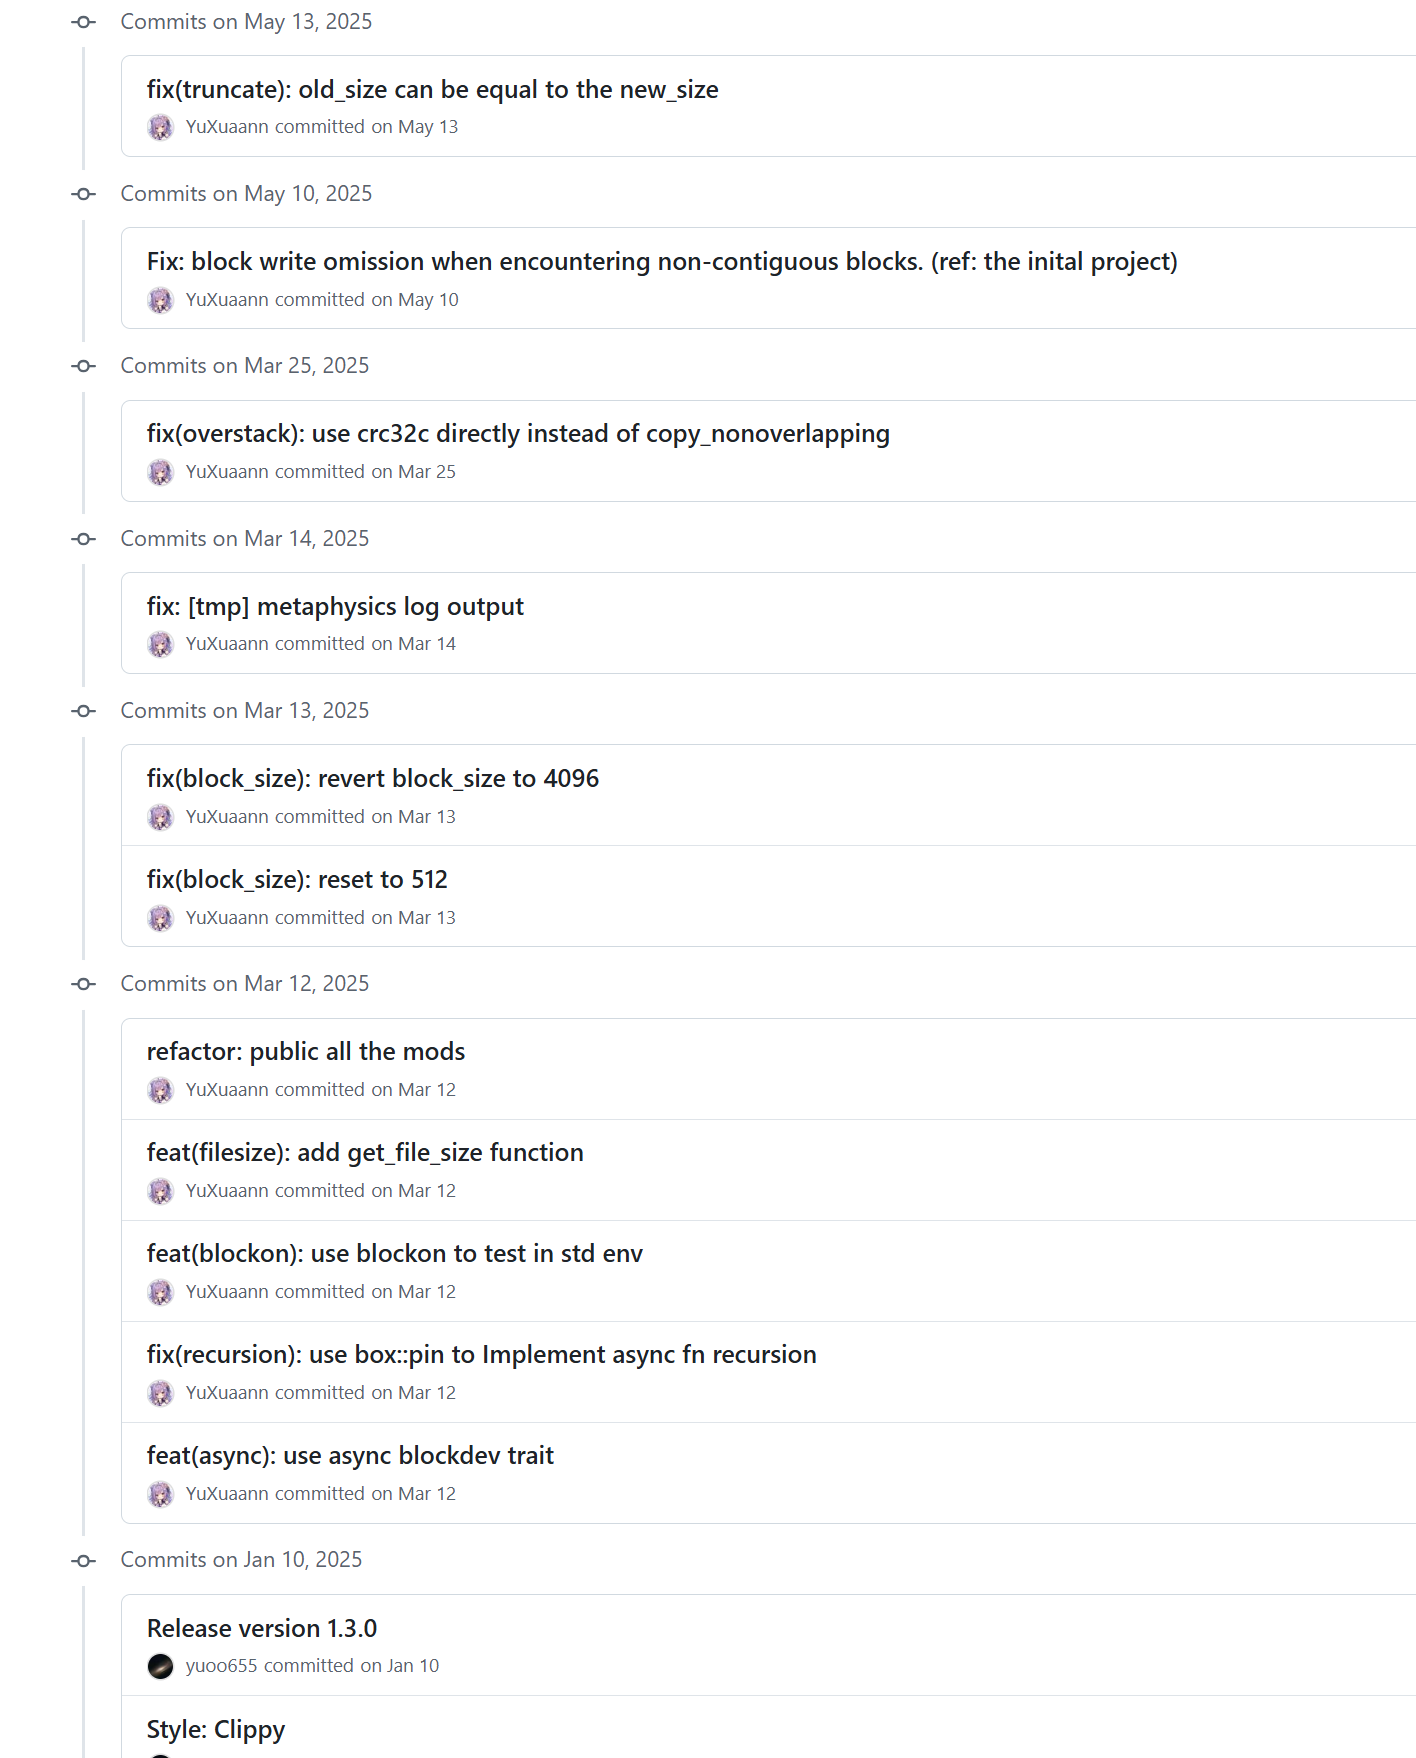
\includegraphics[width=0.8\linewidth]{assets//fs/image.png}
    \caption{ext4\_rs-async库的适配记录}
    % \label{ext4\_rs-async库的适配记录}
\end{figure}

\subsubsection{管道文件}
管道为进程(尤其是父子进程)之间的通信提供了良好的方法。其本质是一个\textbf{生产者-消费者问题},我们需要解决多消费者和多生产者的互斥访问。

\begin{figure}[H]
    \centering
    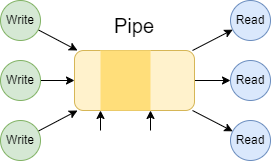
\includegraphics[width=0.8\linewidth]{assets//fs/管道pipedrawio.drawio.png}
    \caption{管道}
    \label{管道}
\end{figure}

在传统内核的实现中,对于管道的访问采取“有多少读多少”,“能写多少写多少”的策略,进程之间不存在联系,只考虑当前管道中的内容,对于读请求如果管道为空就直接返回0,对于写请求也是如果管道已满就返回零。因为用户程序的行为往往是通过循环等到足够的内容或空间进行读写,所以传统内核的做法导致了非常多空效果的系统调用,并且产生了大量切换特权态造成的上下文开销。

针对以上传统内核的弊端,NoAxiom基于无栈协程机制设计了\textbf{让权-唤醒}机制的管道虚拟文件系统。我们为其实现了VFS的所有\code{trait},并且在创建新文件时,会\textbf{虚拟挂载}在根目录下,为其\code{inode}标记\code{FIFO}。

\begin{lstlisting}
pub struct PipeDentry {
    meta: DentryMeta,
}

impl PipeDentry {
    /// we mount all the pipes to the root dentry
    pub fn new(name: &str) -> Arc<Self> {
        let parent = root_dentry();
        let super_block = parent.super_block();
        let pipe_dentry = Arc::new(Self {
            meta: DentryMeta::new(Some(parent.clone()), name, super_block),
        });
        debug!("[PipeDentry] create pipe dentry: {}", pipe_dentry.name());
        parent.add_child_directly(pipe_dentry.clone());
        pipe_dentry
    }
}
\end{lstlisting}

对于一个管道读写请求,我们首先会检查管道Buffer中是否存在可供读写的内容,若没有,则将当前进程的\code{Waker}存到\code{PipeBuffer}结构体中,然后在\code{Future}中返回\code{Pending}让权。

\begin{lstlisting}
struct PipeReadFuture {
    read_len: usize,
    pipe_buffer: Arc<SpinLock<PipeBuffer>>,
}
impl Future for PipeReadFuture {
    // just for error handling
    type Output = SysResult<()>;

    fn poll(self: Pin<&mut Self>, cx: &mut Context<'_>) -> Poll<Self::Output> {
        let mut buffer = self.pipe_buffer.lock();
        if buffer.write_end {
            if buffer.read_available() {
                Poll::Ready(Ok(()))
            } else {
                buffer.add_read_event(self.read_len, cx.waker().clone());
                Poll::Pending
            }
        } else {
            Poll::Ready(Ok(()))
        }
    }
}
\end{lstlisting}

若管道Buffer中存在可供读写的内容,首先进行管道的读写操作,然后唤醒存在\code{PipeBuffer}中的\code{Waker}。这里在往届队伍中存在一种简单设计,即唤醒全部\code{Waker}。我们在这里创新地设计了\textbf{按需唤醒}机制,我们只唤醒当前\code{PipeBuffer}中可用长度下能够唤醒的所有\code{Waker}。因为每一个管道读写请求均存在长度参数,我们在存\code{Waker}的过程中还会一起记录此次读写请求的长度参数,当一次管道读写操作完成时,就会遍历\code{Waker}队列,pop出管道\code{Buffer}长度可以cover住的\code{Waker}唤醒。

\begin{lstlisting}
impl PipeBuffer {
    fn notify_read_waker(&mut self) {
        let mut read_available = self.read_available_len();
        if read_available == 0 {
            return;
        }
        while let Some((len, waker)) = self.read_wakers.pop() {
            if read_available >= len {
                read_available -= len;
                waker.wake();
            } else {
                waker.wake();
                break;
            }
        }
    }
}

#[async_trait]
impl File for PipeFile {
    async fn base_read(&self, _offset: usize, buf: &mut [u8]) -> SyscallResult {
        PipeReadFuture::new(buf.len(), self.buffer.clone()).await?;
        let mut buffer = self.buffer.lock();
        let ret = buffer.read(buf);
        if ret != 0 {
            buffer.notify_write_waker();
        }
        Ok(ret as isize)
    }
}
\end{lstlisting}

总而言之,NoAxiom的基于无栈协程机制的\textbf{让权-唤醒}机制,保证了不存在读写长度为0的管道读写系统调用,大大\textbf{减少了上下文切换开销}和系统调用数量。

顺带一提,NoAxiom中提供给管道使用的Buffer,是独立实现的\code{RingBuffer}结构,并且创新地采用了\textbf{物理页帧}进行存储,极大地避免了堆栈空间的占用。

\begin{lstlisting}
/// Ring buffer that max size is PIPE_BUF_SIZE
struct PipeBuffer {
    data: FrameTracker,
    head: usize,
    tail: usize,
    status: PipeBufferStatus,
    read_wakers: Vec<(usize, Waker)>,
    write_wakers: Vec<(usize, Waker)>,
    read_end: bool,
    write_end: bool,
}
\end{lstlisting}

\subsubsection{套接字文件}
首先,我们提供了枚举类\code{Sock},用来分发不同socket。

\begin{lstlisting}
pub enum Sock {
    Tcp(TcpSocket),
    Udp(UdpSocket),
    // Unix(UnixSocket),
}

impl Sock {
    pub fn bind(&mut self, addr: SockAddr, fd: usize) -> SysResult<()> {
        let endpoint = addr.get_endpoint();
        match self {
            Sock::Tcp(socket) => socket.bind(endpoint, fd),
            Sock::Udp(socket) => socket.bind(endpoint, fd),
        }
    }
    pub fn listen(&mut self, backlog: usize) -> SysResult<()> {
        match self {
            Sock::Tcp(socket) => socket.listen(backlog),
            _ => Err(Errno::ENOSYS),
        }
    }
    // 下同
    pub async fn connect(&mut self, addr: SockAddr) -> SysResult<()>
    pub async fn accept(&mut self) -> SysResult<(TcpSocket, IpEndpoint)>
    pub fn setsockopt(&mut self, level: usize, optname: usize, optval: &[u8]) -> SysResult<()>
    pub fn meta(&self) -> &SocketMeta
    pub fn local_endpoint(&self) -> Option<IpEndpoint>
    pub fn peer_endpoint(&self) -> Option<IpEndpoint>
    pub async fn read(&mut self, buf: &mut [u8]) -> (SysResult<usize>, Option<IpEndpoint>)
    pub async fn write(&mut self, buf: &[u8], remote: Option<IpEndpoint>) -> SysResult<usize>
    pub fn shutdown(&mut self, operation: ShutdownType) -> SysResult<()>
}
\end{lstlisting}

然后我们通过\code{AsyncMutex}异步锁,包裹\code{Sock}结构体,就构成了套接字文件结构体。我们也将其视作普通文件,为其实现一系列标准的接口。

\begin{lstlisting}
pub struct SocketFile {
    meta: FileMeta,
    sock: AsyncMutex<Sock>,
    type_: PosixSocketType,
}

unsafe impl Send for SocketFile {}
unsafe impl Sync for SocketFile {}

#[async_trait]
impl File for SocketFile {
    fn meta(&self) -> &FileMeta {
        &self.meta
    }
    async fn base_read(&self, _offset: usize, buf: &mut [u8]) -> SyscallResult {
        let mut sock = self.socket().await;
        let res;
        match &mut *sock {
            Sock::Tcp(socket) => {
                res = socket.read(buf).await.0?;
            }
            Sock::Udp(socket) => {
                res = socket.read(buf).await.0?;
            }
        }

        Ok(res as isize)
    }
    async fn base_write(&self, _offset: usize, buf: &[u8]) -> SyscallResult {
        let mut sock = self.socket().await;
        let res;
        match &mut *sock {
            Sock::Tcp(socket) => {
                res = socket.write(buf, None).await?;
            }
            Sock::Udp(socket) => {
                // use its remote endpoint as the destination
                res = socket.write(buf, None).await?;
            }
        }

        Ok(res as isize)
    }
    fn poll(&self, req: &PollEvent, waker: Waker) -> PollEvent {
        let mut sock = block_on(self.socket());
        let poll_res = match &mut *sock {
            Sock::Tcp(socket) => socket.poll(req, waker),
            Sock::Udp(socket) => socket.poll(req, waker),
        };

        let mut res = PollEvent::empty();
        if poll_res.contains(PollEvent::POLLIN) {
            res |= PollEvent::POLLIN;
        }
        if poll_res.contains(PollEvent::POLLOUT) {
            res |= PollEvent::POLLOUT;
        }
        if poll_res.contains(PollEvent::POLLHUP) {
            warn!("[Socket::poll] PollEvent is hangup");
            res |= PollEvent::POLLHUP;
        }
        res
    }
}
\end{lstlisting}

套接字文件和管道文件一样,也提供了\textbf{虚拟挂载}在根目录的功能。关于套接字文件具体的功能实现,在后文的网络模块中有详细阐述。

\subsubsection{基于内存的文件系统 RamFs}
RamFs是建立在内存上的非持久文件系统,使用堆内存创建的\code{Vec}去存储文件的内容。该文件系统目前仅用来实现部分虚拟文件,用于满足用户交互的需求。具有响应速度快的优势。

\subsection{虚拟文件}
凭借完善的VFS结构设计,下面的各类文件实例,只需要实现相应的\code{trait}即可。

\subsubsection{进程管理 /proc}
\code{/proc}用来存储内核当前的运行状态,用户可以通过\code{\proc}目录下的文件查看当前正在运行进程的信息,也可以通过与这些文件交互实现和内核进程的直接交互。

\begin{enumerate}
    \item \code{/proc/meminfo}: 读取时返回内存信息。
    \item \code{/proc/mounts}: 读取时返回挂载的文件系统信息。
    \item \code{/proc/sys/}: 基于RamFs,存储关于系统相关文件信息。
    \item \code{/proc/sys/kernel/pid_max}: 基于RamFs,读取时返回最大进程号。
    \item \code{/proc/self/}: 基于RamFs,存储关于当前进程相关信息。
    \item \code{/proc/self/exe}: 代表当前程序,用\code{readlink}读取时返回当前程序的绝对路径
\end{enumerate}

\subsubsection{虚拟设备 /dev}
\code{/dev}用来存储那些代表硬件设备的文件,它允许用户使用与文件交互的方式与硬件交互。

\begin{enumerate}
    \item \code{/dev/null}: 垃圾桶。读操作返回空,写操作相当于丢弃数据。
    \item \code{/dev/zero}: 读取时会返回全0.
    \item \code{/dev/tty}: 非常重要的字符设备。它代表当前正在使用的控制终端设备,目前也是我们内核的串口设备,这意味着实际上每个进程初始化时\code{FdTable}中默认的\code{STDIN}、\code{STDOUT}、\code{STDERR}的实际实现都是\code{TtyFile}。
    \item \code{/dev/rtc}: 读取时返回实时时钟。
    \item \code{/dev/cpu_dma_latency}: 读取时返回CPU的DMA延迟。
    \item \code{/dev/urandom}: 读取时返回随机数。
    \item \code{/dev/shm}: 用于实现进程间的共享内存。
\end{enumerate}


\subsection{系统调用实现}
\subsubsection{I/O读写类}
上面在缓存中已经介绍了大致的读写操作。但在实际读写系统调用中,我们还需要通过信号机制中提供的\code{intable}接口,为那些可能产生阻塞的读写操作(例如\code{socket}读写或管道读写)提供强制退出的可能。
\subsubsection{I/O多路复用}
在\code{File}结构体中,我们强制要求每一个文件都需要实现\code{poll}方法,就是为了优雅的实现I/O的多路复用功能。通过rust强大的\code{trait}功能,我们只需要使用VFS层提供的抽象接口,便可实现对\textbf{所有}文件(可以是各种不同类型的文件)的多路监听。

其中\code{poll}方法原型是这样定义的:
\begin{lstlisting}
fn poll(&self, req: &PollEvent, waker: Waker) -> PollEvent;
\end{lstlisting}
它会传入当前进程的\code{Waker},以及\code{poll}操作的具体请求,具体文件需要返回\code{poll}请求中它可以接受处理的那些请求。如果某些请求暂时还无法得到处理,具体文件就会将当前进程的\code{Waker}存入它内部的\code{Buffer}中。

对于具体系统调用来说,如果它观察到文件list中无一准备就绪,调度器就会执行让权操作,执行其他进程的任务,直到具体文件唤醒原进程。以上操作只需要实现\code{Future trait}即可实现,这样的思路完美利用了无栈协程机制,以\textbf{高效优雅}的方式实现了I/O多路复用功能。

\begin{lstlisting}
pub struct PpollItem {
    id: usize,
    events: PollEvent,
    file: Arc<dyn File>,
}

pub struct PpollFuture {
    fds: Vec<PpollItem>,
}

impl Future for PpollFuture {
    type Output = Vec<(usize, PollEvent)>;

    fn poll(self: Pin<&mut Self>, cx: &mut Context<'_>) -> Poll<Self::Output> {
        let mut result = Vec::new();
        for poll_item in &self.fds {
            let id = poll_item.id;
            let req = &poll_item.events;
            let res = poll_item.file.poll(req, cx.waker().clone());
            if !res.is_empty() {
                result.push((id, res));
            }
        }
        if result.is_empty() {
            Poll::Pending
        } else {
            Poll::Ready(result)
        }
    }
}
\end{lstlisting}

特别的,我们对于系统调用\code{sys_pselect}也\textbf{复用}了上述\code{Future}实现。

\subsection{其他相关结构}
\subsubsection{文件描述符表 FdTable}
每一个进程都拥有一个文件描述符表。因为在用户的视角,文件是一个抽象的概念,用户是通过文件描述符\code{fd}(一个非负整数)来操控文件的,而内核中进程持有的文件描述符表就是维护这一映射关系的结构。\code{FdTable}记录了每一个\code{fd}对应的文件及其\code{FcntlArgFlags}。在进程\code{fork}时,文件描述符表会完整复制,我们只需要为\code{FdTable}标记\code{\#[derive(Clone)]}就可以优雅地自动实现\code{Fdtable}复制方法。

\begin{lstlisting}
#[derive(Clone)]
pub struct FdTableEntry {
    flags: FcntlArgFlags,
    pub file: Arc<dyn File>,
}

#[derive(Clone)]
pub struct FdTable {
    pub table: Vec<Option<FdTableEntry>>,
    rlimt: RLimit,
}
\end{lstlisting}

其中\code{FcntlArgFlags}结构主要是用来标记该文件描述符是否拥有\code{close_on_exec}标志位,该标志位可以保证这个文件描述符在执行了\code{sys_execve}后被关闭,防止出现安全问题。

\code{FdTable}还承担了对于\code{RLimit}的管理:
\begin{lstlisting}
/// Resource Limit from linux
#[derive(Debug, Clone, Copy)]
pub struct RLimit {
    /// Soft limit
    pub rlim_cur: usize,
    /// Hard limit (ceiling for rlim_cur)
    pub rlim_max: usize,
}
\end{lstlisting}

若\code{alloc}操作申请的\code{fd}超过了最大描述符数量的限制,便会返回\code{Errno::EMFILE}。除此之外,也为系统调用\code{sys_prlimit}提供了设置当前进程文件描述符的\code{RLlimit}接口: 

\begin{lstlisting}
pub fn rlimit_mut(&mut self) -> &mut RLimit {
    &mut self.rlimt
}

pub async fn sys_prlimit64(
    &self,
    pid: usize,
    resource: u32,
    new_limit: usize,
    old_limit: usize,
) -> SyscallResult {
    let task = ...
    let mut fd_table = task.fd_table();
    let new_limit = UserPtr::<RLimit>::new(new_limit);
    ...
    if !new_limit.is_null() {
        match resource {
            Resource::NOFILE => *fd_table.rlimit_mut() = new_limit.read().await?,
            _ => {}
        }
    }
    Ok(0)
}
\end{lstlisting}

为充分利用内存资源和提高内核效率,若用户使用了\code{sys_close}关闭了某个文件描述符\code{fd}对应的文件,那么该\code{fd}对应的槽位将仅需要设置为\code{None},性能开销极小。下次申请\code{fd}时会优先选择空槽位,提高了内存的利用率。

\begin{lstlisting}
/// get the soft rlimit of the fd table
fn rslimit(&self) -> usize {
    self.rlimt.rlim_cur
}

/// Allocate a new fd slot, if has empty slot, return the first empty slot,
/// you should use tht fd after alloc immediately
pub fn alloc_fd(&mut self) -> SysResult<usize> {
    if let Some(fd) = self.table.iter().position(|x| x.is_none()) {
        return Ok(fd);
    }

    if self.table.len() >= self.rslimit() {
        Err(Errno::EMFILE)
    } else {
        self.table.push(None);
        Ok(self.table.len() - 1)
    }
}
\end{lstlisting}

\subsection{文件一致性管理}
在\code{Inode}生命周期结束时,会将\code{PageCache}写回;在系统\code{Shutdown}时,显式调用\code{sync}方法,写回脏数据。

\newpage
\section{信号系统}
\subsection{信号管理}

$\blacktriangleright$\textbf{待处理信号管理}

NoAxiom使用\code{PendingSigs}维护等待处理的信号,其内部维护了当前进程对应的待处理信号信息。

\begin{lstlisting}
pub struct SigPending {
    pub sig_mask: SigMask,        // signal mask of the task
    pub queue: VecDeque<SigInfo>, // pending signal queue that should be handled
    pub pending_set: SigSet,      // current pending signal set
    pub should_wake: SigSet,      // signals that should wake the task
}
\end{lstlisting}

我们使用\code{SpinLock}自旋锁保护\code{PendingSigs},使其访问具备原子性。

$\blacktriangleright$\textbf{信号捕获函数管理}

我们使用\code{SigAction}对于某一信号的具体处理逻辑进行管理。其中\code{SAHandlerType}字段给定了当前处理函数由用户定义还是执行默认操作,若由用户定义,则在检查信号时会进行用户信息的准备。

\begin{lstlisting}
pub struct KSigAction {
    pub handler: SAHandlerType,
    pub mask: SigMask,
    pub flags: SAFlags,
    pub restorer: usize,
}
\end{lstlisting}

$\blacktriangleright$\textbf{信号具体信息维护}

为了便于维护信号信息,我们使用\code{SigInfo}对于信号传递的信息进行了详细描述。其中包括了:信号编号、信号类型、信号错误码、信号详细信息等信息。其中\code{detail}表示了信号详细信息,如\code{SIG_KILL}发生时,我们将通过该字段传递发送该信号的具体进程,以此便于内核检查。

\begin{lstlisting}
pub struct SigInfo {
    pub signo: Signo,
    pub code: SigCode,
    pub errno: SigErrno,
    pub detail: SigDetail,
}
\end{lstlisting}

\subsection{信号处理流程}

$\blacktriangleright$\textbf{信号检测}

在任务运行的主函数\code{task_main}中,在执行完用户系统调用后,我们会对于当前进程待处理的信号进行检测。其具体处理逻辑为:检查是否具有等待处理的信号,并访问当前进程的\code{SigAction}进行具体的信号处理。假如当前的\code{SigAction}由用户定义,那么还需要进行对应的用户上下文与用户栈信息的更新。

\begin{lstlisting}
task.check_signal(None).await;
\end{lstlisting}

$\blacktriangleright$\textbf{信号返回}

当需要执行\code{sigreturn}系统调用时,由于需要在用户态执行系统调用,因此需要对于对应跳板页进行用户空间的映射。我们在地址空间初始化的时候就对于该页面进行了映射。具体返回时,我们将根据不同的架构内嵌一段汇编代码指示用户进行返回。

\begin{lstlisting}
.section  .text.signal
.globl    user_sigreturn
.align    12
user_sigreturn:
ori       $a7, $zero, 139          # syscall SIGRETURN
syscall   0
\end{lstlisting}

\subsection{可中断系统调用}

Linux中规定了部分系统调用可被特定信号打断,如\code{futex}、\code{ppoll}等调用均会在调用过程中接受信号时,返回错误码\code{Errno::EINTR},以防进程因系统调用永久挂起而导致进程卡死。

为了统一规范该行为,NoAxiom中设计了\code{intable(future)}函数用于进行可打断操作的异步状态机构建。具体而言,调用该函数时,会将原有的异步操作在外部进一步包装为\code{IntableFuture},该异步函数会在内部\code{future}返回\code{Pending}的时候,检测当前进程的信号状态,假如检测到存在等待处理的信号,则直接返回\code{Errno::EINTR}用于指示当前异步函数被打断。

\begin{lstlisting}
impl<F, T> Future for IntableFuture<'_, F>
where F: Future<Output = T>
{
    type Output = SysResult<T>;
    fn poll(self: Pin<&mut Self>, cx: &mut Context<'_>) -> Poll<Self::Output> {
        let this = self.project();
        let task = this.task;
        match this.fut.poll(cx) {
            Poll::Ready(res) => Poll::Ready(Ok(res)),
            Poll::Pending => {
                if task.peek_has_pending_signal(this.mask) {
                    Poll::Ready(Err(Errno::EINTR))
                } else {
                    Poll::Pending
                }
            }
        }
    }
}
\end{lstlisting}

例如,在\code{ppoll}实现中,我们使用\code{intable}包装了原有的轮询操作,使其变为可打断形式,并通过\code{intable.await?}实现了错误码的传回。

\begin{lstlisting}
// ppoll
let intable = intable(self.task, fut, None);
let res = match intable.await? {
    TimeLimitedType::Ok(res) => res,
    TimeLimitedType::TimeOut => return Ok(0),
};
\end{lstlisting}

% \newpage
% \section{时钟模块}

\newpage
\section{网络模块}

\subsection{结构概述}

\begin{figure}[H]
    \centering
    \includegraphics[width=1\linewidth]{assets/net/struct.png}
    \caption{网络结构}
    \label{网络结构}
\end{figure}

我们首先设计了\code{Socket trait}用来抽象不同类型套接字的行为(后文会有这些\code{trait}实现的详细阐述),当然大部分操作使用了异步让权方法以提高CPU利用率:

\begin{lstlisting}
/// TCP/UDP or other socket should implement this trait
#[async_trait]
pub trait Socket: Send + Sync + DowncastSync {
    /// Read data from the socket.
    ///
    /// `buf` is the buffer to store the read data
    ///
    /// return:
    /// - Success: (Returns the length of the data read, the endpoint
    /// from which data was read).
    /// - Failure: Error code
    async fn read(&self, buf: &mut [u8]) -> (SysResult<usize>, Option<IpEndpoint>);

    /// Write data to the socket.
    ///
    /// `buf` is the data to be written  
    /// `to` is the destination endpoint. If None, the written data will be
    /// discarded.
    ///
    /// return: the length of the data written
    async fn write(&self, buf: &[u8], to: Option<IpEndpoint>) -> SysResult<usize>;

    /// The bind() function is used to associate a socket with a particular IP
    /// address and port number on the local machine.
    ///
    /// return: whether the operation is successful
    fn bind(&mut self, local: IpEndpoint, fd: usize) -> SysResult<()>;

    /// `backlog` is the maximum length to which the queue of pending
    /// connections
    ///
    /// return: whether the operation is successful
    fn listen(&mut self, backlog: usize) -> SysResult<()>;

    /// It is used to establish a connection to a remote server.
    /// When a socket is connected to a remote server,
    /// the operating system will establish a network connection with the server
    /// and allow data to be sent and received between the local socket and the
    /// remote server.
    ///
    /// return: whether the operation is successful
    async fn connect(&mut self, remote: IpEndpoint) -> SysResult<()>;

    /// It is used to accept a new incoming connection.
    ///
    /// only used for TCP
    async fn accept(&mut self) -> SysResult<(TcpSocket, IpEndpoint)>;

    /// It is used to send data to a connected socket.
    ///
    /// return: whether the operation is successful
    fn shutdown(&mut self, operation: ShutdownType) -> SysResult<()>;

    /// Get the socket's metadata
    #[allow(unused)]
    fn meta(&self) -> &SocketMeta;

    /// It is used to get the local endpoint of the socket.
    fn local_endpoint(&self) -> Option<IpEndpoint>;

    /// It is used to get the remote endpoint of the socket.
    fn peer_endpoint(&self) -> Option<IpEndpoint>;

    fn setsockopt(&self, _level: usize, _optname: usize, _optval: &[u8]) -> SysResult<()> {
        Ok(())
    }
}
\end{lstlisting}

在实现网络的系统调用时,只需要调用以上方法即可。在此基础上,根据Linux哲学“万物皆文件”,我们对各类\code{Socket}进行了一层包装,给内核提供了\code{SocketFile}结构:

\begin{lstlisting}
pub struct TcpSocket {
    meta: SocketMeta,
    state: TcpState,
    handles: Vec<SocketHandle>,
    local_endpoint: Option<IpEndpoint>,
}
pub struct UdpSocket {
    pub handle: SocketHandle,
    remote_endpoint: Option<IpEndpoint>,
    meta: SocketMeta,
}

pub enum Sock {
    Tcp(TcpSocket),
    Udp(UdpSocket),
    // Unix(UnixSocket),
}

/// The file for socket
pub struct SocketFile {
    meta: FileMeta,
    sock: AsyncMutex<Sock>,
    type_: PosixSocketType,
}
\end{lstlisting}

类似于前文所述的EXT4文件系统,我们通过对实际文件包裹了一层\code{AsyncMutex},让其支持在\textbf{异步环境下的互斥访问}。然后为它实现了\code{File trait},包括普通的读写以及支持I/O多路复用功能,从而以\textbf{非常高效的开发效率}接入了文件系统,并且也不需要改动任何的常规读写系统调用。

\begin{lstlisting}
#[async_trait]
impl File for SocketFile {
    fn meta(&self) -> &FileMeta {
        &self.meta
    }
    async fn base_read(&self, _offset: usize, buf: &mut [u8]) -> SyscallResult {
        let mut sock = self.socket().await;
        let res;
        match &mut *sock {
            Sock::Tcp(socket) => {
                res = socket.read(buf).await.0?;
            }
            Sock::Udp(socket) => {
                res = socket.read(buf).await.0?;
            }
        }
        Ok(res as isize)
    }
    async fn base_write(&self, _offset: usize, buf: &[u8]) -> SyscallResult {
        let mut sock = self.socket().await;
        let res;
        match &mut *sock {
            Sock::Tcp(socket) => {
                res = socket.write(buf, None).await?;
            }
            Sock::Udp(socket) => {
                res = socket.write(buf, None).await?;
            }
        }
        Ok(res as isize)
    }
    ...
    fn poll(&self, req: &PollEvent, waker: Waker) -> PollEvent {
        let mut sock = block_on(self.socket());
        let poll_res = match &mut *sock {
            Sock::Tcp(socket) => socket.poll(req, waker),
            Sock::Udp(socket) => socket.poll(req, waker),
        };

        let mut res = PollEvent::empty();
        if poll_res.contains(PollEvent::POLLIN) {
            res |= PollEvent::POLLIN;
        }
        if poll_res.contains(PollEvent::POLLOUT) {
            res |= PollEvent::POLLOUT;
        }
        if poll_res.contains(PollEvent::POLLHUP) {
            warn!("[Socket::poll] PollEvent is hangup");
            res |= PollEvent::POLLHUP;
        }
        res
    }
}    
\end{lstlisting}

\subsection{套接字池 SOCKET\_SET}

\begin{lstlisting}
pub struct SocketSet {
    inner: SpinLock<SmoltcpSocketSet<'static>>,
}
lazy_static::lazy_static! {
    pub static ref SOCKET_SET: SocketSet = SocketSet::new();
}
\end{lstlisting}

\code{SOCKET_SET}是用\code{SpinLock}包裹的smoltcp库中的\code{SocketSet}的全局实例。它记录了网络模块中所有的套接字,包括\code{Tcp}和\code{Udp}。根据RAII的思想,套接字的生命周期就绑定在了该套接字池中,移除时便释放资源。除此之外,它同样维护了所有套接字的状态,在\code{LoopBack}网卡的\code{poll}方法中进行更新。

\subsubsection{套接字状态更新}

借鉴于成熟的操作系统DragonOS\footnote{https://github.com/DragonOS-Community/DragonOS},我们设计了函数\code{poll_ifaces}用来更新套接字的状态:
\begin{lstlisting}
lazy_static::lazy_static! {
    pub static ref NET_DEVICES: RwLock<BTreeMap<usize, Arc<&'static dyn NetWorkDev>>> = {
        let net_devices = RwLock::new(BTreeMap::new());
        net_devices.write().insert(0, driver::get_net_dev());
        net_devices
    };
}

pub fn poll_ifaces() {
    let devices = NET_DEVICES.read();
    let mut sockets = SOCKET_SET.lock();
    for (_, iface) in devices.iter() {
        iface.poll(&mut sockets).ok();
    }
}
\end{lstlisting}

这个函数会被频繁用于各种操作中,获取最新的套接字状态。

\subsubsection{套接字生命周期}

在任意的套接字被创建时,它会被加入\code{SOCKET_SET}:

\begin{lstlisting}
let new_socket = Self::new_socket();
let new_socket_handle = SOCKET_SET.insert(new_socket);
\end{lstlisting}

在任意的套接字生命周期结束时,他会从\code{SOCKET_SET}被移除,在移除后通过\code{poll_ifaces()}更新状态,用于\code{TcpSocket}的一端关闭时通知对端关闭,防止对端卡在\code{CloseWait}状态:
\begin{lstlisting}
// e.g. UdpSocket
fn drop(&mut self) {
    let mut sockets = SOCKET_SET.lock();
    let handle = self.handle;
    let socket = sockets.get_mut::<udp::Socket>(handle);
    if socket.is_open() {
        socket.close();
    }
    sockets.remove(handle);
    drop(sockets);
    poll_ifaces();
}
\end{lstlisting}

\subsection{端口管理器 PortManager}
\begin{lstlisting}
pub struct PortItem {
    pub fd: usize,
}

pub struct PortManager {
    pub inner: Box<BTreeMap<u16, PortItem>>,
}
\end{lstlisting}

\code{TCP_PORT_MANAGER}和\code{UDP_PORT_MANAGER}均为\code{PortManager}的全局实例。\code{PortManager}是网络模块中管理端口的核心组件。

\subsubsection{端口生命周期}

同样根据RAII的思想,\code{PortManager}在套接字执行\code{bind}操作时注册相应的端口,并在生命周期结束时释放对应的端口,由此提供了最大的端口可用性。

\begin{lstlisting}
impl PortManager {
    pub fn bind_port_with_fd(&mut self, port: u16, fd: usize) -> SysResult<u16> {
        if let Some(_) = &self.inner.get(&port) {
            error!("[port_manager] Port {port} is already listened (with fd {fd})");
            Err(Errno::EADDRINUSE)
        } else {
            self.inner.insert(port, PortItem::new(fd));
            Ok(port)
        }
    }
    pub fn unbind_port(&mut self, port: u16) {
        if let Some(_) = self.inner.remove(&port) {
            debug!("[port_manager] Unbind port {port}");
        } else {
            warn!("[port_manager] Port {port} is not listened");
        }
    }
    pub fn resolve_port(&self, endpoint: &IpEndpoint) -> SysResult<u16> {
        if endpoint.addr.is_unspecified() {
            let port = if endpoint.port == 0 {
                self.get_ephemeral_port()?
            } else {
                endpoint.port
            };
            Ok(port)
        } else {
            assert_ne!(endpoint.port, 0);
            Ok(endpoint.port)
        }
    }
}

// e.g. Tcpsocket
fn bind(&mut self, local: IpEndpoint, fd: usize) -> SysResult<()> {
    let mut port_manager = TCP_PORT_MANAGER.lock();
    let port = port_manager.resolve_port(&local)?;
    port_manager.bind_port_with_fd(port, fd).unwrap();
    self.local_endpoint = Some(IpEndpoint::new(local.addr, port));
    Ok(())
}
fn drop(&mut self) {
    if let Some(local) = self.local_endpoint {
        let mut port_manager = TCP_PORT_MANAGER.lock();
        port_manager.unbind_port(local.port);
        drop(port_manager);
    }
}
\end{lstlisting}

\subsubsection{端口复用}

在测试集中,出现了多个\code{UdpSocket}绑定到同一个端口的行为,经过测试发现,在远端\code{UdpSocket}读写该端口时,smoltcp库的行为是\textbf{仅建立与一个\code{UdpSocket}的连接},其余的套接字得不到任何的响应,这就导致了死锁。

鉴于smoltcp库的限制,我们采取了\textbf{复用文件}的逻辑去维护端口复用的逻辑。我们需要保证在所有的时刻,\code{SOCKET_SET}中不可能存在多个同种套接字绑定到同样的端口。当一个系统调用尝试操控\code{UdpSocket}绑定到一个已绑定的端口,我们就会复制已绑定端口的\code{UdpSocket File}到当前\code{fd}槽位。

\begin{lstlisting}
pub async fn sys_bind(&self, sockfd: usize, addr: usize, addr_len: usize) -> SyscallResult {
    ...
    let res = socket.bind(sock_addr, sockfd);
    match res {
        Err(Errno::EADDRINUSE) => {
            // get the old socket file
            let old_fd = crate::net::get_old_socket_fd(sock_addr.get_endpoint().port);
    
            // copy the old socket file to the current one, and the current one will be
            // dropped
            let mut fd_table = self.task.fd_table();
            fd_table.copyfrom(old_fd, sockfd)?;
            drop(fd_table);
            Ok(0)
        }
        r => {
            r.unwrap();
            Ok(0)
        }
    }
}
\end{lstlisting}

\subsection{TcpSocket}
TCP(Transmission Control Protocol)是一种\textbf{面向连接的}、可靠的、基于字节流的传输层协议。在传统的网络套接字实现中,因为缺乏异步无栈协程架构的支持,加之网络传输的特殊性,网络数据的传输延迟以\code{ms}计,网络模块中存在比别的模块更加严重的\textbf{忙等}现象。于是我们设计了一系列基于无栈协程架构的高效的\textbf{网络异步操作},在并发场景下,拥有优秀的性能。

首先,对于读写操作,相较于传统的\code{loop}轮询忙等策略而言,我们使用\code{yield_now().await}即时让权,避免了CPU时间的浪费,并且利用我们高效的调度器,主动让权大概率可以在下一次被调度时完成读写操作。这样的操作还有一个好处,在高并发情况下因为不涉及CPU忙等,CPU会一直处于\textbf{高效工作}的状态,整体的读写效率会很高。

\begin{lstlisting}
// e.g. read
async fn read(&self, buf: &mut [u8]) -> (SysResult<usize>, Option<IpEndpoint>) {
    loop {
        poll_ifaces();
        ...
        if socket.may_recv() {
            match socket.recv_slice(buf) {
                Ok(size) => {
                    if size > 0 {
                        ...
                        return (Ok(size), Some(remote_endpoint.unwrap()));
                    }
                }
                Err(..) => {
                    return (Err(Errno::ENOTCONN), None);
                }
            }
        } else {
            return (Err(Errno::ENOTCONN), None);
        }
        yield_now().await;
    }
}
\end{lstlisting}

鉴于\code{TcpSocket}是面向连接的,它的\code{connect}方法是需要被实现的,并且需要维护三次握手的逻辑。我们在这里同样采用了\code{yield_now().await},去屏蔽掉那些忙等时间。并且通过合适的\code{poll_ifaces()}方法,及时的更新套接字状态通知对端连接已经建立,使得连接双方都成为\code{Established}状态。

\begin{lstlisting}
async fn connect(&mut self, remote: IpEndpoint) -> SysResult<()> {
    ...
    local_socket
        .connect(iface_inner.context(), remote, temp_port)
        .map_err(...)?;
    assert_eq!(local_socket.state(), tcp::State::SynSent);
    
    loop {
        poll_ifaces();
        let mut sockets = SOCKET_SET.lock();
        let local_socket = sockets.get_mut::<tcp::Socket>(self.handles[0]);

        /*
        Client                             Server

        CLOSED                             LISTEN
        |                                  |
        | -------- send SYN ----------->   |
        SynSent                            |
        |                                  |
        |      <----- recive SYN+ACK ----  SYN_RCVD
        |                                  |
        | -------- send ACK ----------->   |
        ESTABLISHED                        ESTABLISHED
        */
        match local_socket.state() {
            tcp::State::Closed => {
                ...
                yield_now().await;
            }
            tcp::State::SynSent => {
                ...
                yield_now().await;
            }
            tcp::State::Established => {
                return Ok(());
            }
            _ => {
                return Err(Errno::ECONNREFUSED);
            }
        }
    }
}
\end{lstlisting}

特殊说明一下,其实\code{connect}时,当前客户端的\code{state}是不可能为\code{Closed}的。此分支只有可能说明对端尚未处于监听状态,为防止可能出现的用户程序“客户端先连接,服务端后监听”的情况,也为了增强\textbf{鲁棒性},我们会在连接失败后,尝试重新连接(也即代码中省略号部分逻辑),当然也使用了让权避免浪费CPU时间。

\subsection{UdpSocket}
UDP(User Datagram Protocol),即用户数据报协议,是一种用于网络通信的传输层协议。它传输速度很快,但可靠性较低。

因为\code{UdpSocket}是面向无连接的,所以我们不关心它的\code{accept/listen}方法。对于读写操作,同样也是类似于\code{TcpSocket},我们采用了\code{yield_now().await}实现了等待让权功能。

\begin{lstlisting}
// e.g. read
async fn read(&self, buf: &mut [u8]) -> (SysResult<usize>, Option<IpEndpoint>) {
    loop {
        poll_ifaces();
        let mut sockets = SOCKET_SET.lock();
        let socket = sockets.get_mut::<udp::Socket>(self.handle);

        if socket.can_recv() {
            if let Ok((size, metadata)) = socket.recv_slice(buf) {
                ...
                return (Ok(size), Some(metadata.endpoint));
            }
        }
        ...
        yield_now().await;
    }
}
\end{lstlisting}

对于\code{bind}和\code{connect}操作,其核心在于绑定本地端口和设置远程端点,并且我们对于用户不规范的端点输入,均采取了绑定到随机端口的策略,增加了\code{UdpSocket}的\textbf{鲁棒性}:

\begin{lstlisting}
fn bind(&mut self, local: IpEndpoint, fd: usize) -> SysResult<()> {
    let mut port_manager = UDP_PORT_MANAGER.lock();
    let port = port_manager.resolve_port(&local)?;
    let port = port_manager.bind_port_with_fd(port, fd)?;
    drop(port_manager);

    let mut sockets = SOCKET_SET.lock();
    let socket = sockets.get_mut::<udp::Socket>(self.handle);

    if local.addr.is_unspecified() {
        socket.bind(port)
    } else {
        socket.bind(local)
    }
    .map_err(...)?;

    Ok(())
}
    
async fn connect(&mut self, remote: IpEndpoint) -> SysResult<()> {
    self.remote_endpoint = Some(remote);
    ...
    if local.port == 0 {
        let mut port_manager = UDP_PORT_MANAGER.lock();
        let temp_port = port_manager.get_ephemeral_port()?;
        port_manager.bind_port(temp_port)?;
        drop(port_manager);
        socket.bind(temp_port).map_err(|_| Errno::EINVAL)?;
    }
    ...
    Ok(())
}
\end{lstlisting}



% \newpage
% \section{性能优化}

% \subsection{异步IO优化}

% \subsection{实时性优化} \label{sec:perf_realtime}

% \newpage
% \section{问题与解决}

\newpage
\section{总结与展望}

\begin{enumerate}
    \item 添加支持临时抢占的实时调度策略,增强系统实时性响应能力
    \item 使用更好的端口复用策略
    \item 关于异步驱动在单进程或并发性不高场景下的优化,可以在未来考虑加上动态策略
\end{enumerate}

\newpage
\section{参考文献}
\end{document}